\documentclass[11pt,a4paper]{article}
\usepackage[utf8]{inputenc}
\usepackage[T1]{fontenc}
\usepackage[spanish,es-nodecimaldot]{babel}
\usepackage[a4paper,margin=2.4cm]{geometry}
\usepackage{booktabs}
\usepackage{graphicx}
\graphicspath{{figuras/}}
\usepackage{amsmath}
\usepackage{amssymb}
\usepackage{mathtools}
\usepackage{siunitx}
\usepackage{float}
\usepackage{microtype}
\usepackage{caption}
\captionsetup{font=small,labelfont=bf}
\usepackage[table]{xcolor}
\definecolor{navy}{HTML}{0F2A4A}
\definecolor{teja}{HTML}{B5462F}
\usepackage[colorlinks=true,linkcolor=navy,citecolor=teja,urlcolor=navy]{hyperref}
\usepackage{enumitem}
\setlist{itemsep=2pt,topsep=3pt}
\title{\textbf{Explicabilidad (XAI) aplicada a la concesion de credito}\\[2pt]
\large Construccion, optimizacion y auditoria de un modelo de scoring bajo dos politicas de coste}
\author{Oscar Romero Quincoces \and Fernando Dapena Tauste \and Daniel Garcia Lopez}
\date{Master MIAX -- Bloque 4 -- Practica B4-T2 \\ 20 de julio de 2026}

\begin{document}
\maketitle

\begin{abstract}
Se construye, optimiza y audita un modelo de concesion de credito sobre el conjunto
\emph{Give Me Some Credit} bajo dos matrices de coste: una simetrica ($C_{FP}=C_{FN}=1$) y una
asimetrica ($C_{FP}=1$, $C_{FN}=10$), en la que conceder credito a un cliente que impaga cuesta diez
veces mas que denegarselo a uno solvente. El modelo final es un \textbf{XGBoost} supervisado, elegido
por coste esperado en validacion cruzada frente a una regresion logistica, redes neuronales y un
\emph{bandit} contextual LinUCB. Un unico estimador sirve a ambos escenarios: solo se re-optimiza el
umbral de decision, que cae de $0{,}4934$ a $0{,}0906$ y hace que la denegacion en produccion suba del
$2{,}4\%$ al $18{,}5\%$. La mejora del coste esperado respecto a conceder a todos pasa del $5{,}2\%$
(simetrico) al $51\%$ (asimetrico). El modelo se audita con un \textbf{arbol subrogado} (que revela
``dos personalidades de riesgo'' segun el umbral), \textbf{contrafactuales} accionables generados con
DiCE, y valores \textbf{SHAP} globales y locales, contrastados frente a la inestabilidad de LIME. Un
hallazgo del preprocesado --- que la variable \texttt{DebtRatio} almacena el numerador de deuda sin
dividir cuando falta el ingreso --- se corrige y mejora la senal predictiva.
\end{abstract}

\newpage
\section{Datos y EDA}

Se cargaron y validaron dos conjuntos: \texttt{cs\_construccion.csv} (105\,000 filas $\times$ 11 columnas, partici\'on de entrenamiento, con la variable objetivo \texttt{SeriousDlqin2yrs}, 8,81~MB) y \texttt{cs\_produccion.csv} (45\,000 filas $\times$ 11 columnas, sin objetivo, 3,78~MB). Ambos se contrastaron contra el diccionario de datos del enunciado, comparando de forma sistem\'atica \emph{shapes}, tipos de dato (\texttt{dtype}) y porcentajes de nulos columna a columna. Sobre la partici\'on de entrenamiento se caracteriz\'o el desbalance de la variable objetivo, se detectaron valores centinela de codificaci\'on y outliers univariantes y multivariantes (mediante Isolation Forest), se calcularon matrices de correlaci\'on (Pearson y Spearman) y el Factor de Inflaci\'on de Varianza (VIF) por variable, y se cruz\'o la nulidad de \texttt{MonthlyIncome} y \texttt{NumberOfDependents} con el objetivo, con \texttt{DebtRatio} y con la edad para diagnosticar el mecanismo de ausencia. Finalmente, un an\'alisis de robustez recalcul\'o PCA, t-SNE y KernelPCA excluyendo las filas centinela y los outliers extremos, con el fin de comprobar si estas observaciones distorsionaban la estructura de los datos.

\subsection{Validaci\'on del esquema: entrenamiento frente a producci\'on}

El esquema coincide en 10 de las 11 columnas; la \'unica discrepancia es el \texttt{dtype} de la variable objetivo, que en producci\'on aparece vac\'ia y por tanto tipada como \texttt{float} (comportamiento esperado, no un error de carga). Los porcentajes de nulos son muy similares entre ambos conjuntos pero \textbf{no id\'enticos}: \texttt{MonthlyIncome} presenta 19,8048\% de nulos en entrenamiento frente a 19,8578\% en producci\'on, y \texttt{NumberOfDependents} presenta 2,6076\% frente a 2,6356\%. Esta cercan\'ia es consistente con que ambos conjuntos provienen del mismo proceso generador, lo que respalda la validez de ajustar cualquier transformaci\'on exclusivamente sobre entrenamiento y aplicarla despu\'es a producci\'on sin reajuste.

\begin{figure}[H]
\centering
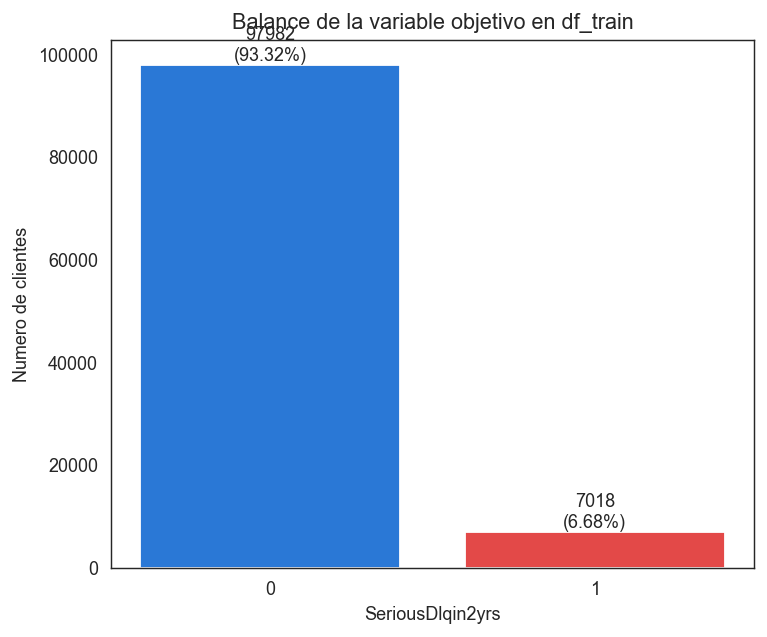
\includegraphics[width=.7\linewidth]{02_balance_target.png}
\caption{Distribuci\'on de la variable objetivo \texttt{SeriousDlqin2yrs} en el conjunto de entrenamiento.}
\label{fig:balance_target}
\end{figure}

El desbalance de clases es manejable: 93,3162\% de los clientes (97\,982 de 105\,000) pertenecen a la clase 0 (no impago) y 6,6838\% (7018) a la clase 1 (impago), es decir, aproximadamente 1 de cada 15 clientes impaga. Este ratio permite abordar el desbalance en la fase de modelado mediante ajuste de umbral o ponderaci\'on de clase, sin necesidad de t\'ecnicas de remuestreo agresivas en esta etapa exploratoria.

\subsection{Valores centinela y outliers}

Se identificaron valores centinela de codificaci\'on en las tres variables de morosidad (\texttt{NumberOfTime30-59DaysPastDueNotWorse}, \texttt{NumberOfTime60-89DaysPastDueNotWorse} y \texttt{NumberOfTimes90DaysLate}): los c\'odigos 96 y 98 aparecen de forma simult\'anea en las tres columnas para el mismo registro, un patr\'on incompatible con conteos reales de incidencias y t\'ipico de una codificaci\'on de ``dato no disponible'' o ``valor tope'' heredada del sistema origen. Junto a estos centinelas se cuantificaron outliers univariantes por rango l\'ogico y el resultado de un an\'alisis multivariante con Isolation Forest.

\begin{table}[H]
\centering
\caption{Resumen de valores centinela y outliers detectados en el conjunto de entrenamiento (105\,000 filas).}
\label{tab:centinelas_outliers}
\begin{tabular}{p{8.2cm}rr}
\toprule
Hallazgo & $n$ filas & \% filas \\
\midrule
\texttt{NumberOfTime*PastDue*} == 98 simult\'aneo en las 3 columnas & 185 & 0,1762 \\
\texttt{NumberOfTime*PastDue*} == 96 simult\'aneo en las 3 columnas & 3 & 0,0029 \\
\texttt{age} == 0 (edad inv\'alida) & 1 & 0,0010 \\
\texttt{RevolvingUtilizationOfUnsecuredLines} $>$ 2 (fuera de rango l\'ogico de un ratio) & 261 & 0,2486 \\
\texttt{DebtRatio} $>$ percentil 97,5 con \texttt{MonthlyIncome} nulo o $\leq$ 1 (posible artefacto de c\'alculo) & 2625 & 2,5000 \\
\bottomrule
\end{tabular}
\end{table}

En conjunto, los 188 registros con centinela 96/98 (0,1790\% del total) muestran una tasa de impago del 54,26\%, ocho veces superior al 6,60\% del resto de la poblaci\'on, lo que descarta que se trate de ruido aleatorio de captura. La \'ultima fila de la tabla anticipa el hallazgo central del preprocesado (secci\'on 4): 2625 filas (2,5000\% del total) combinan \texttt{DebtRatio} por encima del percentil 97,5 con \texttt{MonthlyIncome} no usable (nulo o $\leq$ 1), lo que apunta a un artefacto de c\'alculo -el numerador de deuda sin dividir- en lugar de variabilidad real del ratio.

\subsection{Multicolinealidad: correlaci\'on y factor de inflaci\'on de varianza}

Se calcularon las matrices de correlaci\'on de Pearson y de Spearman entre las diez variables explicativas, y el VIF de cada variable, definido para la variable $j$ como

\[
\mathrm{VIF}_j = \frac{1}{1 - R_j^2},
\]

donde $R_j^2$ es el coeficiente de determinaci\'on de la regresi\'on de la variable $j$ sobre el resto de variables explicativas. Valores de $\mathrm{VIF}_j > 10$ se consideran indicio de multicolinealidad severa.

\begin{figure}[H]
\centering
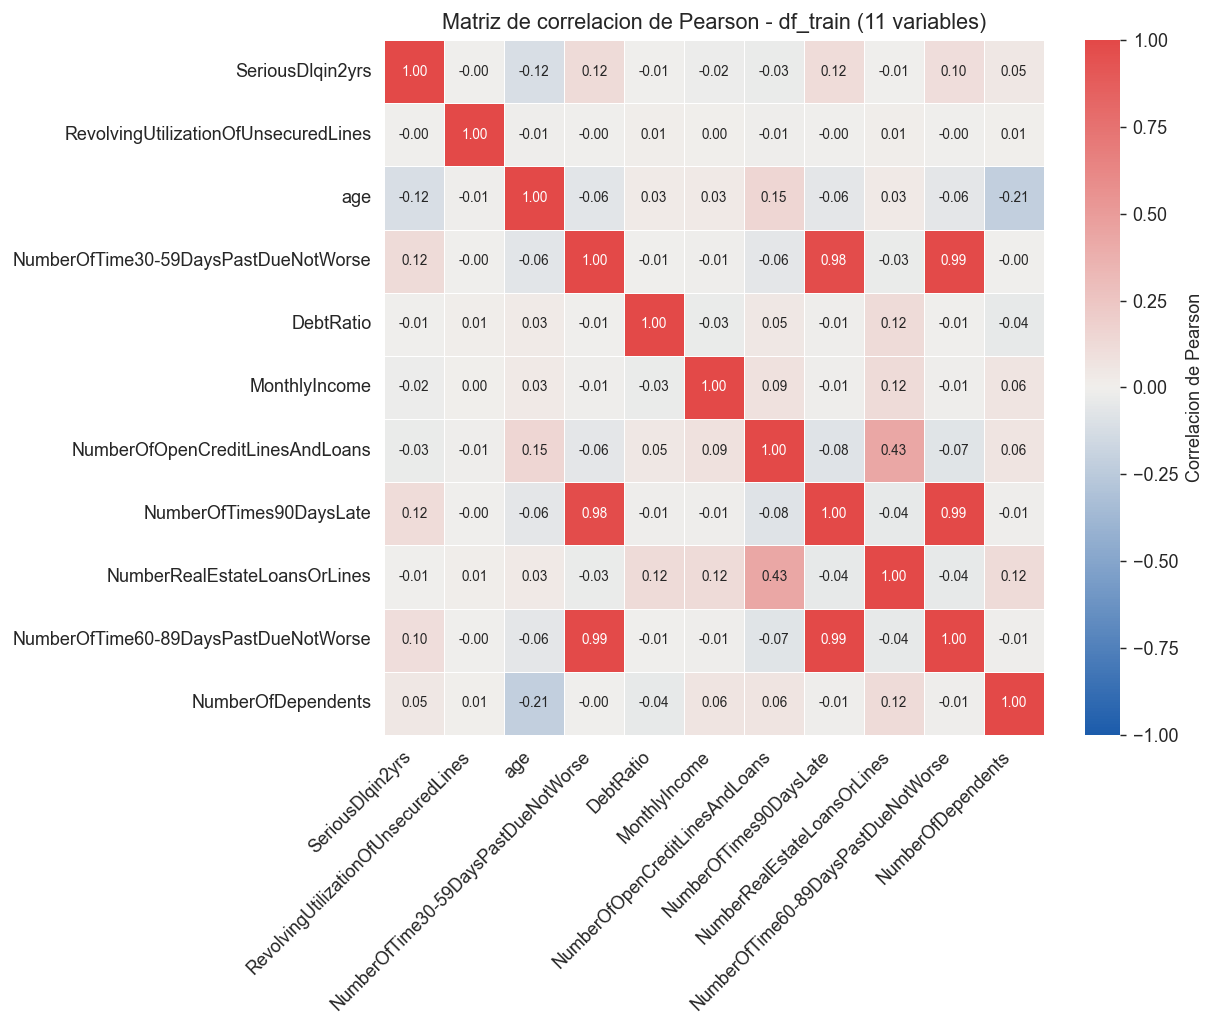
\includegraphics[width=.85\linewidth]{05_heatmap_correlacion_pearson.png}
\caption{Matriz de correlaci\'on de Pearson entre las variables explicativas del conjunto de entrenamiento.}
\label{fig:heatmap_pearson}
\end{figure}

\begin{figure}[H]
\centering
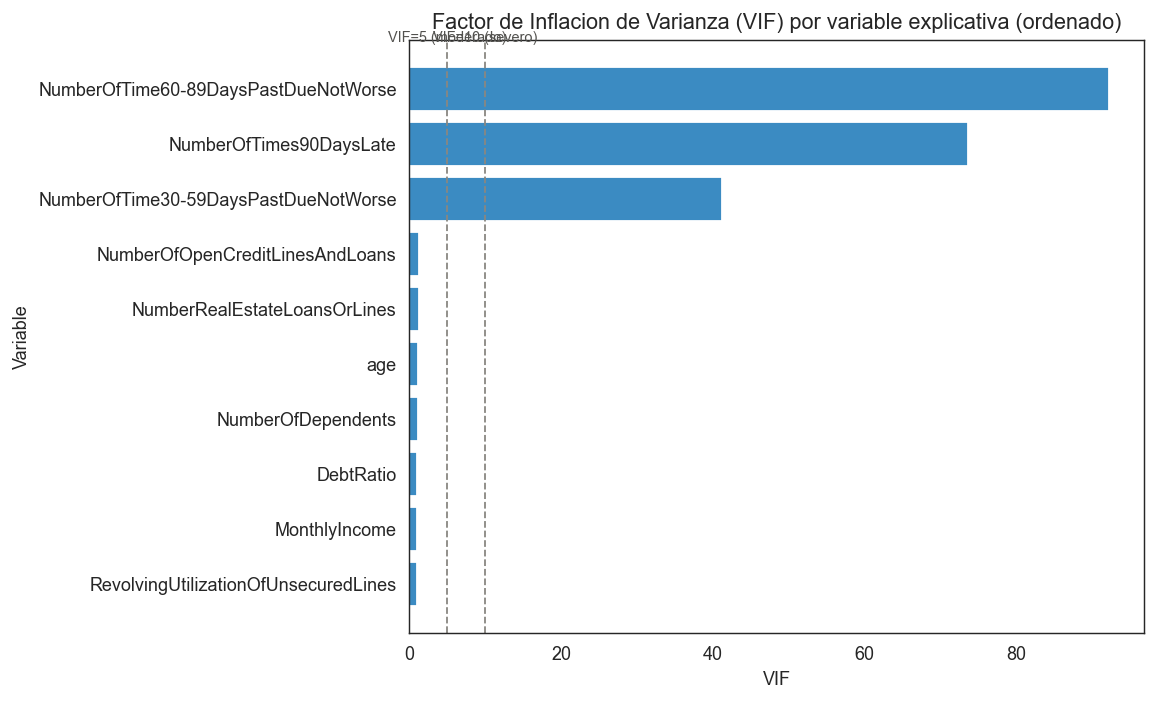
\includegraphics[width=.85\linewidth]{05_vif_barras.png}
\caption{Factor de Inflaci\'on de Varianza (VIF) por variable, conjunto de entrenamiento sin depurar.}
\label{fig:vif_barras}
\end{figure}

\begin{table}[H]
\centering
\caption{VIF por variable en el conjunto de entrenamiento (antes de tratar los centinelas).}
\label{tab:vif}
\begin{tabular}{lr}
\toprule
Variable & VIF \\
\midrule
\texttt{NumberOfTime60-89DaysPastDueNotWorse} & 92,30 \\
\texttt{NumberOfTimes90DaysLate} & 73,68 \\
\texttt{NumberOfTime30-59DaysPastDueNotWorse} & 41,29 \\
\texttt{NumberOfOpenCreditLinesAndLoans} & 1,29 \\
\texttt{NumberRealEstateLoansOrLines} & 1,27 \\
\texttt{age} & 1,09 \\
\texttt{NumberOfDependents} & 1,08 \\
\texttt{DebtRatio} & 1,02 \\
\texttt{MonthlyIncome} & 1,02 \\
\texttt{RevolvingUtilizationOfUnsecuredLines} & 1,00 \\
\bottomrule
\end{tabular}
\end{table}

El VIF severo ($>10$) se concentra exclusivamente en las tres variables de morosidad (92,30, 73,68 y 41,29), y su origen est\'a ligado a las 188 filas centinela descritas en la tabla \ref{tab:centinelas_outliers} (0,1790\% del dataset): al calcular la correlaci\'on de Spearman -menos sensible a valores extremos que Pearson- entre esas mismas tres variables, el coeficiente cae a un rango de 0,25-0,32, muy por debajo del 0,98-0,99 que arroja Pearson sobre los datos sin depurar. Esta discrepancia confirma que la multicolinealidad aparente es en gran medida un artefacto de un n\'umero reducido de observaciones con codificaci\'on centinela, no una relaci\'on lineal genuina y estable entre las tres variables.

\subsection{Mecanismo de ausencia en \texorpdfstring{\texttt{MonthlyIncome}}{MonthlyIncome} y \texorpdfstring{\texttt{NumberOfDependents}}{NumberOfDependents}}

Para diagnosticar el mecanismo de ausencia de las dos variables con nulos relevantes se cruz\'o su indicador de nulidad con el objetivo, con \texttt{DebtRatio} y con la edad.

\begin{figure}[H]
\centering
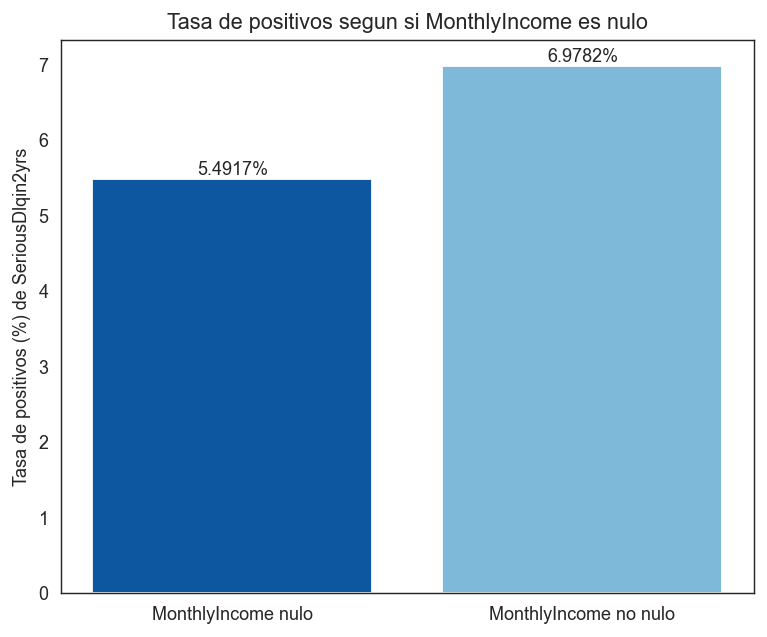
\includegraphics[width=.8\linewidth]{08_tasa_target_por_nulo_monthlyincome.png}
\caption{Tasa de impago seg\'un la nulidad de \texttt{MonthlyIncome}.}
\label{fig:tasa_target_nulo_income}
\end{figure}

\begin{figure}[H]
\centering
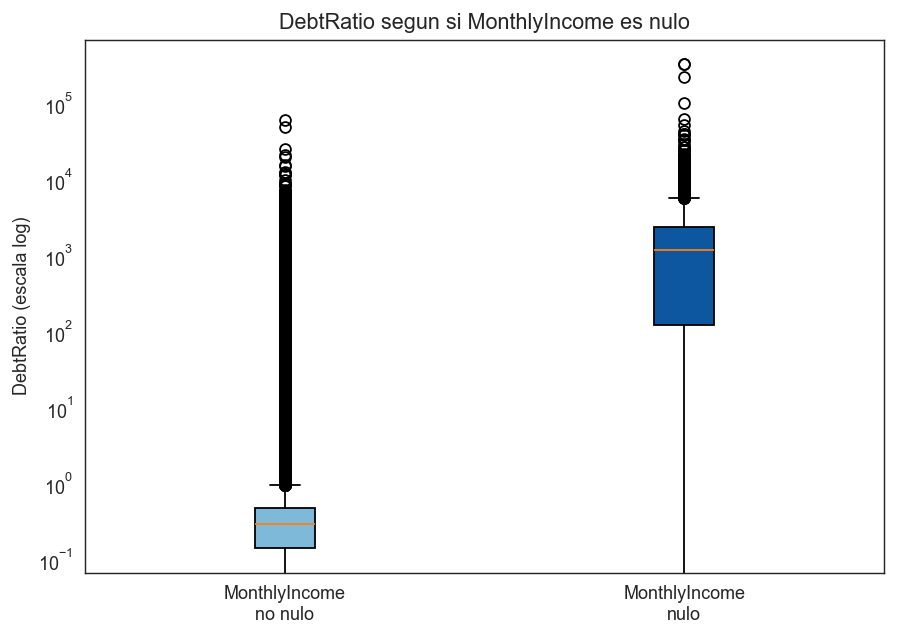
\includegraphics[width=.8\linewidth]{08_debtratio_boxplot_nulo_monthlyincome.png}
\caption{Distribuci\'on de \texttt{DebtRatio} seg\'un la nulidad de \texttt{MonthlyIncome}.}
\label{fig:debtratio_boxplot_nulo_income}
\end{figure}

El resultado es contraintuitivo: el grupo con \texttt{MonthlyIncome} nulo presenta una tasa de impago del 5,4917\%, frente al 6,9782\% del grupo con ingreso conocido -1,4865 puntos porcentuales menos-, pese a lo cual la diferencia es sistem\'atica y no aleatoria. Adem\'as, \texttt{DebtRatio} guarda en las filas de ingreso no usable el numerador crudo de deuda sin dividir: la mediana en ese subgrupo es 1181,0 frente a 0,2953 en el subgrupo con ingreso conocido (3999,32 veces mayor), y el 93,912\% de esas filas presenta \texttt{DebtRatio} $>$ 1, frente a solo el 6,0151\% en el resto -evidencia de un artefacto de c\'alculo, no de variabilidad real del ratio-. El nulo de \texttt{NumberOfDependents} (2738 filas, 2,6076\% del total) es adem\'as subconjunto exacto (100\%) del nulo de \texttt{MonthlyIncome}; ese subgrupo conjunto es sistem\'aticamente m\'as mayor (edad mediana 61 frente a 52 a\~nos) y con menor tasa de impago (4,6749\% frente a 6,7376\%). El conjunto de evidencias -sistematicidad, asociaci\'on con la edad y con el propio valor de \texttt{DebtRatio}- es compatible con un mecanismo de ausencia MNAR (\emph{missing not at random}): clientes de mayor edad con menos datos financieros registrados, no un fallo de captura independiente del valor no observado.

\subsection{An\'alisis de robustez}

Con el fin de comprobar si las filas centinela y los outliers extremos distorsionaban la estructura geom\'etrica de los datos, se recalcularon PCA, t-SNE y KernelPCA excluyendo dichas observaciones. La separaci\'on entre clases en las proyecciones resultantes no mejora al eliminarlas, lo que indica que el efecto de los centinelas se limita a las m\'etricas de correlaci\'on y VIF (secci\'on anterior) y no a la estructura real subyacente de los datos; en consecuencia, no se justifica eliminar estas filas del conjunto de entrenamiento, sino tratarlas expl\'icitamente como valores faltantes en el preprocesado (secci\'on 4).

\subsection*{Hallazgos}

\begin{itemize}
\item Desbalance manejable (aproximadamente 1 de cada 15 clientes en clase 1): 93,3162\% clase 0 (97\,982 filas) frente a 6,6838\% clase 1 (7018 filas).
\item Esquema y nulos casi id\'enticos entre entrenamiento y producci\'on, con una \'unica diferencia esperada (\texttt{dtype} del objetivo, vac\'io en producci\'on): \texttt{MonthlyIncome} 19,8048\% (entrenamiento) frente a 19,8578\% (producci\'on); \texttt{NumberOfDependents} 2,6076\% frente a 2,6356\% -parecidos, no id\'enticos-.
\item \texttt{DebtRatio} guarda el numerador crudo de deuda sin dividir cuando falta \texttt{MonthlyIncome}: mediana 1181,0 frente a 0,2953 con ingreso conocido (3999,32 veces mayor), y 93,912\% de esas filas presenta \texttt{DebtRatio} $>$ 1 frente a solo 6,0151\% en el resto: es un artefacto de c\'alculo, no variabilidad real.
\item Hallazgo contraintuitivo: el nulo de \texttt{MonthlyIncome} NO marca mayor riesgo -tasa de impago 5,4917\% (nulo) frente a 6,9782\% (conocido), 1,4865 puntos menos-, aunque la diferencia es sistem\'atica (no aleatoria): mejor preservarla con una variable indicadora que imputar y perder la se\~nal.
\item El nulo de \texttt{NumberOfDependents} (2738 filas, 2,6076\%) es subconjunto exacto (100\%) del nulo de \texttt{MonthlyIncome}; ese subgrupo es m\'as mayor (edad mediana 61 frente a 52 a\~nos) y con menor tasa de impago (4,6749\% frente a 6,7376\%): ambos nulos comparten un mismo mecanismo de ausencia MNAR, compatible con clientes mayores con menos datos financieros registrados.
\item VIF severo ($>10$) solo en las tres columnas de morosidad (92,30 / 73,68 / 41,29), inflado por 188 filas centinela (96 o 98 simult\'aneo en las tres columnas, 0,1790\% del dataset) con tasa de impago del 54,26\% -ocho veces el 6,60\% del resto-: la correlaci\'on de Spearman real cae a un rango de 0,25-0,32, muy por debajo del 0,98-0,99 de Pearson sobre los datos sin depurar.
\item El an\'alisis de robustez (PCA, t-SNE y KernelPCA recalculados sin los centinelas ni los outliers extremos) confirma que la separaci\'on entre clases no mejora al eliminarlos: el efecto de los centinelas recae sobre las m\'etricas de correlaci\'on y VIF, no sobre la estructura real de los datos.
\item Recomendaci\'on de imputaci\'on derivada del EDA: \texttt{MonthlyIncome} por mediana condicionada al tramo de edad (2800,0 en clientes de 30 a\~nos o menos frente a 6307,0 en el tramo 51-60, frente a 5400,0 de mediana global) m\'as variable indicadora de ausencia; \texttt{NumberOfDependents} por moda/mediana global (0) con su propia variable indicadora.
\end{itemize}

\section{Preprocesado}

Antes de aprender ning\'un par\'ametro se realiz\'o una partici\'on 80/20 estratificada (\texttt{random\_state=42}) del conjunto de entrenamiento \texttt{cs\_construccion.csv}: 84\,000 filas para entrenamiento y 21\,000 para test, con tasas de clase positiva casi id\'enticas entre s\'i (6.6833\% y 6.6857\%) y muy pr\'oximas a la tasa global del conjunto completo (6.6838\%, a solo 0.0024 puntos porcentuales de distancia). Todo lo que sigue -limpieza, imputaci\'on, rec\'alculo de variables, winsorizado y escalado- se ajusta \'unicamente sobre las 84\,000 filas de entrenamiento, nunca sobre test ni sobre producci\'on, para evitar fuga de informaci\'on.

\begin{table}[H]
\centering
\caption{Resumen de la partici\'on train/test sobre \texttt{cs\_construccion.csv}.}
\label{tab:split_resumen}
\begin{tabular}{lrrrr}
\toprule
Conjunto & $n$ filas & $n$ positivos & $n$ negativos & Tasa clase 1 \\
\midrule
Train & 84\,000 & 5\,614 & 78\,386 & 0.0668 \\
Test  & 21\,000 & 1\,404 & 19\,596 & 0.0669 \\
Total & 105\,000 & 7\,018 & 97\,982 & 0.0668 \\
\bottomrule
\end{tabular}
\end{table}

El orden real de las transformaciones sobre train es: (i) se limpia \texttt{age} (1 fila con \texttt{age==0}); (ii) se tratan como valores perdidos los c\'odigos centinela 96/98 simult\'aneos en las tres columnas de morosidad (149 filas, 0.1774\% del train); (iii) se imputa \texttt{MonthlyIncome} por la mediana del tramo de edad, excluyendo las filas de ingreso no usable; y (iv) se imputa \texttt{NumberOfDependents} por su moda (0). El desbalance de clases (6.68\%) no se corrige en esta fase: remuestrear antes de fijar el modelo introducir\'ia fuga de informaci\'on entre el ajuste de par\'ametros y la evaluaci\'on, de modo que se delega a la fase de modelado mediante \texttt{class\_weight} o ajuste del umbral de decisi\'on por coste.

\subsection{Hallazgo central: rec\'alculo del ratio de deuda (\texttt{DebtRatio})}

El hallazgo anal\'itico central del preprocesado es que el fichero de origen almacena, cuando el ingreso mensual no es utilizable, el \textbf{numerador crudo de deuda} en la columna \texttt{DebtRatio} en lugar del ratio propiamente dicho. Se define como ingreso no usable la uni\'on de dos subgrupos: ingreso nulo o ingreso $\leq 1$. Sobre train, \texttt{income\_no\_usable} comprende 17\,900 filas (21.3095\%): 16\,695 nulos m\'as 1\,205 con ingreso $\leq 1$. Un contraste $\chi^2$ entre ambos subgrupos frente al objetivo arroja $\chi^2 = 6.8716$, $p = 0.008758$: son estad\'isticamente distintos entre s\'i en tasa de riesgo. Aun as\'i, se fusionan en un \'unico indicador \texttt{is\_missing\_monthlyincome}, porque lo que comparten no es la tasa de riesgo sino el mismo mecanismo de corrupci\'on del numerador de deuda; es una decisi\'on de honestidad metodol\'ogica -reconocer que la fusi\'on no es estad\'isticamente perfecta- y no un atajo de conveniencia.

La correcci\'on aplicada a las filas de \texttt{income\_no\_usable} es

\[
\text{DebtRatio}_{\text{corregido}} \;=\; \frac{\text{DebtRatio}_{\text{crudo}}}{\text{MonthlyIncome}_{\text{imputado}}},
\]

es decir, se divide el numerador de deuda ya almacenado por el ingreso mensual una vez imputado (secci\'on \ref{sec:imputacion_income}), transformando un valor que hoy tiene unidades de moneda en un ratio adimensional comparable al del resto de la poblaci\'on.

\begin{figure}[H]
\centering
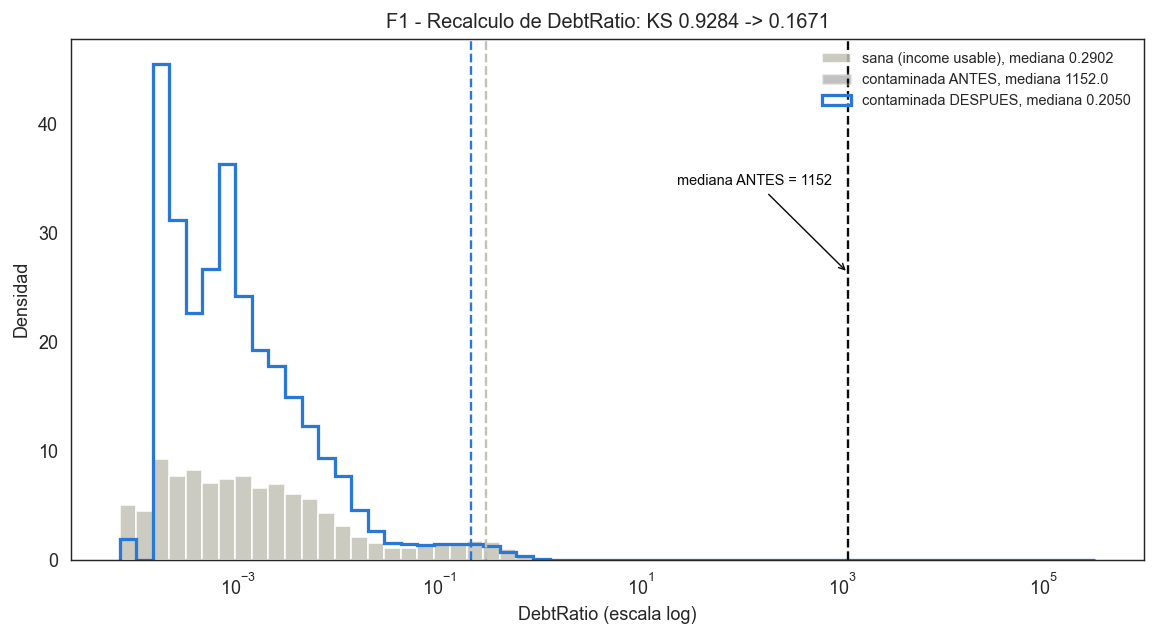
\includegraphics[width=.85\linewidth]{prep_01_debtratio_recalculo_validacion.png}
\caption{Distribuci\'on de \texttt{DebtRatio} en las filas de ingreso no usable antes (numerador crudo sin dividir) y despu\'es (dividido por el ingreso ya imputado) del rec\'alculo, frente al rango de la poblaci\'on con ingreso conocido.}
\label{fig:debtratio_recalculo}
\end{figure}

\begin{table}[H]
\centering
\caption{M\'etricas de validaci\'on del rec\'alculo de \texttt{DebtRatio}.}
\label{tab:debtratio_recalculo}
\begin{tabular}{lr}
\toprule
M\'etrica & Valor \\
\midrule
$n$ income\_no\_usable & 17\,900 \\
Mediana DebtRatio no usable (ANTES) & 1152.0000 \\
Mediana DebtRatio usable & 0.2902 \\
Ratio de medianas & 3969.4631 \\
Umbral percentil 97.5 de DebtRatio & 3538.0250 \\
$n$ cola $>$ percentil 97.5 & 2100 \\
\% cola que es income\_no\_usable & 100.0000 \\
Mediana DebtRatio no usable (DESPU\'ES) & 0.2050 \\
KS antes del rec\'alculo & 0.9284 \\
KS despu\'es del rec\'alculo & 0.1671 \\
$n$ filas recalculadas & 17\,900 \\
\bottomrule
\end{tabular}
\end{table}

El estad\'istico de Kolmogorov-Smirnov de dos muestras,
\[
D = \sup_x \left| F_{\text{contaminada}}(x) - F_{\text{sana}}(x) \right|,
\]
comparando la distribuci\'on de \texttt{DebtRatio} en las filas afectadas frente al resto de la poblaci\'on, cae de $D=0.9284$ antes del rec\'alculo a $D=0.1671$ despu\'es: las dos distribuciones pasan de ser casi disjuntas a solaparse de forma sustancial. Como consecuencia, el poder predictivo univariante de \texttt{DebtRatio} frente al objetivo -medido en AUC de un modelo de una sola variable- sube de 0.5212 (pr\'acticamente sin se\~nal) a 0.5531 tras la correcci\'on. La mediana de \texttt{DebtRatio} en las filas no usables pasa de 1152.0 (antes, frente a 0.2902 en las filas usables, un factor de $\sim$3970) a 0.2050 (despu\'es, ya comparable a la poblaci\'on general); adicionalmente, el 100\% de las 2\,100 filas situadas por encima del percentil 97.5 (umbral 3538.0250) antes del rec\'alculo correspond\'ia a \texttt{income\_no\_usable}, confirmando que esa cola era un artefacto de c\'alculo y no variabilidad real del ratio de deuda.

\subsection{Imputaci\'on de \texttt{MonthlyIncome} y \texttt{NumberOfDependents}}
\label{sec:imputacion_income}

\texttt{MonthlyIncome} se imputa por la mediana condicionada al tramo de edad del solicitante, no por la mediana global: la mediana global habr\'ia colapsado las 17\,900 filas con ingreso no usable a un \'unico valor (5460.0), generando un pico artificial en la distribuci\'on e ignorando el patr\'on real -en forma de U invertida- del ingreso mediano por tramo de edad.

\begin{figure}[H]
\centering
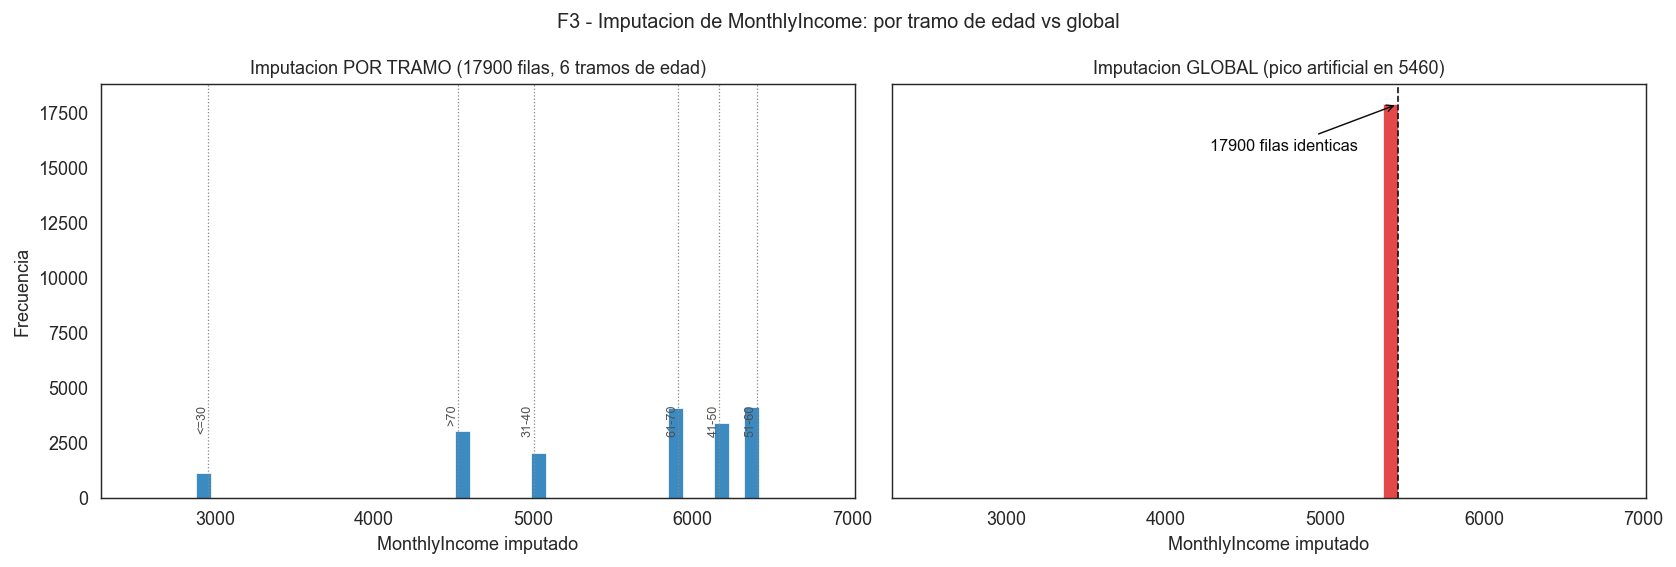
\includegraphics[width=.85\linewidth]{prep_03_imputacion_income_tramo_vs_global.png}
\caption{Mediana de \texttt{MonthlyIncome} por tramo de edad frente al valor \'unico que resultar\'ia de imputar por la mediana global.}
\label{fig:imputacion_income}
\end{figure}

\begin{table}[H]
\centering
\caption{Par\'ametros de imputaci\'on aprendidos sobre train.}
\label{tab:imputacion_parametros}
\begin{tabular}{lr}
\toprule
Par\'ametro & Valor \\
\midrule
Mediana de \texttt{age} & 52.0 \\
Mediana income, tramo $\leq$ 30 a\~nos & 2959.0 \\
Mediana income, tramo 31-40 a\~nos & 5000.0 \\
Mediana income, tramo 41-50 a\~nos & 6167.0 \\
Mediana income, tramo 51-60 a\~nos & 6400.0 \\
Mediana income, tramo 61-70 a\~nos & 5907.5 \\
Mediana income, tramo $>$ 70 a\~nos & 4526.0 \\
Mediana income global & 5460.0 \\
Moda de \texttt{NumberOfDependents} & 0.0 \\
\bottomrule
\end{tabular}
\end{table}

\texttt{NumberOfDependents} se imputa por su moda (0), coherente con el hallazgo de la fase de EDA de que su nulidad es subconjunto exacto del de \texttt{MonthlyIncome} y comparte el mismo mecanismo de ausencia. Todos los par\'ametros de imputaci\'on -medianas por tramo de edad, mediana global y moda- se aprenden exclusivamente sobre train y se congelan dentro del objeto \texttt{PreprocesadorCredito} para aplicarse sin reajuste a test y a producci\'on.

\subsection{Winsorizado, transformaci\'on logar\'itmica y escalado}

Tras la imputaci\'on y el rec\'alculo de \texttt{DebtRatio}, el pipeline aplica winsorizado seguido de transformaci\'on logar\'itmica y estandarizaci\'on. El winsorizado recorta cada variable a su percentil superior emp\'irico,
\[
x_{\text{winsor}} = \min\left(x,\; q_p\right),
\]
donde $q_p$ es el percentil $p$ estimado sobre train. \texttt{RevolvingUtilizationOfUnsecuredLines} se recorta al percentil 99 (cap $=1.102904$) y \texttt{DebtRatio} al percentil 99.9 (cap $=9.184215$), antes de aplicar la transformaci\'on logar\'itmica $x' = \log(1+x)$ (log1p) y, finalmente, el escalado est\'andar
\[
z = \frac{x - \mu_{\text{train}}}{\sigma_{\text{train}}},
\]
con $\mu_{\text{train}}$ y $\sigma_{\text{train}}$ estimados una \'unica vez sobre train y reutilizados sin reajuste en test y producci\'on.

El winsorizado no es redundante con el log1p: sobre \texttt{RevolvingUtilizationOfUnsecuredLines}, el sesgo (\emph{skewness}) crudo de 63.10 solo baja a 11.65 aplicando log1p sin recorte previo -insuficiente-, mientras que la combinaci\'on winsor+log1p lo reduce a 0.72. \texttt{age}, en cambio, queda deliberadamente excluida de la transformaci\'on logar\'itmica: su sesgo crudo (0.1909, ya pr\'oximo a la simetr\'ia) empeorar\'ia a $-0.4346$ si se le aplicara log1p. Los sesgos finales tras el pipeline completo son: Revolving 0.717, DebtRatio 2.3282, MonthlyIncome $-0.6159$ y age 0.1909.

\begin{figure}[H]
\centering
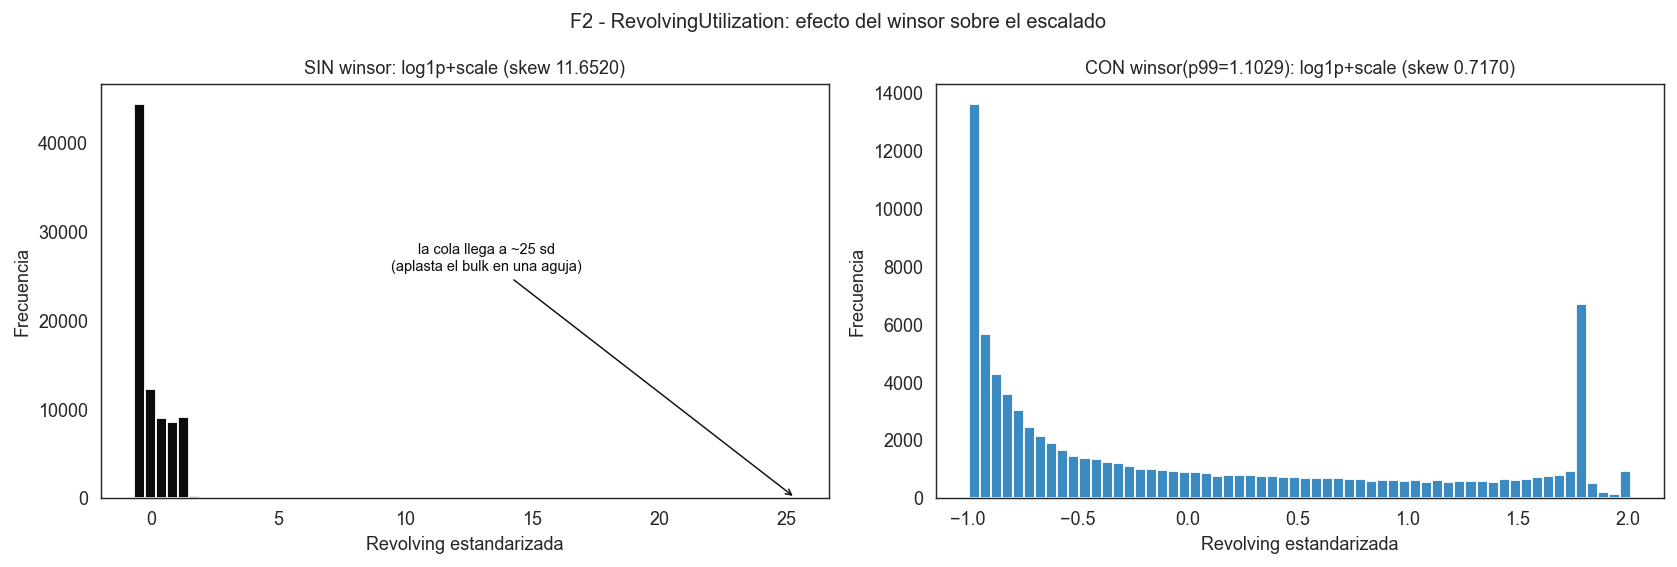
\includegraphics[width=.85\linewidth]{prep_02_revolving_winsor_efecto_escalado.png}
\caption{Distribuci\'on de \texttt{RevolvingUtilizationOfUnsecuredLines} antes del recorte (cola larga extrema) frente a despu\'es de winsorizado + log1p + escalado (forma casi sim\'etrica).}
\label{fig:winsor_revolving}
\end{figure}

\subsection{Multicolinealidad tras el tratamiento de los centinelas}

El VIF severo de las tres variables de morosidad, detectado en la fase de EDA sobre los datos sin depurar (40.90, 71.70 y 89.64), es en gran parte un artefacto de las 149 filas centinela (c\'odigos 96/98 simult\'aneos en las tres columnas), entre las que la correlaci\'on de Pearson m\'axima llega a 0.9926. Al tratar estos centinelas como valores perdidos en el preprocesado, el VIF de las tres variables colapsa a 1.18, 1.15 y 1.17, y la correlaci\'on de Pearson m\'axima entre ellas baja a 0.2995, recordando que
\[
\mathrm{VIF}_j = \frac{1}{1-R_j^2}.
\]
Las tres variables pueden por tanto incorporarse al modelo como \emph{features} independientes, sin necesidad de consolidarlas en un \'indice compuesto. El VIF m\'aximo de todas las variables del pipeline final es 1.9065, correspondiente a \texttt{DebtRatio}, sin indicios de multicolinealidad relevante.

\begin{table}[H]
\centering
\caption{VIF por variable, antes (datos sin depurar) y despu\'es del tratamiento de centinelas en el pipeline final.}
\label{tab:vif_antes_despues}
\begin{tabular}{lrr}
\toprule
Variable & VIF antes & VIF despu\'es \\
\midrule
\texttt{RevolvingUtilizationOfUnsecuredLines} & 1.0006 & 1.2498 \\
\texttt{age} & 1.0844 & 1.1709 \\
\texttt{NumberOfTime30-59DaysPastDueNotWorse} & 40.8977 & 1.1781 \\
\texttt{DebtRatio} & 1.0240 & 1.9065 \\
\texttt{MonthlyIncome} & 1.0160 & 1.5578 \\
\texttt{NumberOfOpenCreditLinesAndLoans} & 1.2860 & 1.4221 \\
\texttt{NumberOfTimes90DaysLate} & 71.6977 & 1.1494 \\
\texttt{NumberRealEstateLoansOrLines} & 1.2755 & 1.8750 \\
\texttt{NumberOfTime60-89DaysPastDueNotWorse} & 89.6394 & 1.1720 \\
\texttt{NumberOfDependents} & 1.0787 & 1.1171 \\
\bottomrule
\end{tabular}
\end{table}

\subsection{Contrato de salida y verificaci\'on de fuga de informaci\'on}

El pipeline entrega tres tablas: train (84\,000 $\times$ 13), test (21\,000 $\times$ 13) y producci\'on (45\,000 $\times$ 14, con la columna adicional \texttt{id\_fila\_original} para trazabilidad). Cada tabla contiene 10 variables continuas en \texttt{float64} m\'as 2 indicadores en \texttt{int8} (\texttt{is\_missing\_monthlyincome} y \texttt{es\_centinela\_pastdue}). Una bater\'ia de 9 aserciones autom\'aticas (A-I) certifica el contrato antes de dar el pipeline por v\'alido:

\begin{itemize}
\item Reproducibilidad exacta del objeto serializado (tolerancia $\text{atol}=0$).
\item Esquema de columnas y ausencia total de valores \texttt{NaN}.
\item Conteo de filas correcto en cada partici\'on.
\item Apatridia por lote: procesar una fila aislada o el lote completo produce el mismo resultado fila a fila (tolerancia $\text{atol}=10^{-12}$).
\item El ajuste (\texttt{fit}) us\'o exclusivamente train, nunca test ni producci\'on.
\item Invarianza al orden de las filas de entrada (permutar el orden no altera el resultado).
\item Robustez ante valores de producci\'on no vistos en train -por ejemplo, un valor de \texttt{RevolvingUtilizationOfUnsecuredLines} $=50708$ se recorta correctamente al cap de entrenamiento, 1.102904-.
\item Idempotencia al releer el objeto \texttt{PreprocesadorCredito} guardado en disco.
\end{itemize}

\begin{figure}[H]
\centering
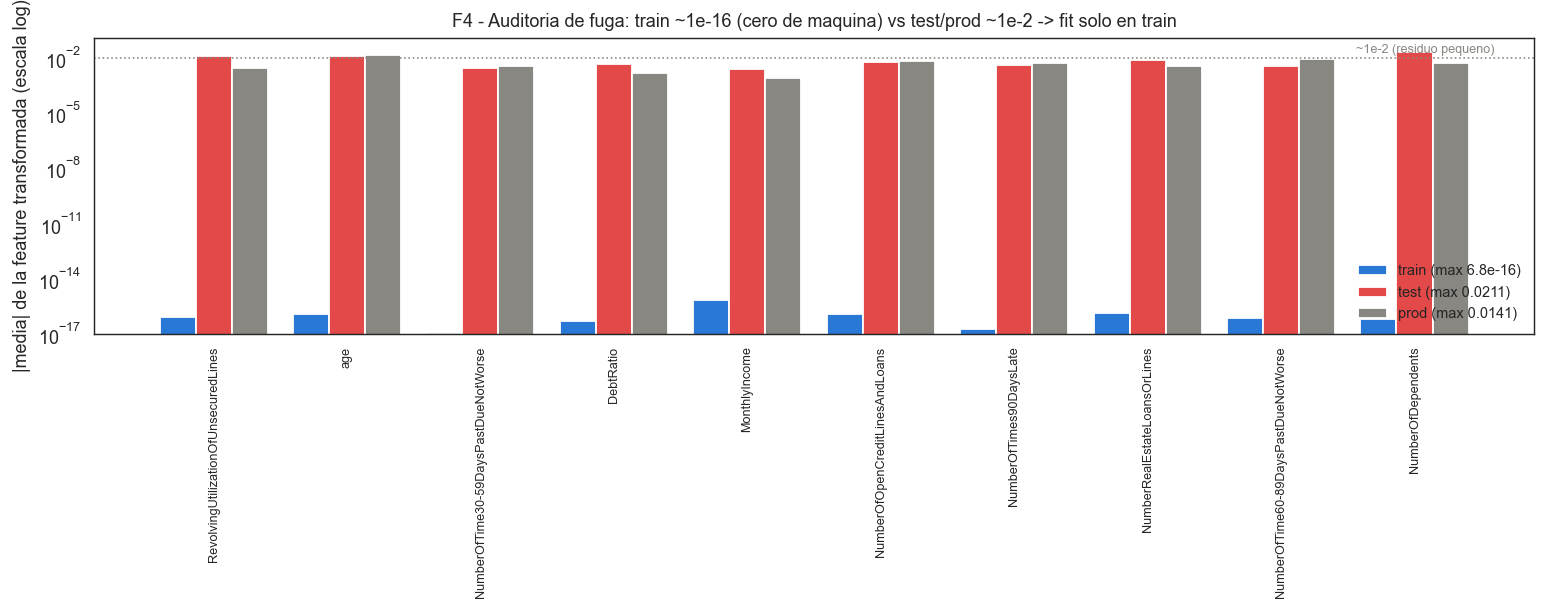
\includegraphics[width=.85\linewidth]{prep_04_auditoria_fuga_medias.png}
\caption{Media absoluta de las variables preprocesadas por conjunto: train, test y producci\'on.}
\label{fig:auditoria_fuga}
\end{figure}

La comprobaci\'on m\'as directa de ausencia de fuga es la media absoluta de las variables ya escaladas en cada conjunto: en train se sit\'ua en $\sim 6.83 \times 10^{-16}$ -esencialmente cero de m\'aquina, como corresponde a un escalado est\'andar ajustado sobre los mismos datos-, frente a 0.021086 en test y 0.014083 en producci\'on. El salto de aproximadamente 14 \'ordenes de magnitud entre train y los otros dos conjuntos es la evidencia emp\'irica de que el ajuste del escalador no vio ni test ni producci\'on durante el \texttt{fit}.

\subsection*{Hallazgos}

\begin{itemize}
\item El split preserva el desbalance real de clases: 84\,000 filas de train frente a 21\,000 de test, con tasas de clase positiva de 6.6833\% y 6.6857\% (0.0024 puntos porcentuales de diferencia); el indicador \texttt{es\_centinela\_pastdue} dispara la tasa del objetivo hasta 53.69\%, frente a 6.60\% en el resto de la poblaci\'on ($\sim$8 veces), evidencia de que no es ruido de captura.
\item El rec\'alculo de \texttt{DebtRatio} confirma la hip\'otesis planteada en el EDA: el estad\'istico KS pasa de 0.9284 a 0.1671, el AUC univariante de 0.5212 a 0.5531, y la mediana de las filas no usables de 1152.0 a 0.2050 tras dividir por el ingreso ya imputado.
\item El VIF de las tres variables de morosidad cae de 40.90/71.70/89.64 a $\sim$1.2 al tratar como perdidas las 149 filas centinela; el VIF m\'aximo de todo el conjunto final de variables es 1.9065 (\texttt{DebtRatio}), sin indicios de multicolinealidad relevante.
\item La auditor\'ia de fuga muestra una media absoluta de las variables de $\sim 6.83 \times 10^{-16}$ en train frente a 0.021086 en test y 0.014083 en producci\'on -un salto de $\sim$14 \'ordenes de magnitud-, reforzada por 9 aserciones (A-I) que incluyen apatridia por lote e invarianza a la permutaci\'on del orden de las filas.
\item Nota de calidad de datos: 107 filas de test (0.51\%) tienen una fila ``gemela'' exacta en train (id\'enticas en las 10 variables originales y en el objetivo); el impacto pr\'actico en el escenario de coste sim\'etrico es pr\'acticamente nulo, pero se deja constancia expl\'icita de la existencia de duplicados repartidos entre particiones.
\item Decisi\'on expl\'icita de dise\~no: el desbalance de clases (6.68\%) no se corrige en el preprocesado, porque remuestrear antes de fijar el modelo constituir\'ia fuga de informaci\'on; se delega a la fase de modelado mediante \texttt{class\_weight} o ajuste del umbral de decisi\'on por coste (secciones 5 y 6).
\end{itemize}

\section{Modelo: escenario de coste sim\'etrico ($C_{FP} = C_{FN} = 1$)}
\label{sec:modelo-simetrico}

\subsection{Planteamiento y convenci\'on de costes}

La convenci\'on de coste queda fijada sin ambig\"uedad antes de entrenar ning\'un modelo. Se define
como clase positiva el impago (\texttt{SeriousDlqin2yrs=1}); una predicci\'on $\hat y = 1$ significa
\emph{denegar} el cr\'edito y $\hat y = 0$ significa \emph{conceder}lo. En este marco, un falso
negativo (FN) equivale a conceder cr\'edito a un solicitante que despu\'es impaga --el error caro
desde el punto de vista del negocio--, mientras que un falso positivo (FP) equivale a denegar
cr\'edito a un buen pagador. Los aciertos (TP y TN) no generan coste. En este primer escenario ambos
tipos de error se penalizan por igual: $C_{FP} = C_{FN} = 1$.

Se comparan cinco familias de modelos con interfaz com\'un \texttt{predict}/\texttt{predict\_proba}:
regresi\'on log\'istica, XGBoost, una red neuronal peque\~na (MLP), una red neuronal profunda (MLP) y
un bandit contextual LinUCB. Ninguna de ellas reponde las clases (sin \emph{SMOTE} ni
\texttt{class\_weight}): bajo una matriz de coste asim\'etrica la respuesta metodol\'ogicamente
correcta es desplazar el \textbf{umbral} de decisi\'on aplicado a la probabilidad estimada, no
distorsionar la probabilidad misma alterando el proceso de entrenamiento.

\subsection{Metodolog\'ia: validaci\'on cruzada, probabilidades OOF y umbral \'optimo}

La comparaci\'on de familias y la b\'usqueda del umbral se realizan con validaci\'on cruzada
estratificada de 5 particiones (folds) sobre el conjunto de entrenamiento, utilizando siempre las
probabilidades \emph{out-of-fold} (OOF) concatenadas de las 84\,000 observaciones de train --nunca
las de test--, precisamente para evitar fuga de informaci\'on: optimizar el umbral directamente sobre
test contaminar\'ia la misma cifra que despu\'es se reporta como resultado final.

El coste esperado emp\'irico para un umbral $\theta$ se define como el coste medio por solicitante:

\[
\text{Coste}(\theta) \;=\; \frac{1}{n}\sum_{i=1}^{n}
\Big[\, C_{FP}\cdot \mathbf{1}\big(y_i=0,\ \hat y_i(\theta)=1\big)
\;+\; C_{FN}\cdot \mathbf{1}\big(y_i=1,\ \hat y_i(\theta)=0\big) \,\Big]
\]

donde $\hat y_i(\theta) = \mathbf{1}(p_i \geq \theta)$ y $p_i$ es la probabilidad de impago estimada
para el solicitante $i$. El umbral operativo se obtiene por b\'usqueda exhaustiva (\emph{argmin}) del
coste sobre las probabilidades OOF:

\[
\theta_{\text{OOF}}^{*} \;=\; \arg\min_{\theta \in [0,1]} \text{Coste}(\theta)
\]

y se contrasta con el umbral \'optimo anal\'itico, que se deriva minimizando el coste esperado bajo la
probabilidad estimada e iguala el coste marginal de ambos tipos de error:

\[
\theta^{*} \;=\; \frac{C_{FP}}{C_{FP}+C_{FN}}
\]

que para el escenario sim\'etrico da $\theta^{*} = 1/2 = 0.5$. Al no producir una probabilidad
calibrada ni un umbral expl\'icito, LinUCB se eval\'ua por su acci\'on \emph{greedy} OOF (denegar si la
recompensa esperada de conceder es negativa). El modelo ganador se reentrena sobre el 100\% de
train con su umbral de validaci\'on cruzada y se eval\'ua una \'unica vez sobre el conjunto de test,
frente a dos referencias triviales: conceder cr\'edito a todos los solicitantes y denegarlo a todos.

\subsection{Comparaci\'on de familias por validaci\'on cruzada}

\begin{table}[H]
\centering
\caption{Comparaci\'on de familias de modelos por coste esperado en CV(5) sobre probabilidades OOF.}
\label{tab:comparacion-familias-c1}
\begin{tabular}{llrrrr}
\toprule
Familia & Modelo & Coste CV & Umbral & AUC & Tasa denegaci\'on CV \\
\midrule
Boosted        & XGBoost        & 0.0623 & 0.4934 & 0.8642 & 0.0233 \\
Neuronal       & MLP peque\~na  & 0.0624 & 0.4891 & 0.8617 & 0.0201 \\
Neuronal       & MLP profunda   & 0.0626 & 0.4759 & 0.8630 & 0.0185 \\
Lineal         & Log\'istica    & 0.0629 & 0.4837 & 0.8515 & 0.0205 \\
Bandit         & LinUCB         & 0.0629 & N/D    & N/D    & 0.0214 \\
Baseline       & Conceder-todo  & 0.0668 & N/D    & N/D    & 0.0000 \\
Baseline       & Denegar-todo   & 0.9332 & N/D    & N/D    & 1.0000 \\
\bottomrule
\end{tabular}
\end{table}

\begin{figure}[H]
\centering
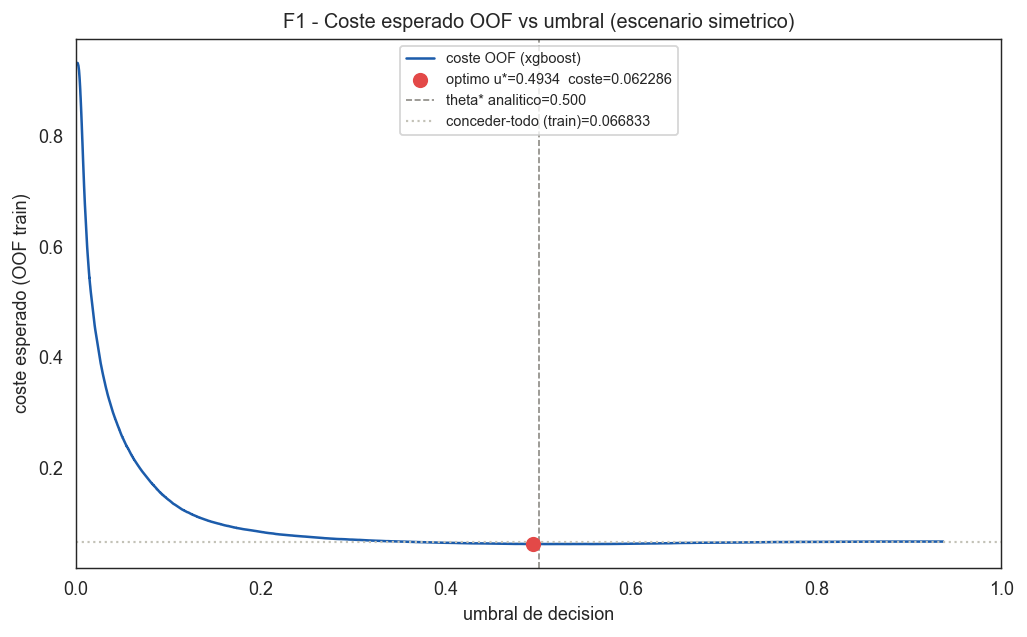
\includegraphics[width=.85\linewidth]{mod_03_coste_vs_umbral.png}
\caption{Coste esperado OOF en funci\'on del umbral de decisi\'on. La curva es notablemente plana en
el entorno del \'optimo emp\'irico ($\theta_{\text{OOF}}^{*}=0.4934$), que cae muy cerca de la
vertical anal\'itica $\theta^{*}=0.5$.}
\label{fig:coste-vs-umbral-c1}
\end{figure}

\begin{figure}[H]
\centering
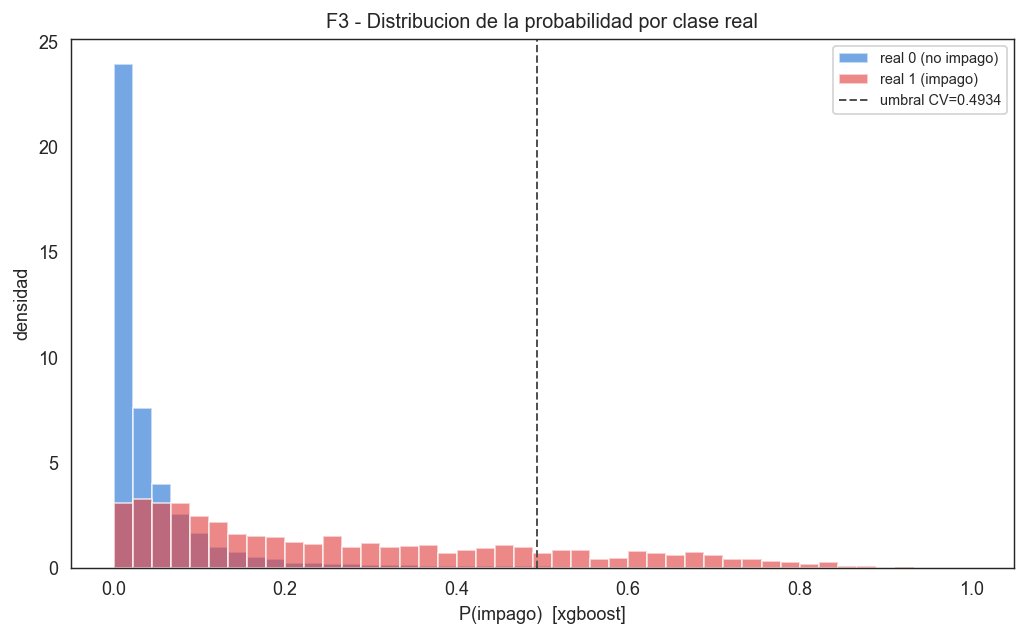
\includegraphics[width=.85\linewidth]{mod_03_distribucion_proba.png}
\caption{Distribuci\'on de la probabilidad de impago estimada, $P(\text{impago})$, seg\'un la clase
real en test. El solapamiento sustancial entre ambas clases alrededor del umbral explica por qu\'e el
coste global resulta bajo aunque el \emph{recall} tambi\'en lo sea.}
\label{fig:distribucion-proba-c1}
\end{figure}

\begin{figure}[H]
\centering
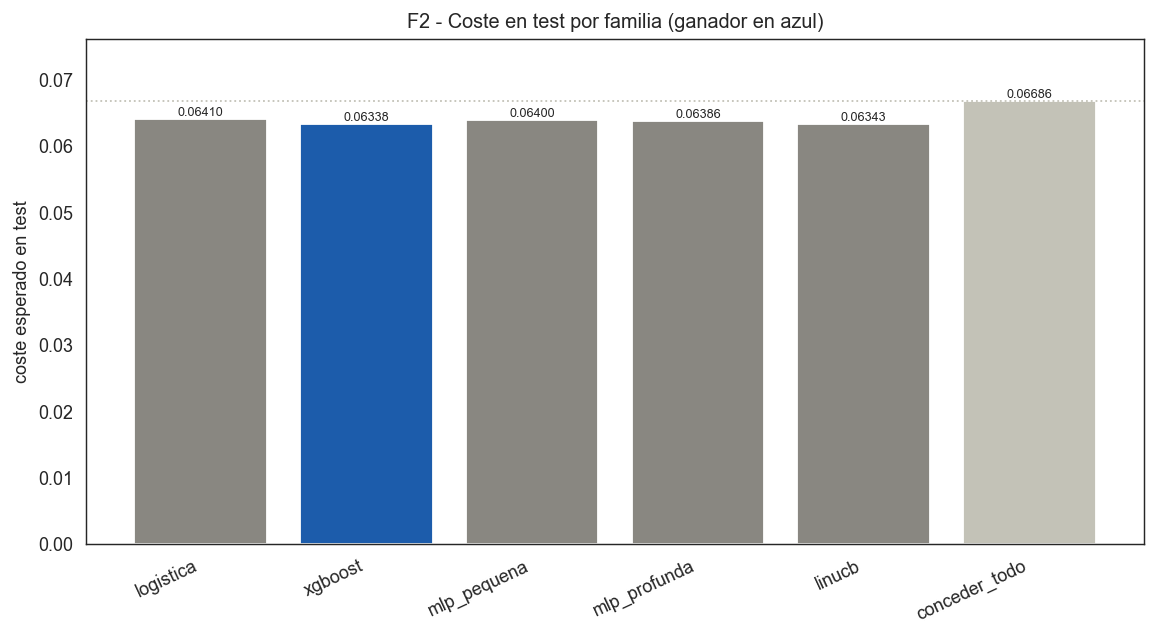
\includegraphics[width=.85\linewidth]{mod_03_comparacion_familias.png}
\caption{Coste en test por familia de modelo (el ganador, XGBoost, destacado), frente a la l\'inea
punteada del baseline de conceder-todo.}
\label{fig:comparacion-familias-c1}
\end{figure}

\subsubsection*{Hallazgos de la selecci\'on de modelo (CV(5), OOF)}

\begin{itemize}
\item Gana XGBoost con $\text{coste}_{\text{CV}}=0.062286$, seguido de cerca por MLP peque\~na
($0.062440$), MLP profunda ($0.062619$), log\'istica ($0.062917$) y LinUCB ($0.062929$). La familia de
modelo casi no importa en este escenario: el margen entre log\'istica y XGBoost es de solo
$0.000631$, dentro del ruido de estimaci\'on.
\item El umbral \'optimo emp\'irico OOF, $\theta_{\text{OOF}}^{*}=0.493394$, es pr\'acticamente
id\'entico al \'optimo anal\'itico $\theta^{*}=0.5$, lo que confirma la teor\'ia y revela una curva de
coste casi degenerada: este es un escenario poco exigente para discriminar entre familias (el
escenario informativo es el asim\'etrico, tratado en la secci\'on siguiente).
\item A igual capacidad \emph{lineal}, LinUCB (bandit) pr\'acticamente empata con la regresi\'on
log\'istica ($0.062929$ frente a $0.062917$): el bandit no resulta inferior al aprendizaje supervisado
cuando ambos compiten con la misma capacidad de modelo. La ventaja de XGBoost procede de su
\emph{capacidad} (boosting de \'arboles), no del mero hecho de ser supervisado. Se elige el modelo
supervisado por auditabilidad y calibraci\'on --probabilidad interpretable, sin el \emph{regret} de
exploraci\'on propio de un bandit-- y no por una superioridad intr\'inseca del paradigma.
\end{itemize}

\subsection{Umbral \'optimo, evaluaci\'on en test y matriz de confusi\'on}

\begin{table}[H]
\centering
\caption{S\'intesis del modelo ganador (XGBoost) en el escenario de coste sim\'etrico.}
\label{tab:umbral-c1}
\begin{tabular}{lr}
\toprule
M\'etrica & Valor \\
\midrule
Umbral \'optimo (OOF)                  & 0.4934 \\
Umbral anal\'itico ($\theta^{*}$)      & 0.5000 \\
Coste CV                               & 0.0623 \\
Coste test                             & 0.0634 \\
Coste conceder-todo                    & 0.0669 \\
Coste denegar-todo                     & 0.9331 \\
Mejora relativa vs.\ conceder-todo     & 5.20\% \\
\bottomrule
\end{tabular}
\end{table}

\begin{table}[H]
\centering
\caption{Matriz de confusi\'on en test con el umbral \'optimo $\theta_{\text{OOF}}^{*}=0.4934$.}
\label{tab:confusion-c1}
\begin{tabular}{lrr}
\toprule
 & Predicho: conceder & Predicho: denegar \\
\midrule
Real: buen pagador & 19\,383 & 213 \\
Real: moroso       & 1\,118  & 286 \\
\bottomrule
\end{tabular}
\end{table}

\begin{figure}[H]
\centering
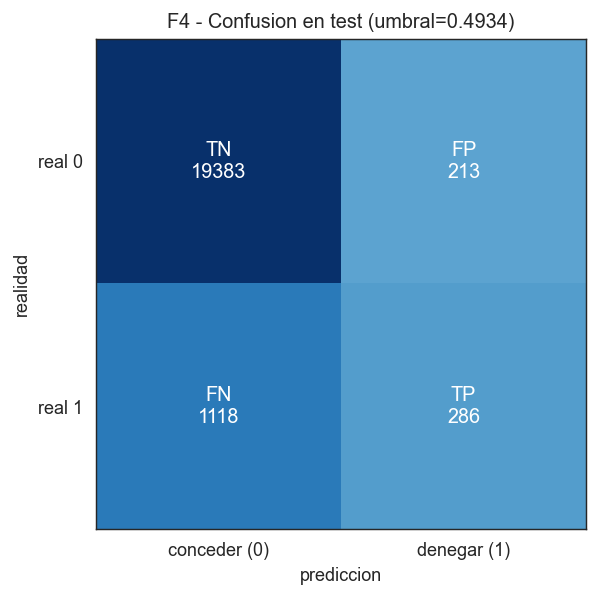
\includegraphics[width=.7\linewidth]{mod_03_confusion_optimo.png}
\caption{Matriz de confusi\'on en test (mapa de calor) con el umbral \'optimo del escenario
sim\'etrico. Los falsos negativos (1\,118) superan con creces a los falsos positivos (213), coherente
con la precisi\'on y el \emph{recall} obtenidos.}
\label{fig:confusion-c1}
\end{figure}

\subsubsection*{Hallazgos de test y producci\'on}

\begin{itemize}
\item En test, el coste alcanzado por el modelo ganador es $0.063381$, frente a $0.066857$ del
baseline de conceder-todo (mejora relativa de $5.1994\%$) y muy por debajo de $0.933143$ del
baseline de denegar-todo.
\item M\'etricas de contexto del ganador en test --no determinan el umbral, se reportan como
referencia--: precisi\'on $=0.573146$, \emph{recall} $=0.203704$, AUC $=0.870109$. Matriz de
confusi\'on cruda: $TN=19\,383$, $FP=213$, $FN=1\,118$, $TP=286$.
\item Un \emph{bootstrap} pareado ($B=5000$, semilla 42) del margen (\emph{edge}) del ganador frente a
conceder-todo da un edge medio de $0.003476$ ($5.20\%$ del coste del baseline), con intervalo de
confianza al 95\% de $[0.001381,\ 0.005571]$ y $P(\text{edge}\leq 0)=0.0008$: la mejora es peque\~na
en t\'erminos absolutos pero estad\'isticamente significativa.
\item La transferencia de test a producci\'on se verifica con un tama\~no de efecto de
Kolmogorov--Smirnov $D=0.011800$ (despreciable) entre las distribuciones de $P(\text{impago})$ en
ambos conjuntos, medias muy pr\'oximas ($0.068223$ en test frente a $0.067049$ en producci\'on) y
tasas de denegaci\'on casi id\'enticas ($0.023762$ frente a $0.023556$, diferencia $0.000206$): el
\emph{scoring} generaliza sin desplazamiento material, bajo el supuesto --no verificable sin
etiquetas-- de que la prevalencia real en producci\'on se mantiene estable.
\item El entregable oficial \texttt{cs\_produccion1.csv} (45\,000 filas) se verifica con 5
comprobaciones bloqueantes (\emph{asserts}): objetivo en $\{0,1\}$ sin valores nulos, columnas y orden
originales preservados, y cobertura exacta de \'indices $0$ a $44\,999$. La tasa de denegaci\'on en
producci\'on es del $2.3556\%$ ($1\,060$ de $45\,000$ solicitantes), coherente con un escenario de
coste sim\'etrico que deniega poco.
\end{itemize}

\section{Modelo -- escenario de coste asim\'etrico ($C_{FN} = 10\cdot C_{FP}$)}

\subsection{Planteamiento y reutilizaci\'on del modelo}

En este escenario un falso negativo (conceder cr\'edito a un solicitante que posteriormente
impaga) se penaliza diez veces m\'as que un falso positivo (denegar cr\'edito a un buen
pagador): $C_{FP}=1$, $C_{FN}=10$. No se reentrena ning\'un modelo nuevo: se reutiliza el
mismo XGBoost ganador del escenario sim\'etrico (secci\'on anterior) junto con las mismas
84\,000 probabilidades \emph{out-of-fold} (OOF) de entrenamiento, con coincidencia byte a
byte verificada frente al escenario sim\'etrico. Bajo una matriz de coste asim\'etrica no es
necesario alterar el modelo probabil\'istico subyacente: basta con desplazar el
\textbf{umbral de decisi\'on} que convierte la probabilidad estimada de impago,
$\hat p_i = \hat P(y_i=1\mid x_i)$, en una decisi\'on binaria de conceder/denegar. De este
modo, un \'unico modelo con dos umbrales distintos cubre ambos escenarios de negocio.

La regla de decisi\'on parametrizada por el umbral $\theta$ es
\[
\hat y_i(\theta) = \mathbf{1}\left(\hat p_i \geq \theta\right), \qquad
\hat y_i = 1 \;\Rightarrow\; \text{denegar}, \qquad \hat y_i = 0 \;\Rightarrow\; \text{conceder},
\]
y el coste esperado emp\'irico asociado a un umbral $\theta$, evaluado sobre un conjunto de
$N$ observaciones con etiqueta real $y_i$, es
\[
\mathrm{Coste}(\theta) = \frac{1}{N}\sum_{i=1}^{N}
\Big[ C_{FP}\cdot \mathbf{1}\big(y_i=0,\ \hat y_i(\theta)=1\big)
+ C_{FN}\cdot \mathbf{1}\big(y_i=1,\ \hat y_i(\theta)=0\big) \Big].
\]
El umbral \'optimo emp\'irico se obtiene por b\'usqueda exhaustiva (argm\'in) de esta funci\'on
sobre las probabilidades OOF de entrenamiento, evitando por construcci\'on cualquier fuga de
informaci\'on desde el conjunto de test. Ese umbral emp\'irico se contrasta con el \'optimo
anal\'itico derivado de igualar el coste marginal esperado de ambas clases de error,
\[
\theta^{*} = \frac{C_{FP}}{C_{FP}+C_{FN}}.
\]
Con $C_{FP}=1$ y $C_{FN}=10$, el umbral anal\'itico te\'orico es $\theta^{*} = 1/11 = 0.0909$.

\subsection{Umbral \'optimo y coste esperado}

El umbral \'optimo emp\'irico cae de $0.4934$ (escenario sim\'etrico) a $\mathbf{0.0906}$ en
el escenario asim\'etrico, pr\'acticamente coincidente con el $0.0909$ anal\'itico. La
Figura~\ref{fig:mod04-comparacion-escenarios} contrasta ambos escenarios y la
Figura~\ref{fig:mod04-coste-vs-umbral} muestra la curva de coste OOF frente al umbral con el
\'optimo emp\'irico marcado.

\begin{figure}[H]
\centering
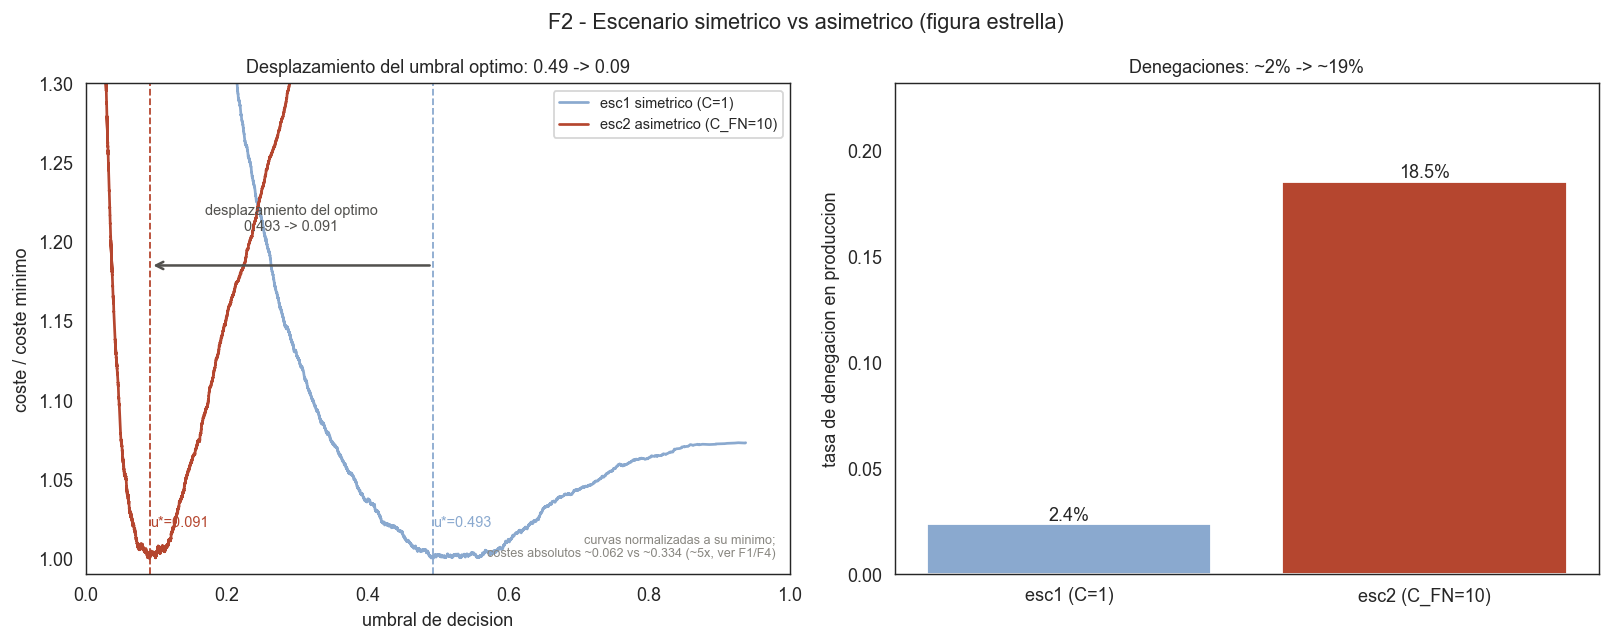
\includegraphics[width=.85\linewidth]{mod_04_comparacion_escenarios.png}
\caption{Comparaci\'on del escenario sim\'etrico y el escenario asim\'etrico sobre el mismo
modelo XGBoost: cambia \'unicamente el umbral de decisi\'on aplicado a la misma probabilidad
estimada.}
\label{fig:mod04-comparacion-escenarios}
\end{figure}

\begin{figure}[H]
\centering
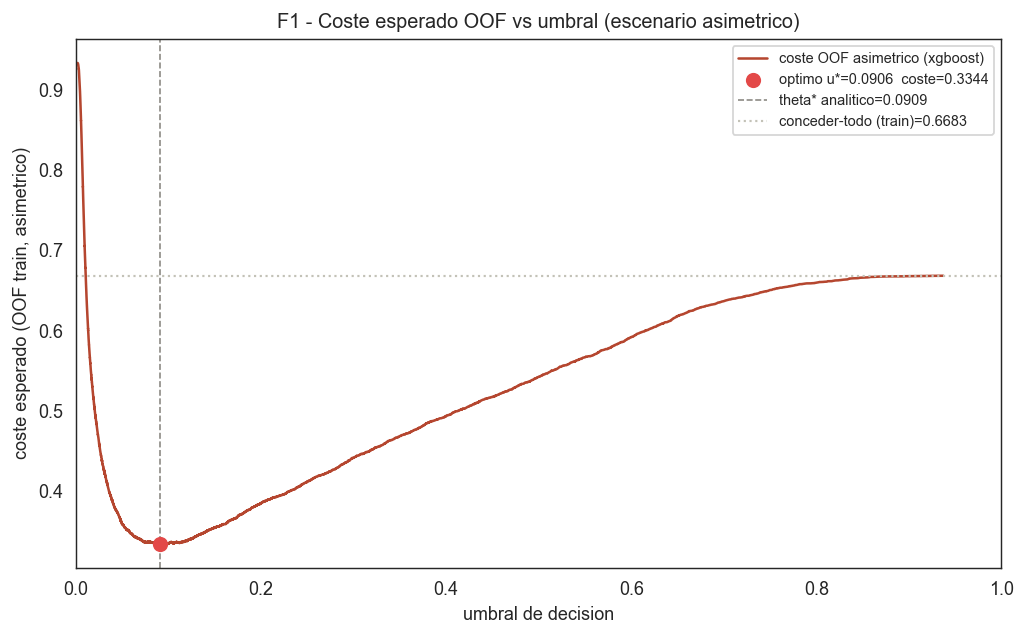
\includegraphics[width=.85\linewidth]{mod_04_coste_vs_umbral.png}
\caption{Coste esperado OOF en funci\'on del umbral de decisi\'on, escenario $C_{FN}=10\cdot
C_{FP}$. El m\'inimo emp\'irico (umbral $0.0906$) queda pr\'acticamente sobre la vertical
anal\'itica te\'orica ($1/11=0.0909$).}
\label{fig:mod04-coste-vs-umbral}
\end{figure}

\begin{table}[H]
\centering
\caption{Resultados del escenario asim\'etrico (\texttt{coste10}) para el modelo XGBoost
ganador, umbral fijado por validaci\'on cruzada sobre probabilidades OOF y evaluado una
\'unica vez en test.}
\label{tab:mod04-umbrales}
\begin{tabular}{lr}
\toprule
M\'etrica & Valor \\
\midrule
Umbral \'optimo (emp\'irico, CV) & 0.0906 \\
Umbral \'optimo (anal\'itico, $C_{FP}/(C_{FP}+C_{FN})$) & 0.0909 \\
Coste esperado (CV, OOF train) & 0.3344 \\
Coste esperado (test) & 0.3275 \\
Coste del baseline ``conceder-todo'' & 0.6686 \\
Tasa de denegaci\'on (test) & 18.70\% \\
Mejora relativa vs.\ conceder-todo & 51.01\% \\
\bottomrule
\end{tabular}
\end{table}

El m\'inimo de la curva de coste es notablemente plano: la diferencia de coste entre operar
con el umbral anal\'itico te\'orico ($0.0909$) y con el umbral emp\'irico ($0.0906$) es de
apenas $\sim 0.0008$. Esto es coherente con la buena calibraci\'on del modelo justo en la
banda de decisi\'on: para probabilidades predichas en el intervalo $[0.08, 0.12)$, la media
predicha ($\sim 0.0968$) se aproxima razonablemente a la tasa real de impago observada en ese
mismo tramo ($\sim 0.0996$).

\subsection{\'Es el mismo modelo el mejor bajo asimetr\'ia?}

Adem\'as de reoptimizar el umbral, se recompara por validaci\'on cruzada la familia de
modelos --regresi\'on log\'istica, XGBoost y bandit contextual LinUCB (este \'ultimo
reentrenado con la nueva recompensa asim\'etrica)-- bajo la matriz de coste $C_{FP}=1$,
$C_{FN}=10$, para comprobar si la asimetr\'ia cambia qui\'en gana (Tabla~\ref{tab:mod04-familias},
Figura~\ref{fig:mod04-comparacion-familias}).

\begin{table}[H]
\centering
\caption{Comparaci\'on de familias de modelos bajo el escenario asim\'etrico
($C_{FP}=1$, $C_{FN}=10$), coste por validaci\'on cruzada (CV) sobre probabilidades OOF.}
\label{tab:mod04-familias}
\begin{tabular}{llrrr}
\toprule
Familia & Modelo & Coste (CV) & Tasa denegaci\'on (CV) & Mejora vs.\ conceder-todo \\
\midrule
Boosted & XGBoost & 0.3344 & 18.37\% & 49.97\% \\
Bandit & LinUCB & 0.3502 & 16.64\% & 47.60\% \\
Lineal & Log\'istica & 0.3513 & 18.04\% & 47.43\% \\
Baseline & Conceder-todo & 0.6683 & 0.00\% & 0.00\% \\
Baseline & Denegar-todo & 0.9332 & 100.00\% & $-39.63\%$ \\
\bottomrule
\end{tabular}
\end{table}

\begin{figure}[H]
\centering
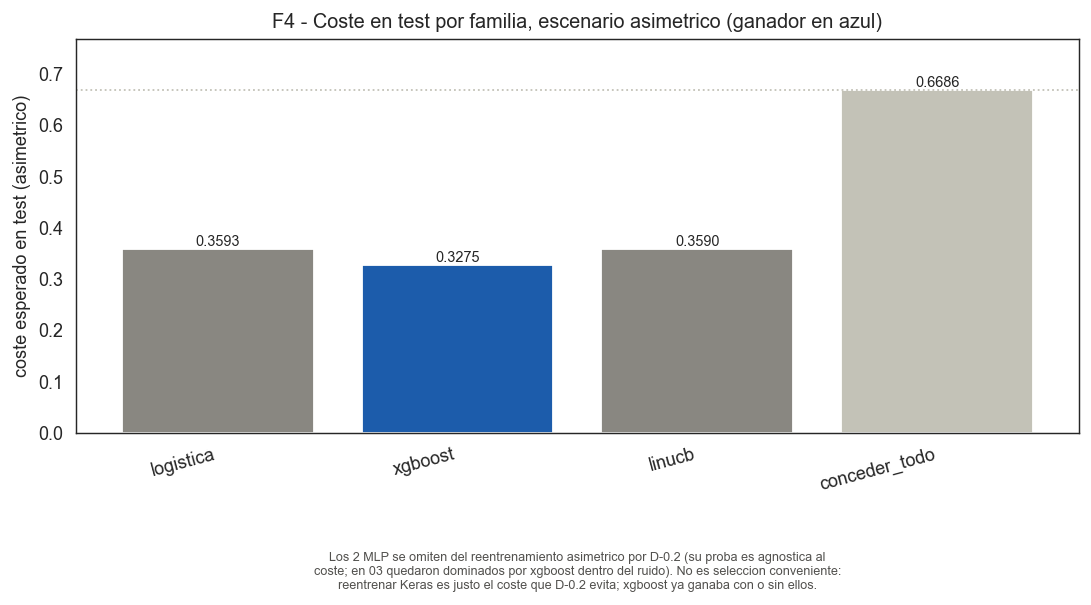
\includegraphics[width=.85\linewidth]{mod_04_comparacion_familias.png}
\caption{Coste por familia de modelo bajo el escenario asim\'etrico. A diferencia del
escenario sim\'etrico, aqu\'i la familia de modelo s\'i importa.}
\label{fig:mod04-comparacion-familias}
\end{figure}

A diferencia del escenario sim\'etrico --donde el margen entre familias era de solo
$\sim 0.0006$ y pr\'acticamente irrelevante--, bajo asimetr\'ia XGBoost (coste CV $=0.3344$)
supera a la regresi\'on log\'istica ($0.3513$) y al bandit LinUCB ($0.3502$) por un margen de
$0.0170$, un orden de magnitud mayor. El bandit LinUCB iguala aproximadamente a la
regresi\'on log\'istica (ambos de capacidad lineal), lo que indica que la ventaja de XGBoost
proviene de su mayor capacidad de modelado (boosting de \'arboles), no del mero hecho de ser
un m\'etodo supervisado frente a un bandit.

\subsection{Efecto sobre la matriz de confusi\'on y sobre la producci\'on}

Encarecer el falso negativo desplaza fuertemente el punto de operaci\'on del modelo hacia la
denegaci\'on preventiva (Figura~\ref{fig:mod04-confusion-contraste}). En el conjunto de test
(21\,000 solicitudes), los falsos negativos bajan de 1118 (escenario sim\'etrico) a
\textbf{396}, mientras que los falsos positivos suben de 213 a \textbf{2918}: el trasvase
exacto que impone penalizar diez veces m\'as conceder cr\'edito a un moroso. Con el umbral
asim\'etrico el modelo alcanza en test una precisi\'on de $0.2568$ y un recall de $0.7179$,
frente a $0.5731$ y $0.2037$ respectivamente en el escenario sim\'etrico. El \'Area Bajo la
Curva ROC (AUC) se mantiene id\'entica, $0.8701$, en ambos escenarios: es la prueba directa de
que solo cambia el punto de corte sobre la misma probabilidad estimada, no el modelo
subyacente.

\begin{figure}[H]
\centering
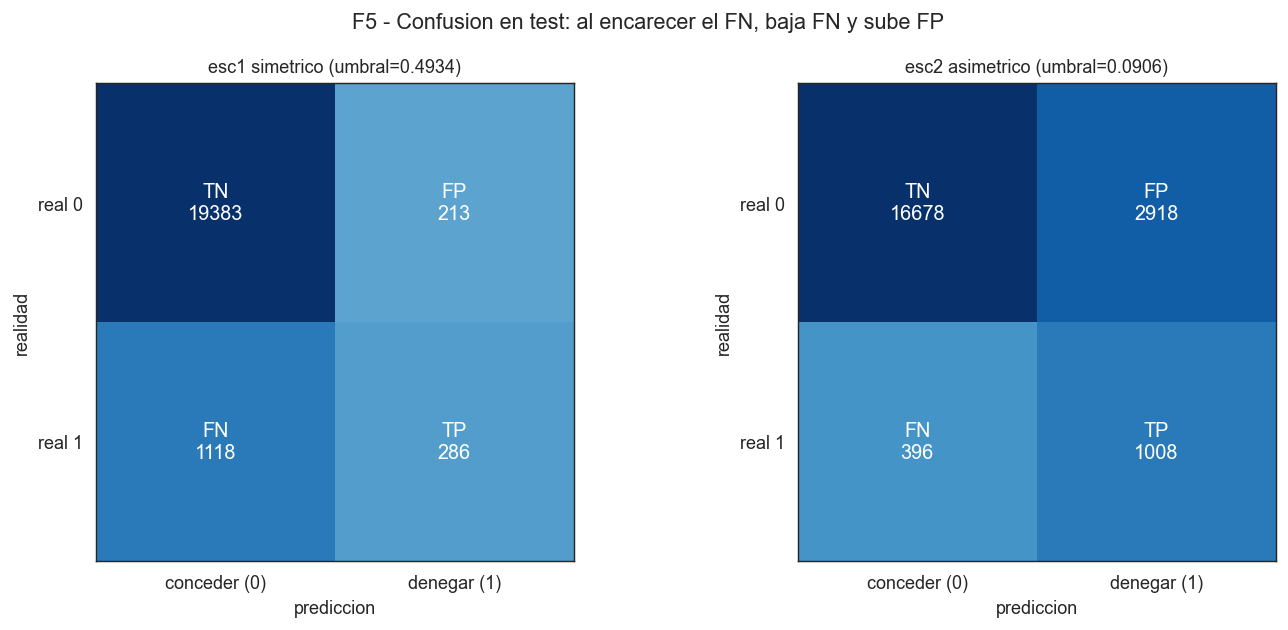
\includegraphics[width=.85\linewidth]{mod_04_confusion_contraste.png}
\caption{Matrices de confusi\'on en test, escenario sim\'etrico frente a escenario asim\'etrico:
los falsos negativos caen de 1118 a 396 y los falsos positivos suben de 213 a 2918.}
\label{fig:mod04-confusion-contraste}
\end{figure}

Consecuentemente, la tasa de denegaci\'on en test sube de $2.38\%$ a $18.70\%$. Aplicando el
mismo umbral asim\'etrico sobre las 45\,000 solicitudes del conjunto de producci\'on (sin
etiqueta observable), la tasa de denegaci\'on pasa de $2.36\%$ (1060 solicitantes) a
$18.53\%$ (8339 solicitantes): 7279 solicitantes cambian de concedido a denegado y ninguno en
sentido inverso, porque el umbral asim\'etrico es estrictamente m\'as bajo que el sim\'etrico
y, por construcci\'on, sus denegaciones incluyen a todas las del escenario sim\'etrico.

\subsection{Hallazgos}

\begin{itemize}
\item El umbral \'optimo emp\'irico ($0.0906$) casi coincide con el anal\'itico te\'orico
$1/11=0.0909$: el modelo est\'a bien calibrado justo en la banda de decisi\'on (probabilidad
predicha $\sim 0.0968$ frente a tasa real de impago $\sim 0.0996$ en el intervalo
$[0.08,0.12)$); adem\'as el m\'inimo de coste es plano, con solo $\sim 0.0008$ de diferencia
entre usar el umbral anal\'itico o el emp\'irico.
\item Bajo asimetr\'ia el modelo aporta un valor de negocio sustancialmente mayor: el coste
en test baja de $0.6686$ (conceder-todo) a $0.3275$, una mejora relativa del $51.01\%$, muy
por encima del $5.20\%$ logrado en el escenario sim\'etrico, y ambos muy por debajo del coste
de denegar-todo ($0.9331$).
\item Aqu\'i la familia de modelo s\'i importa: XGBoost (coste CV $=0.3344$) bate a la
regresi\'on log\'istica ($0.3513$) y al bandit LinUCB ($0.3502$) por un margen de $0.0170$,
muy superior al $\sim 0.0006$ que separaba a las familias en el escenario sim\'etrico; el
bandit iguala aproximadamente a la log\'istica (misma capacidad lineal), lo que sit\'ua la
ventaja de XGBoost en su capacidad de boosting y no en el paradigma supervisado \emph{per se}.
\item La matriz de confusi\'on en test se reequilibra al encarecer el falso negativo: los
falsos negativos bajan de 1118 a 396 y los falsos positivos suben de 213 a 2918; el modelo
ganador alcanza precisi\'on $=0.2568$, recall $=0.7179$ y AUC $=0.8701$ (el AUC no cambia
porque el scoring es el mismo; solo cambia el punto de corte).
\item La tasa de denegaci\'on sube de $2.38\%$ a $18.70\%$ en test y, aplicando el mismo
umbral en producci\'on, de $2.36\%$ (1060 de 45\,000) a $18.53\%$ (8339 de 45\,000): 7279
solicitantes pasan de concedido a denegado y ninguno en sentido inverso, consecuencia directa
de que el umbral asim\'etrico es estrictamente m\'as bajo que el sim\'etrico.
\end{itemize}

\section{Tabla comparativa de resultados entre ambos escenarios}

Esta sección consolida y contrasta, sobre el mismo conjunto de test reservado, los resultados de los dos
escenarios de coste desarrollados en las secciones anteriores: el escenario simétrico
($C_{FP}=C_{FN}=1$, Sección 5) y el escenario asimétrico ($C_{FP}=1$, $C_{FN}=10$, Sección 6), en el que
conceder crédito a un moroso -falso negativo- cuesta diez veces más que denegarlo a un buen pagador
-falso positivo-. El estimador subyacente es, en ambos casos, exactamente el mismo XGBoost entrenado una
única vez sobre las 84\,000 observaciones de entrenamiento; lo único que cambia entre escenarios es el
punto de corte $\theta$ que convierte la probabilidad de impago estimada en una decisión binaria
(conceder/denegar). En los dos escenarios el umbral se optimiza por validación cruzada estratificada de
5 pliegues sobre las probabilidades \emph{out-of-fold} (OOF) de \texttt{train}, nunca sobre \texttt{test},
que se reserva íntegro para el reporte final y se evalúa una única vez.

\subsection*{Metodología: umbral óptimo y coste esperado}

Bajo una matriz de coste asimétrica en la que el acierto no cuesta nada, el umbral de decisión que
minimiza el coste esperado de un clasificador binario bien calibrado tiene solución analítica cerrada:

\[
\theta^{*} = \frac{C_{FP}}{C_{FP}+C_{FN}}
\]

lo que da $\theta^{*}_{1} = \tfrac{1}{1+1} = 0.5000$ para el escenario simétrico y
$\theta^{*}_{10} = \tfrac{1}{1+10} = 0.0909$ para el asimétrico. El umbral empírico se obtiene por
búsqueda exhaustiva (\emph{argmin}) del coste medio sobre las probabilidades OOF de \texttt{train}, y el
coste esperado empírico sobre un conjunto de $N$ observaciones se calcula directamente a partir de la
matriz de confusión en el punto de corte elegido:

\[
\overline{\text{Coste}} = \frac{C_{FP}\cdot FP + C_{FN}\cdot FN}{N}
\]

Esta identidad es consistente con las cifras reportadas: en el escenario simétrico,
$(1\cdot 213 + 1\cdot 1118)/21\,000 = 0.0634$; en el asimétrico,
$(1\cdot 2918 + 10\cdot 396)/21\,000 = 0.3275$, ambos coincidentes con la columna
\texttt{coste\_test} de la Tabla~\ref{tab:comparativa-escenarios}.

\begin{figure}[H]
\centering
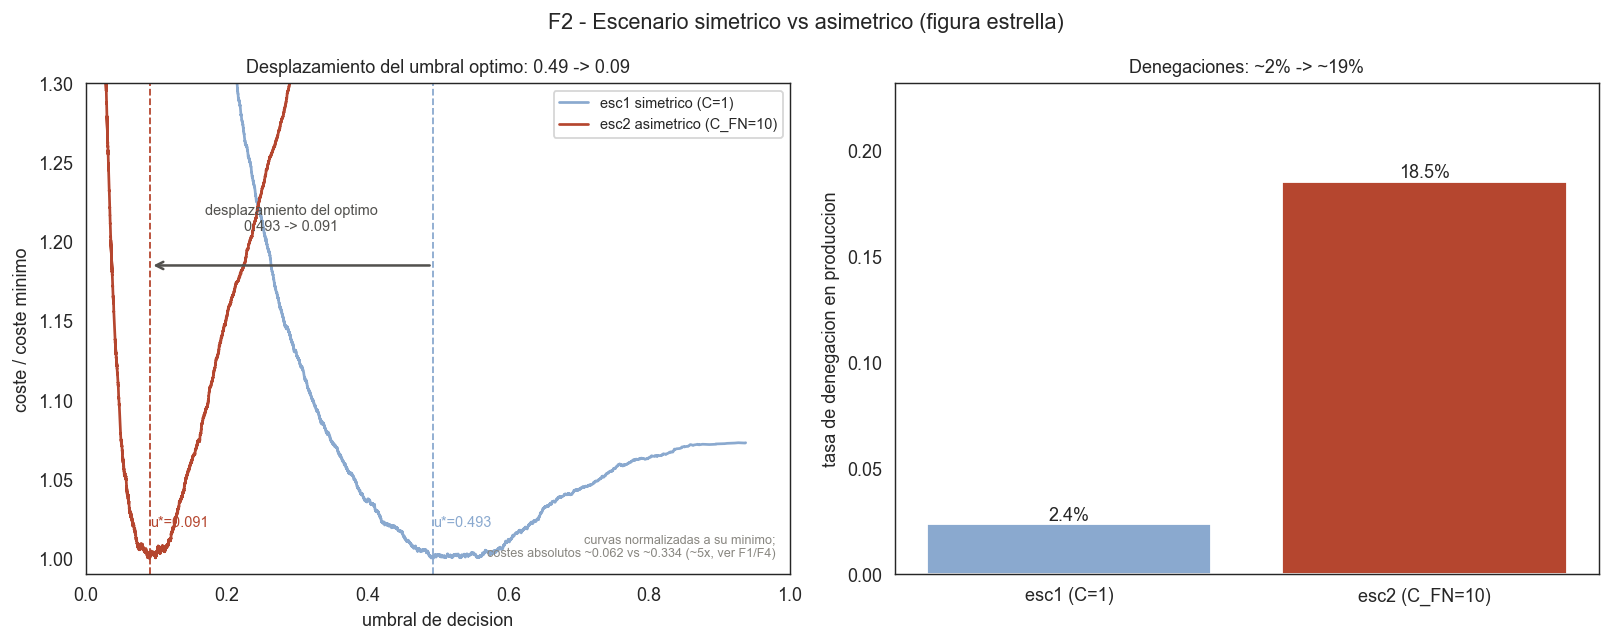
\includegraphics[width=.85\linewidth]{mod_04_comparacion_escenarios.png}
\caption{Comparación directa de los dos escenarios de coste sobre el mismo modelo XGBoost: umbral
óptimo, coste en test y tasa de denegación resultante en cada caso.}
\label{fig:comparacion-escenarios}
\end{figure}

\subsection*{Resultados comparados en test}

La Tabla~\ref{tab:comparativa-escenarios} recoge, para cada escenario, la familia de modelo ganadora,
el umbral óptimo empírico, el coste medio en \texttt{test}, el coste del baseline trivial de
\emph{conceder a todos} y la mejora relativa que logra el modelo umbralizado frente a ese baseline.

\begin{table}[H]
\centering
\caption{Comparativa de resultados en test entre el escenario simétrico y el asimétrico
(fuente: \texttt{umbrales\_coste.csv}).}
\label{tab:comparativa-escenarios}
\begin{tabular}{lccccc}
\toprule
Escenario & Umbral $\theta^{*}$ & Coste test & Coste conceder-todo & Denegación test & Mejora relativa \\
\midrule
Simétrico ($C_{FN}=1$)  & 0.4934 & 0.0634 & 0.0669 & 2.38\% & 5.20\% \\
Asimétrico ($C_{FN}=10$) & 0.0906 & 0.3275 & 0.6686 & 18.70\% & 51.01\% \\
\bottomrule
\end{tabular}
\end{table}

El coste del baseline de \emph{denegar a todos} es idéntico en ambos escenarios (0.9331), puesto que un
solicitante denegado nunca genera falso negativo y por tanto ese coste no depende de $C_{FN}$; en ambos
casos queda muy por encima del coste del modelo umbralizado, que domina a los dos baselines triviales.

\subsection*{Reequilibrio de la matriz de confusión}

Al mantenerse fijo el modelo y desplazarse únicamente el umbral, la matriz de confusión en test se
reequilibra de forma predecible: al encarecer diez veces el falso negativo, el modelo se vuelve mucho
más conservador a la hora de conceder crédito, lo que reduce los falsos negativos a costa de aumentar
los falsos positivos. La Tabla~\ref{tab:confusion-comparativa} cuantifica ese trasvase.

\begin{table}[H]
\centering
\caption{Falsos positivos, falsos negativos y métricas de contexto en test, mismo modelo, dos umbrales.}
\label{tab:confusion-comparativa}
\begin{tabular}{lccccc}
\toprule
Escenario & FP & FN & Precisión & Recall & AUC \\
\midrule
Simétrico ($\theta=0.4934$)  & 213  & 1118 & 0.5731 & 0.2037 & 0.8701 \\
Asimétrico ($\theta=0.0906$) & 2918 & 396  & 0.2568 & 0.7179 & 0.8701 \\
\bottomrule
\end{tabular}
\end{table}

El AUC de test es idéntico (0.8701) en los dos escenarios: es prueba cuantitativa directa de que se trata
del mismo modelo re-umbralizado y no de un reentrenamiento distinto, ya que el AUC es invariante al punto
de corte y solo depende del ordenamiento de las probabilidades predichas.

\begin{figure}[H]
\centering
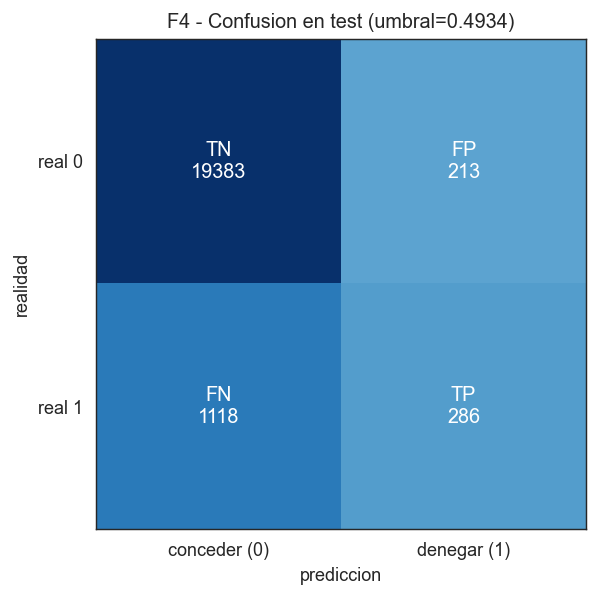
\includegraphics[width=.7\linewidth]{mod_03_confusion_optimo.png}
\caption{Matriz de confusión en test bajo el umbral óptimo del escenario simétrico ($\theta=0.4934$):
predominan los falsos negativos (1118) sobre los falsos positivos (213), coherente con un recall bajo.}
\label{fig:confusion-optimo}
\end{figure}

\begin{figure}[H]
\centering
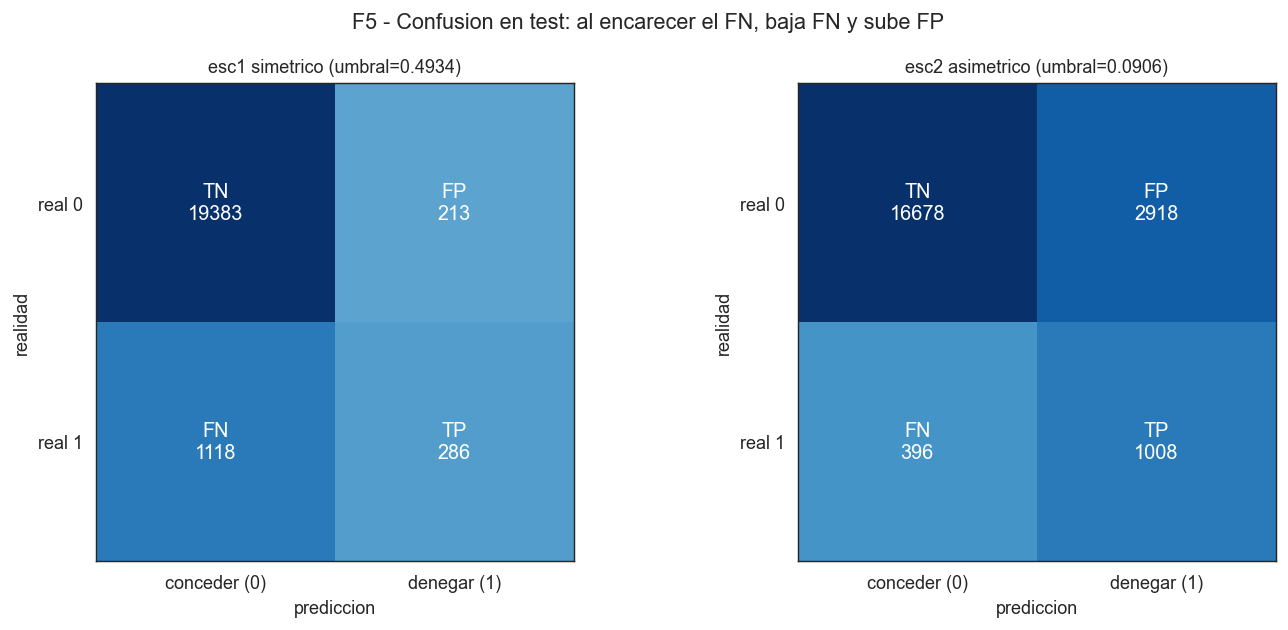
\includegraphics[width=.85\linewidth]{mod_04_confusion_contraste.png}
\caption{Contraste de matrices de confusión entre el umbral simétrico y el asimétrico: el trasvase de
falsos negativos hacia falsos positivos al bajar el umbral de 0.4934 a 0.0906.}
\label{fig:confusion-contraste}
\end{figure}

\subsection*{Tasa de denegación en test y en producción}

La tasa de denegación en test sube de 2.38\% (escenario simétrico) a 18.70\% (escenario asimétrico).
Como el objetivo de esta sección es comparar los dos escenarios de negocio y las etiquetas reales de
producción permanecen ocultas -su evaluación final corresponde al profesor-, se emplea como proxy
observable la tasa de denegación en producción, calculada directamente sobre la columna de decisión
\emph{predicha} (0 = concedido, 1 = denegado) que el modelo escribe en cada fichero de entrega, sin
requerir el target oculto. La Tabla~\ref{tab:denegacion-produccion} resume el resultado sobre las
45\,000 solicitudes de cada fichero de producción.

\begin{table}[H]
\centering
\caption{Tasa de denegación en producción según el fichero de entrega (45\,000 solicitudes cada uno).}
\label{tab:denegacion-produccion}
\begin{tabular}{lccc}
\toprule
Escenario & Fichero & Denegados & Tasa de denegación \\
\midrule
Simétrico  & \texttt{cs\_produccion1.csv} & 1060 & 2.36\% \\
Asimétrico & \texttt{cs\_produccion2.csv} & 8339 & 18.53\% \\
\bottomrule
\end{tabular}
\end{table}

Puesto que el umbral asimétrico ($\theta=0.0906$) es estrictamente inferior al simétrico
($\theta=0.4934$), su conjunto de denegados es un superconjunto del anterior: aplicando el mismo scoring
a las 45\,000 solicitudes de producción, 7279 solicitantes (16.2\% del total) pasan de concedido a
denegado al endurecer el criterio, y ninguno lo hace en sentido inverso.

\subsection*{Hallazgos}

\begin{itemize}
\item El AUC de test es idéntico en los dos escenarios (0.8701): prueba cuantitativa de que es el mismo
modelo re-umbralizado y no un reentrenamiento distinto. El umbral óptimo empírico cae de 0.4934
(simétrico) a 0.0906 (asimétrico), ambos muy próximos a sus umbrales analíticos teóricos
($\theta^{*}_{1}=0.5$ y $\theta^{*}_{10}=1/11=0.0909$): el scoring está bien calibrado en la zona de
decisión relevante.
\item El equilibrio FP/FN se invierte con fuerza al pasar del escenario simétrico al asimétrico: los
falsos negativos caen de 1118 a 396 y los falsos positivos suben de 213 a 2918 (recall
$0.2037\rightarrow 0.7179$, precisión $0.5731\rightarrow 0.2568$); el modelo se vuelve mucho más
conservador a la hora de conceder crédito cuando el impago no detectado cuesta diez veces más.
\item La mejora relativa frente al baseline de conceder-a-todos escala fuertemente con la asimetría:
5.20\% en el escenario simétrico frente a 51.01\% en el asimétrico, con la misma familia ganadora
(\texttt{xgboost}) en ambos casos; el coste de denegar-a-todos es idéntico en los dos escenarios
(0.9331) porque no depende de $C_{FN}$.
\item La tasa de denegación en test sube de 2.38\% a 18.70\%; en producción el patrón se repite de forma
casi idéntica (2.36\% frente a 18.53\% sobre 45\,000 solicitudes), calculada sobre la decisión predicha
por el modelo, no sobre una etiqueta real, lo que permite reportarla sin conocer el target oculto.
\item Del escenario simétrico al asimétrico, 7279 de los 45\,000 solicitantes de producción (16.2\%)
pasan de concedido a denegado, y ninguno en sentido inverso: al ser el umbral asimétrico estrictamente
más bajo, sus denegados incluyen a todos los del escenario simétrico más los nuevos casos límite que
quedan por debajo del nuevo corte.
\end{itemize}

\section{Auditoría: modelo subrogado con reglas}

\subsection{Metodología: fidelidad frente a exactitud}

Para auditar el comportamiento del modelo de caja negra (XGBoost) se entrena, para cada escenario de coste, un árbol de decisión (\texttt{DecisionTreeClassifier}) que \textbf{no} predice el impago real: imita la \emph{decisión} que XGBoost toma (conceder o denegar) una vez aplicado el umbral de coste correspondiente. Recordemos que dicha decisión surge de comparar la probabilidad de impago estimada con el umbral óptimo de cada escenario, obtenido por búsqueda exhaustiva sobre las probabilidades OOF de train y próximo al óptimo analítico
\[
\theta^{*} = \frac{C_{FP}}{C_{FP}+C_{FN}},
\]
con $\theta^{*}_{\text{coste1}}=0.4934$ (analítico $0.5$) y $\theta^{*}_{\text{coste10}}=0.0906$ (analítico $1/11=0.0909$).

Por construcción, el árbol subrogado se evalúa por \textbf{fidelidad} respecto a la caja negra, no por exactitud frente al impago verdadero. Sea $n$ el número de observaciones de test, $\hat y_i^{\text{caja}}\in\{0,1\}$ la decisión de XGBoost + umbral (1 = denegar) y $\hat y_i^{\text{sub}}\in\{0,1\}$ la decisión del árbol subrogado para la observación $i$. Se definen:

\begin{align}
F_{\text{global}} &= \frac{1}{n}\sum_{i=1}^{n} \mathbf{1}\!\left[\hat y_i^{\text{sub}} = \hat y_i^{\text{caja}}\right] \\
F_{\text{denegar}} &= \frac{\sum_{i=1}^{n} \mathbf{1}\!\left[\hat y_i^{\text{sub}}=1 \,\wedge\, \hat y_i^{\text{caja}}=1\right]}{\sum_{i=1}^{n} \mathbf{1}\!\left[\hat y_i^{\text{caja}}=1\right]}
\end{align}

$F_{\text{global}}$ es la proporción de observaciones en las que el subrogado reproduce la decisión de la caja negra; $F_{\text{denegar}}$ es el recall del subrogado sobre la clase \emph{denegar} tomando como referencia la propia caja negra (no el impago real). El $F1_{\text{denegar}}$ se calcula como la media armónica de precisión y $F_{\text{denegar}}$, ambas respecto a la etiqueta de la caja negra.

Esta distinción es crítica bajo el fuerte desbalanceo de decisiones del escenario simétrico (solo el $2.38\%$ de test es denegado): un árbol degenerado que concediera siempre alcanzaría $F_{\text{global}}=0.9762$ sin haber aprendido ningún patrón de denegación ($F_{\text{denegar}}=0$). Por ello se barre la profundidad del árbol (de 2 a 10) y el peso asignado a la clase \emph{denegar}, observando siempre la fidelidad de la clase rara y no solo la global.

\begin{figure}[H]
\centering
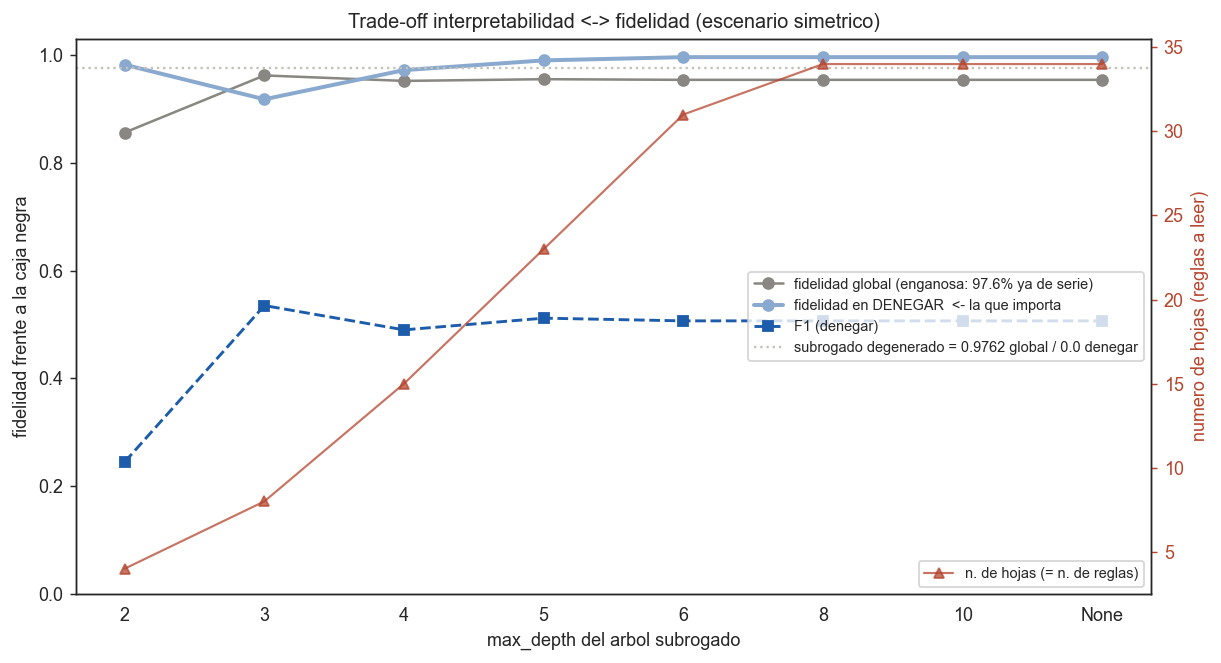
\includegraphics[width=.85\linewidth]{sub_05_fidelidad_vs_profundidad_coste1.png}
\caption{Fidelidad global, fidelidad de la clase denegar y $F1$-denegar en función de la profundidad del árbol y del peso de clase, escenario coste1. La fidelidad global satura casi plana cerca de $0.98$ desde poca profundidad, mientras que la fidelidad de la clase denegar sigue mejorando con la profundidad y depende fuertemente del peso de clase: ahí reside el verdadero límite de aprendizaje del subrogado.}
\label{fig:sub-fidelidad-profundidad}
\end{figure}

A partir de este barrido se fijan, para cada escenario, dos árboles con propósitos distintos:

\begin{itemize}
\item \textbf{Árbol operativo} (profundidad 5, 23 hojas): maximiza la fidelidad y se emplea para la auditoría técnica del modelo.
\item \textbf{Árbol de bolsillo} (profundidad 3, 8 hojas): legible de un vistazo, pensado para comunicar la lógica de decisión a un cliente o a un revisor no técnico.
\end{itemize}

Los umbrales de las reglas resultantes se traducen a euros, años y ratios reales (no a la escala estandarizada interna del pipeline) invirtiendo las transformaciones de \texttt{PreprocesadorCredito} (winsorizado, $\log(1+x)$ y escalado).

\subsection{Los dos árboles de bolsillo: dos personalidades de riesgo}

\begin{figure}[H]
\centering
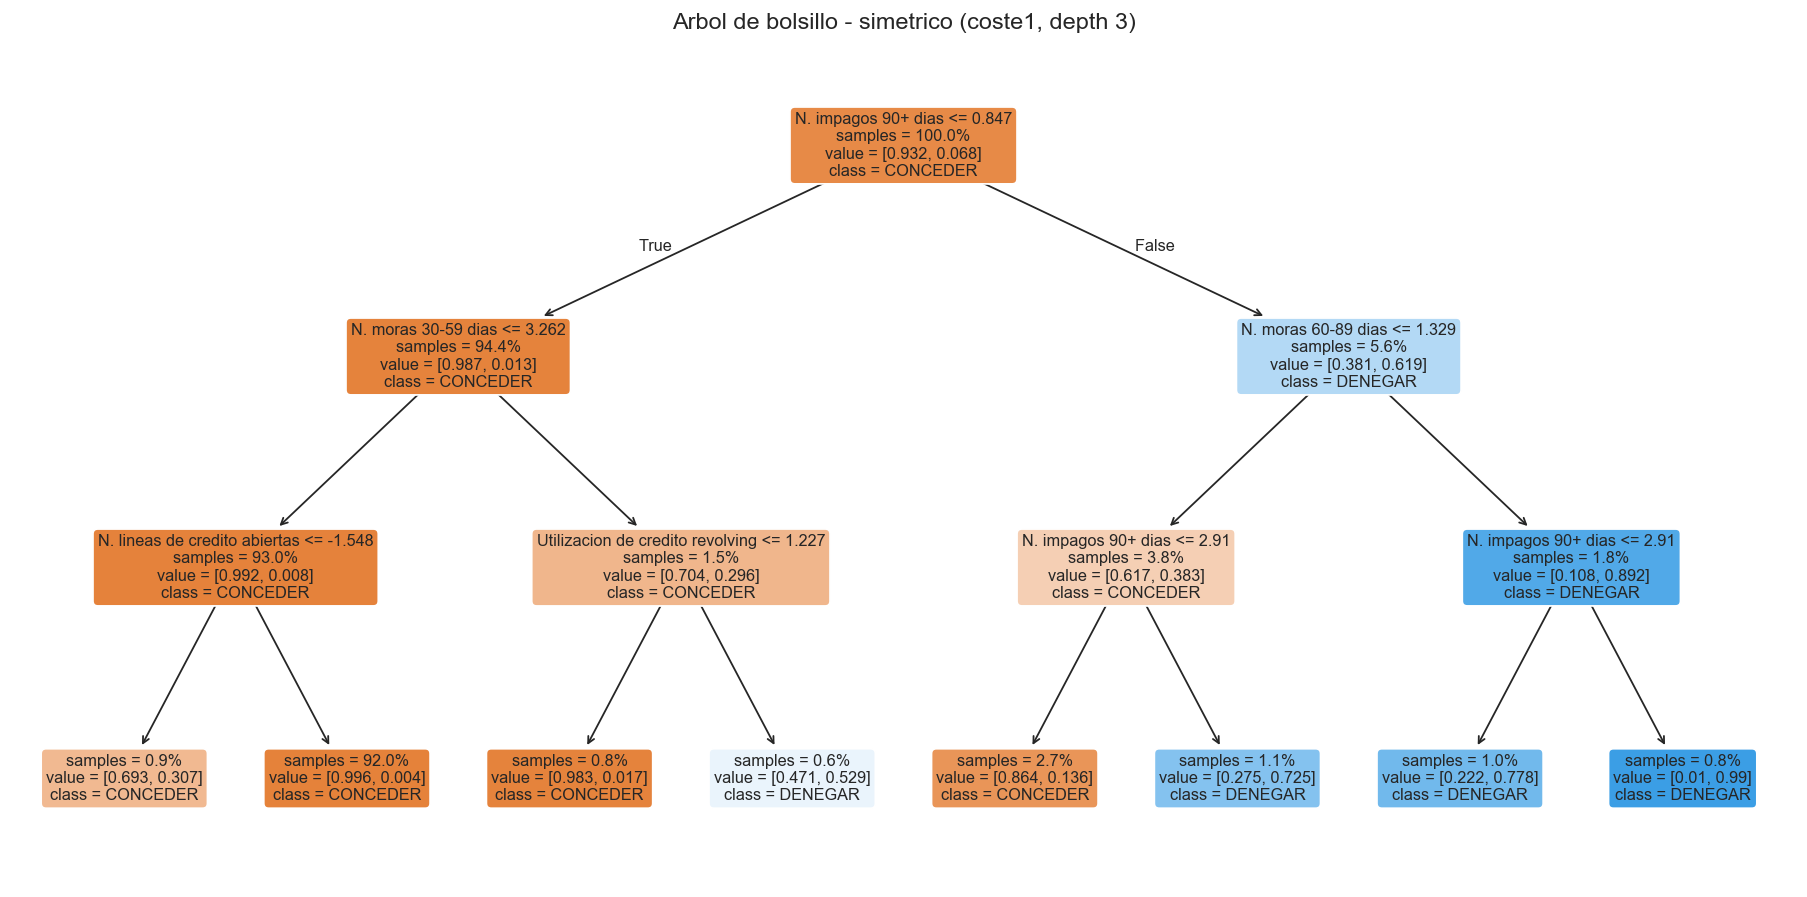
\includegraphics[width=.7\linewidth]{sub_05_arbol_bolsillo_coste1.png}
\caption{Árbol de bolsillo del escenario coste1 (umbral $0.4934$, deniega al $2.38\%$ de los solicitantes). La variable de la raíz es el número de impagos de 90 o más días: un criterio conservador basado en mora ya consumada.}
\label{fig:sub-bolsillo-coste1}
\end{figure}

\begin{figure}[H]
\centering
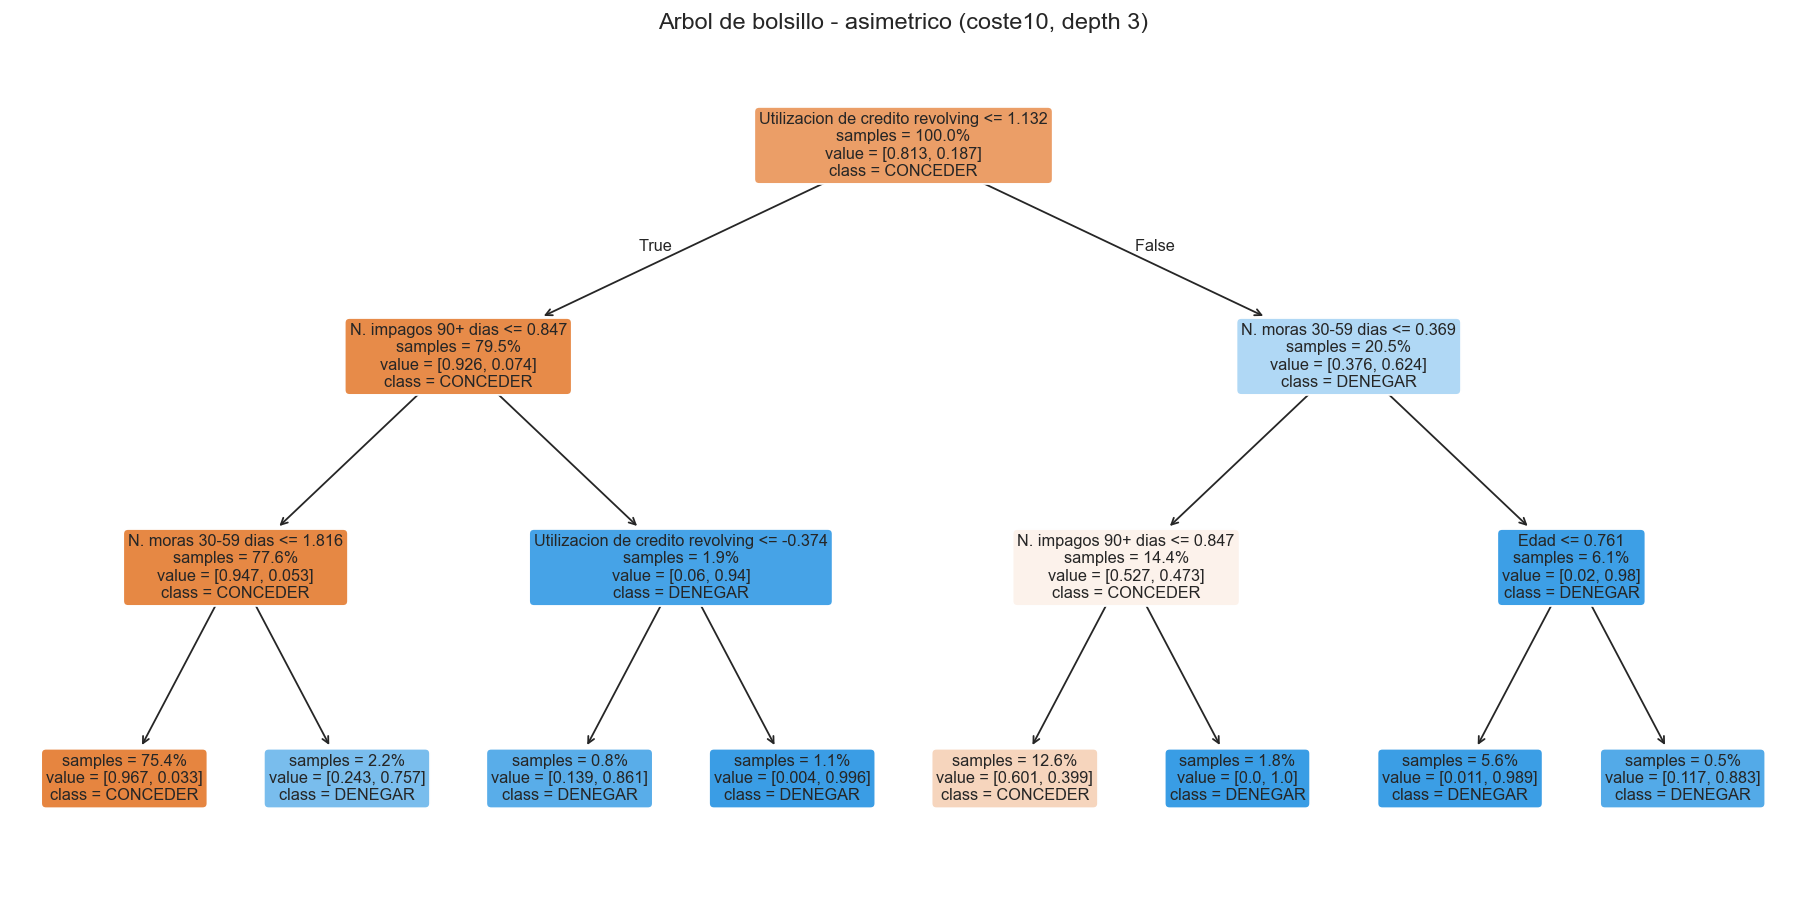
\includegraphics[width=.7\linewidth]{sub_05_arbol_bolsillo_coste10.png}
\caption{Árbol de bolsillo del escenario coste10 (umbral $0.0906$, deniega al $18.70\%$ de los solicitantes). La variable de la raíz es la utilización de crédito revolving: un criterio preventivo basado en una señal de estrés financiero temprano.}
\label{fig:sub-bolsillo-coste10}
\end{figure}

Ambos árboles provienen del mismo XGBoost; la única diferencia es el umbral de coste aplicado aguas abajo. Aun así, la variable que ocupa la raíz del árbol de bolsillo se invierte por completo entre escenarios, lo que anticipa el resultado de importancia de variables de la Sección~\ref{sec:sub-importancia}.

\begin{figure}[H]
\centering
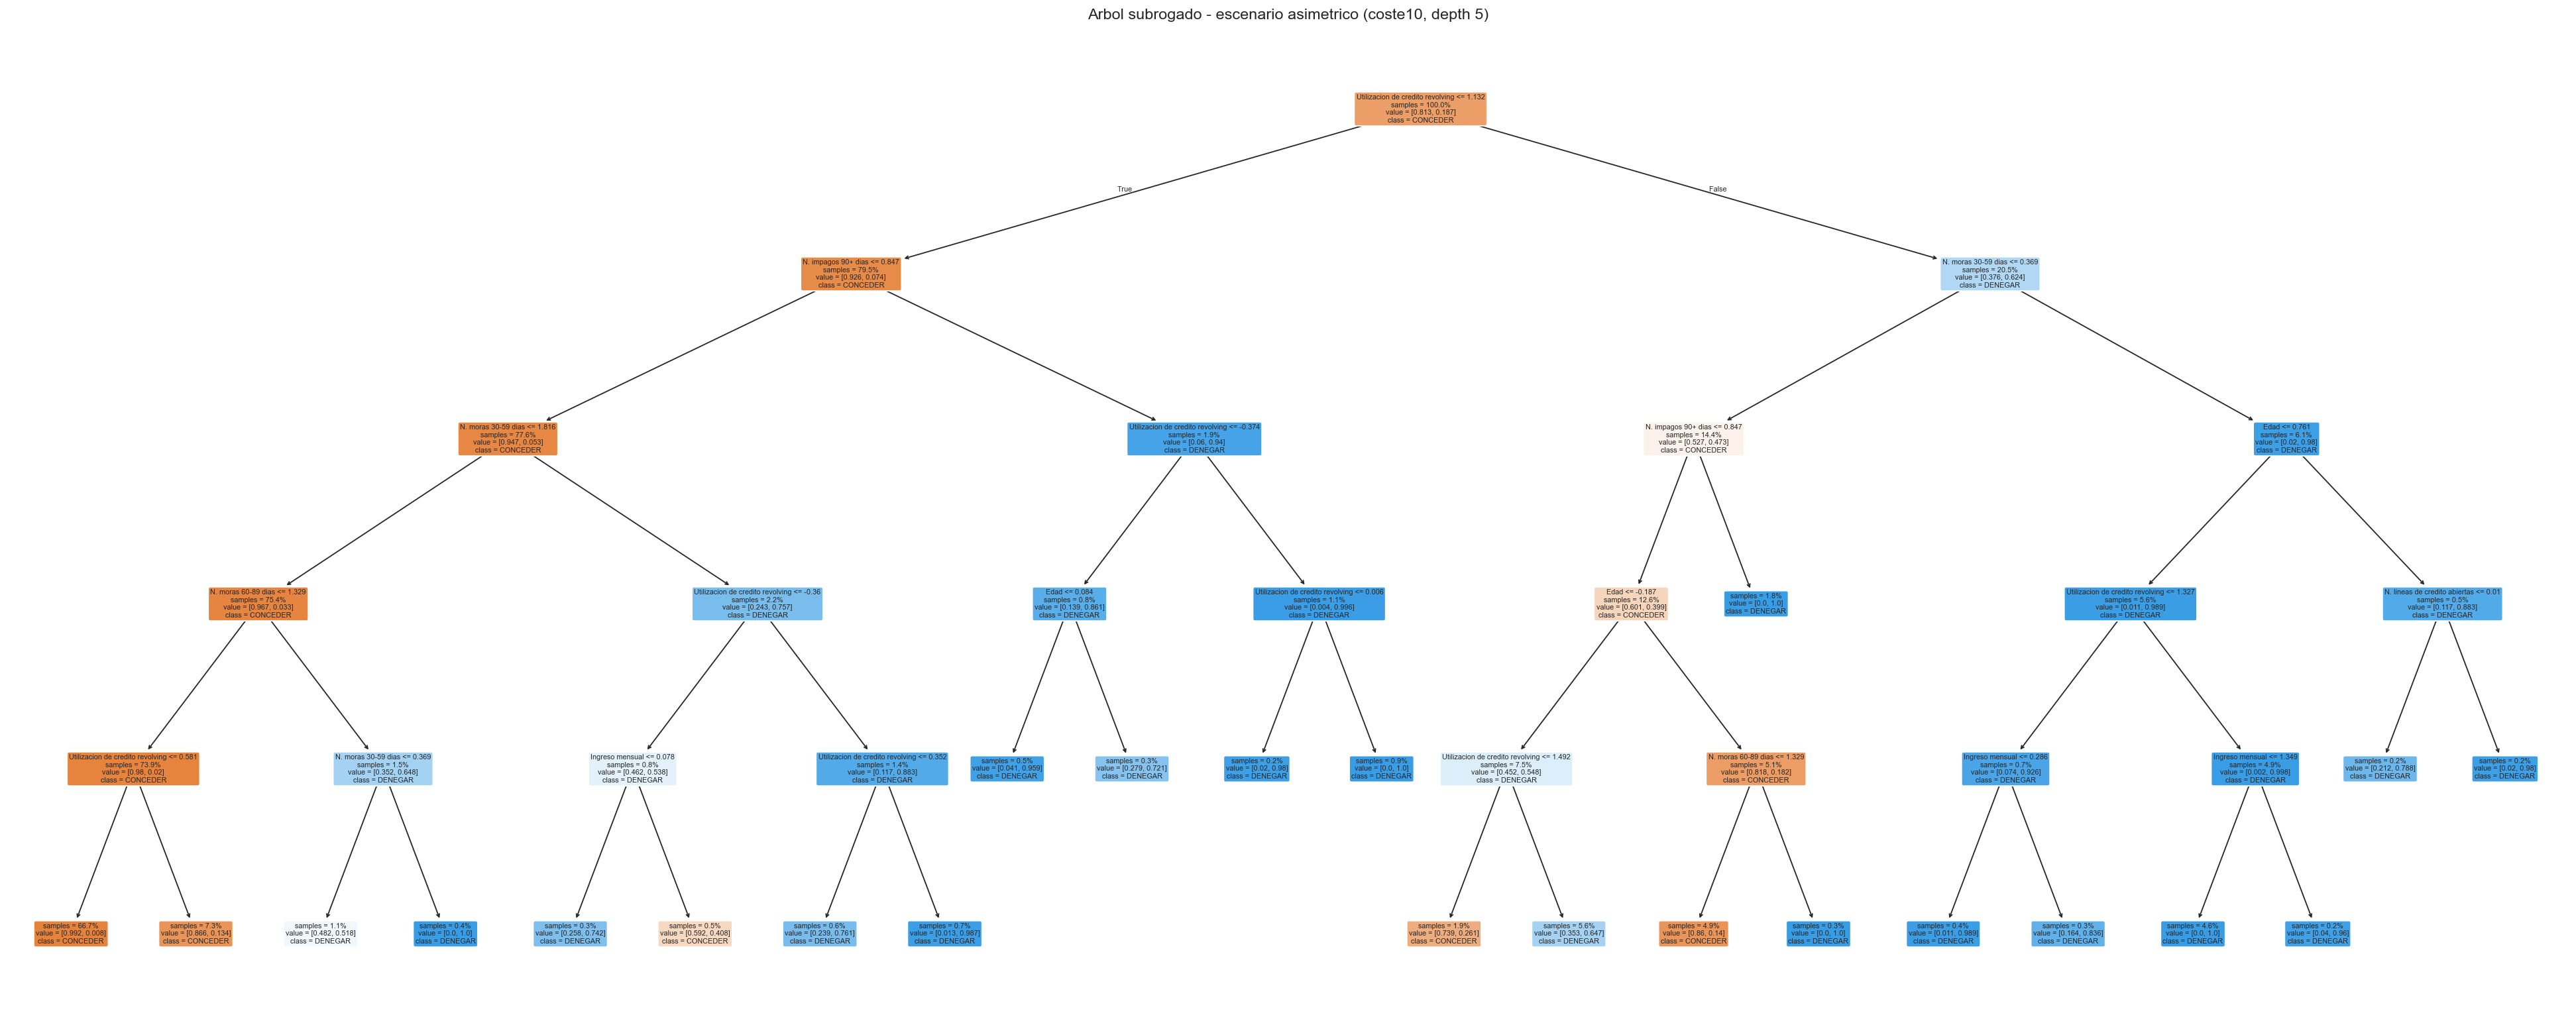
\includegraphics[width=.9\linewidth]{arbol_subrogado_coste10.png}
\caption{Árbol operativo completo (23 hojas) del escenario coste10. Con mayor profundidad se despliega la jerarquía completa de la variable dominante (utilización de crédito revolving) combinada con variables de mora y edad; de estas ramas se extraen, una por una, las reglas de denegación listadas en la Sección~\ref{sec:sub-reglas}.}
\label{fig:sub-arbol-operativo-coste10}
\end{figure}

\subsection{Fidelidad de los cuatro subrogados fijados}

La Tabla~\ref{tab:sub-fidelidad} recoge la fidelidad de los cuatro árboles fijados (operativo y bolsillo, en cada escenario), junto con la tasa de denegación real de la caja negra y la que reproduce cada subrogado, como chequeo de sanidad independiente de las métricas de fidelidad.

\begin{table}[H]
\centering
\footnotesize
\caption{Fidelidad de los subrogados frente a la caja negra (XGBoost + umbral de coste) en test.}
\label{tab:sub-fidelidad}
\begin{tabular}{lrrrrrr}
\toprule
Subrogado & Hojas & Denegación caja negra & Denegación subrogado & Fidelidad global & Fidelidad denegar & $F1$ denegar \\
\midrule
Coste1 operativo (d=5) & 23 & 0.0238 & 0.0259 & 0.9879 & 0.7896 & 0.7562 \\
Coste1 bolsillo (d=3) & 8 & 0.0238 & 0.0353 & 0.9809 & 0.8397 & 0.6758 \\
Coste10 operativo (d=5) & 23 & 0.1870 & 0.1876 & 0.9415 & 0.8454 & 0.8439 \\
Coste10 bolsillo (d=3) & 8 & 0.1870 & 0.1196 & 0.9173 & 0.5988 & 0.7304 \\
\bottomrule
\end{tabular}
\end{table}

En los cuatro casos la tasa de denegación reproducida por el subrogado se aproxima a la de la caja negra ($0.0259$ vs.\ $0.0238$ en coste1 operativo; $0.1876$ vs.\ $0.1870$ en coste10 operativo), lo que confirma que el árbol no solo clasifica bien en promedio, sino que replica el volumen real de decisiones adversas.

\subsection{Importancia de variables en cada subrogado}
\label{sec:sub-importancia}

La Tabla~\ref{tab:sub-importancia} muestra la importancia de variables (basada en la reducción de impureza) del árbol operativo de cada escenario.

\begin{table}[H]
\centering
\caption{Importancia de variables del árbol subrogado operativo, por escenario de coste.}
\label{tab:sub-importancia}
\begin{tabular}{lrr}
\toprule
Variable & Importancia coste1 & Importancia coste10 \\
\midrule
N.\ impagos 90+ días & 0.7155 & 0.1875 \\
N.\ moras 60--89 días & 0.1219 & 0.0685 \\
N.\ moras 30--59 días & 0.0734 & 0.2105 \\
Utilización de crédito revolving & 0.0397 & 0.4914 \\
N.\ líneas de crédito abiertas & 0.0208 & 0.0004 \\
Edad & 0.0165 & 0.0392 \\
Ratio de deuda & 0.0089 & 0.0000 \\
Ingreso mensual & 0.0032 & 0.0024 \\
\bottomrule
\end{tabular}
\end{table}

La variable dominante se invierte entre escenarios: en coste1 domina el número de impagos de 90 o más días (importancia $0.7155$), coherente con un modelo conservador que solo deniega ante mora ya consumada; en coste10 domina la utilización de crédito revolving (importancia $0.4914$), coherente con un modelo preventivo que deniega ante la primera señal de estrés financiero, mientras que los impagos de 90+ días caen al tercer puesto ($0.1875$).

\subsection{Reglas de denegación destiladas}
\label{sec:sub-reglas}

De las ramas del árbol operativo de 23 hojas que terminan en \emph{denegar} se extraen reglas legibles, con umbrales ya expresados en euros, años y ratios reales:

\begin{itemize}
\item \textbf{Coste1:} 8 reglas cubren 543 de las denegaciones de test. La regla principal (soporte 118, pureza $100\%$) deniega si el número de impagos de 90 o más días es $\geq 2$, el número de moras de 60--89 días es $\geq 2$ y la utilización de crédito revolving supera el $91\%$.
\item \textbf{Coste10:} 18 reglas cubren 3\,940 de las denegaciones de test. La regla principal (soporte 975, pureza $100\%$) deniega si la utilización de crédito revolving supera el $77\%$, el número de moras de 30--59 días es $\geq 2$, la edad es $\leq 63.5$ años y el ingreso mensual es $\leq 12\,506.50$ EUR.
\item \textbf{Interacción edad $\times$ mora (coste1):} dentro del subconjunto con impagos de 90+ días $\geq 2$ y moras de 60--89 días $\leq 1$, con moras de 30--59 días $\geq 2$, el corte de edad separa claramente el riesgo: edad $> 43.5$ años da pureza $75.0\%$ (soporte 58) frente a edad $\leq 43.5$ años con pureza $98.0\%$ (soporte 53). Esta interacción se corrobora de forma independiente con el PDP bidimensional presentado en la sección de otras técnicas de explicabilidad del notebook.
\end{itemize}

\subsection{Hallazgos}

\begin{itemize}
\item La fidelidad global engaña bajo desbalanceo: en coste1, el árbol degenerado que \emph{concede siempre} alcanza $F_{\text{global}}=0.9762$ con $F_{\text{denegar}}=0$ (no aprendió ningún patrón de denegación); el árbol operativo real eleva el global a $0.9879$ \textbf{y además} la fidelidad de la clase denegar a $0.7896$ ($F1_{\text{denegar}}=0.7562$). Debe examinarse siempre la fidelidad de la clase rara, nunca la global de forma aislada.
\item El peso óptimo de la clase \emph{denegar} depende del escenario: 3 en coste1 (clase rara, $2.38\%$ de denegaciones) frente a sin reponderar en coste10 (clase frecuente, $18.70\%$); en ambos casos el árbol operativo reproduce casi con exactitud la tasa de denegación real de la caja negra ($2.59\%$ vs.\ $2.38\%$ en coste1; $18.76\%$ vs.\ $18.70\%$ en coste10), un chequeo de sanidad independiente del $F1$.
\item Se identifican dos personalidades de riesgo: la variable más importante se invierte entre escenarios. En coste1 domina el número de impagos de 90+ días (importancia $0.7155$), un modelo conservador que solo deniega ante mora ya consumada; en coste10 domina la utilización de crédito revolving (importancia $0.4914$), un modelo preventivo que deniega ante la primera señal de estrés, con los impagos de 90+ días relegados al tercer puesto ($0.1875$). Mismo XGBoost, misma pareja de árboles, lógica de decisión opuesta según dónde se fija el umbral de coste.
\item El árbol de bolsillo (8 hojas) tiene un $F1$ más bajo en coste1 ($0.6758$) que en coste10 ($0.7304$), pero en cobertura el orden se invierte: cubre el $83.97\%$ de las denegaciones reales en coste1 frente a solo el $59.88\%$ en coste10. El bolsillo asimétrico es muy preciso pero con poca profundidad: 8 hojas son un techo estructural que en coste10 deja fuera a 4 de cada 10 denegaciones.
\item La brecha entre el árbol operativo y el de bolsillo en $F1$ es mayor en coste10 ($0.8439$ frente a $0.7304$, diferencia $-0.1135$) que en coste1 ($0.7562$ frente a $0.6758$, diferencia $-0.0804$): con más denegaciones que cubrir ($18.70\%$ frente a $2.38\%$), 8 reglas resultan insuficientes antes.
\end{itemize}

\paragraph{Nota de reproducibilidad.} Al recargar el XGBoost serializado (\texttt{.joblib}) con una versión de la librería distinta a la usada en el entrenamiento, el parámetro interno \texttt{base\_score} se reconstruía de forma incorrecta e inflaba las probabilidades por un factor de aproximadamente 5 (denegaría al $25\%$ / $85\%$ de los solicitantes en vez del $2.4\%$ / $18.7\%$ real). El problema se detectó y corrigió fijando la versión exacta de XGBoost en las dependencias antes de ejecutar esta auditoría, garantizando que todas las cifras anteriores correspondan al modelo realmente entrenado.

\section{Auditoría: análisis de contrafactuales}

\paragraph{Objetivo y metodología.} Un contrafactual responde a la pregunta \emph{¿qué habría tenido que cambiar el solicitante para que el modelo concediera el crédito?}. Formalmente, dado el clasificador $f:\mathcal{X}\rightarrow[0,1]$ que estima $p(\text{impago}\mid x)$ y la regla de decisión de negocio
\[
\hat{y}(x) = \mathbf{1}\left[f(x) \geq \theta\right],
\]
con $\theta$ el umbral operativo de cada escenario ($\theta=0{,}4934$ en coste1, $\theta=0{,}0906$ en coste10; véanse las secciones 5 y 6), un contrafactual accionable para una instancia denegada $x$ (con $f(x)\geq\theta$) es una instancia $x'$ que invierte la decisión, $f(x') < \theta$, modificando únicamente un subconjunto acotado de variables accionables.

La búsqueda se realiza con la librería DiCE (\emph{Diverse Counterfactual Explanations}), cuya frontera interna de decisión está fijada de fábrica en $0{,}5$. Como los umbrales de negocio reales ($0{,}4934$ y $0{,}0906$) no coinciden con esa frontera, se interpone un modelo adaptador que traslada la frontera interna de DiCE al umbral de negocio real de cada escenario. Así, la optimización de DiCE persigue siempre la decisión de negocio realmente aplicada por el banco en cada escenario, y no una frontera genérica al $50\%$.

La búsqueda se restringe a cuatro variables accionables --utilización de crédito revolving, ratio de deuda (\texttt{DebtRatio}), ingresos mensuales y número de líneas de crédito abiertas--, con límites de cambio realistas por solicitante:
\[
x'_{\text{ingresos}} \leq 1{,}25\, x_{\text{ingresos}}, \qquad
x'_{\text{revolving}} \geq 0{,}70\, x_{\text{revolving}}, \qquad
x'_{\text{DebtRatio}} \geq 0{,}70\, x_{\text{DebtRatio}}, \qquad
x'_{\text{lineas}} \geq x_{\text{lineas}} - 2 .
\]
El resto de variables (edad, historial de impagos, personas dependientes, etc.) permanece fijo. Cada candidato generado por DiCE se somete a seis comprobaciones antes de traducirse a una explicación para el cliente: (1) rango observado en los datos, (2) ausencia de valores negativos, (3) las variables inmutables no cambian, (4) el cambio va en la dirección favorable al solicitante, (5) las variables de conteo entero conservan valores enteros y (6) la decisión realmente se invierte bajo el umbral de negocio.

\paragraph{Selección de casos.} Se seleccionan 8 solicitudes denegadas: 2 por clase real ($0$/$1$) $\times$ 2 escenarios de coste (coste1, coste10), etiquetadas como \texttt{borde\_umbral} (la más cercana al umbral) o \texttt{denegacion\_fuerte} ($p(\text{impago})$ más alta). La clase real del solicitante determina el uso legítimo del contrafactual: si en realidad no habría impagado (falso positivo del modelo, \texttt{clase\_real=0}), el contrafactual es una explicación literal comunicable al cliente (\texttt{uso\_explicacion = explicacion\_cliente\_falso\_positivo}); si el modelo acertó al denegar (\texttt{clase\_real=1}), el contrafactual solo tiene valor de auditoría interna del comportamiento del modelo y no debe presentarse como promesa de aprobación (\texttt{uso\_explicacion = auditoria\_interna\_denegacion\_correcta}).

\subsection{Resultado principal}

De las 8 solicitudes analizadas, DiCE genera un contrafactual accionable en los 4 casos \texttt{borde\_umbral} (4/4) y en ninguno de los 4 casos \texttt{denegacion\_fuerte} (0/4): la distancia al umbral condiciona por completo la existencia de una explicación accionable, no la clase real del solicitante. De los 4 generados, 3 resultan plausibles tras las seis comprobaciones: $2/2$ en coste1 y $1/2$ en coste10.

\begin{table}[H]
\centering
\caption{Resultado del análisis de contrafactuales por caso (8 solicitudes denegadas).}
\label{tab:cf_ejemplos}
\begin{tabular}{lccllc}
\toprule
\texttt{id\_test} & escenario & clase\_real & tipo\_caso & estado\_cf & plausible \\
\midrule
52346 & coste1  & 0 & \texttt{borde\_umbral}      & generado             & sí \\
28495 & coste1  & 0 & \texttt{denegacion\_fuerte} & \texttt{sin\_cf\_accionable} & no \\
10358 & coste1  & 1 & \texttt{borde\_umbral}      & generado             & sí \\
79585 & coste1  & 1 & \texttt{denegacion\_fuerte} & \texttt{sin\_cf\_accionable} & no \\
19744 & coste10 & 0 & \texttt{borde\_umbral}      & generado             & sí \\
28495 & coste10 & 0 & \texttt{denegacion\_fuerte} & \texttt{sin\_cf\_accionable} & no \\
14183 & coste10 & 1 & \texttt{borde\_umbral}      & generado             & no \\
79585 & coste10 & 1 & \texttt{denegacion\_fuerte} & \texttt{sin\_cf\_accionable} & no \\
\bottomrule
\end{tabular}
\end{table}

\begin{table}[H]
\centering
\caption{Resumen por escenario: probabilidad de impago media de los 4 casos seleccionados, contrafactuales generados y plausibles.}
\label{tab:cf_resumen}
\begin{tabular}{lrrr}
\toprule
Escenario & $p(\text{impago})$ media & Generados & Plausibles \\
\midrule
coste1  & 0{,}6843 & 2 & 2 \\
coste10 & 0{,}4829 & 2 & 1 \\
\bottomrule
\end{tabular}
\end{table}

La probabilidad de impago media resume qué tan lejos del umbral están, en promedio, los 4 casos de cada escenario ($0{,}6843$ en coste1 frente a $0{,}4829$ en coste10); en términos absolutos, ambos grupos mezclan casos \texttt{borde\_umbral} con casos \texttt{denegacion\_fuerte}, muy por encima del corte.

\begin{figure}[H]
\centering
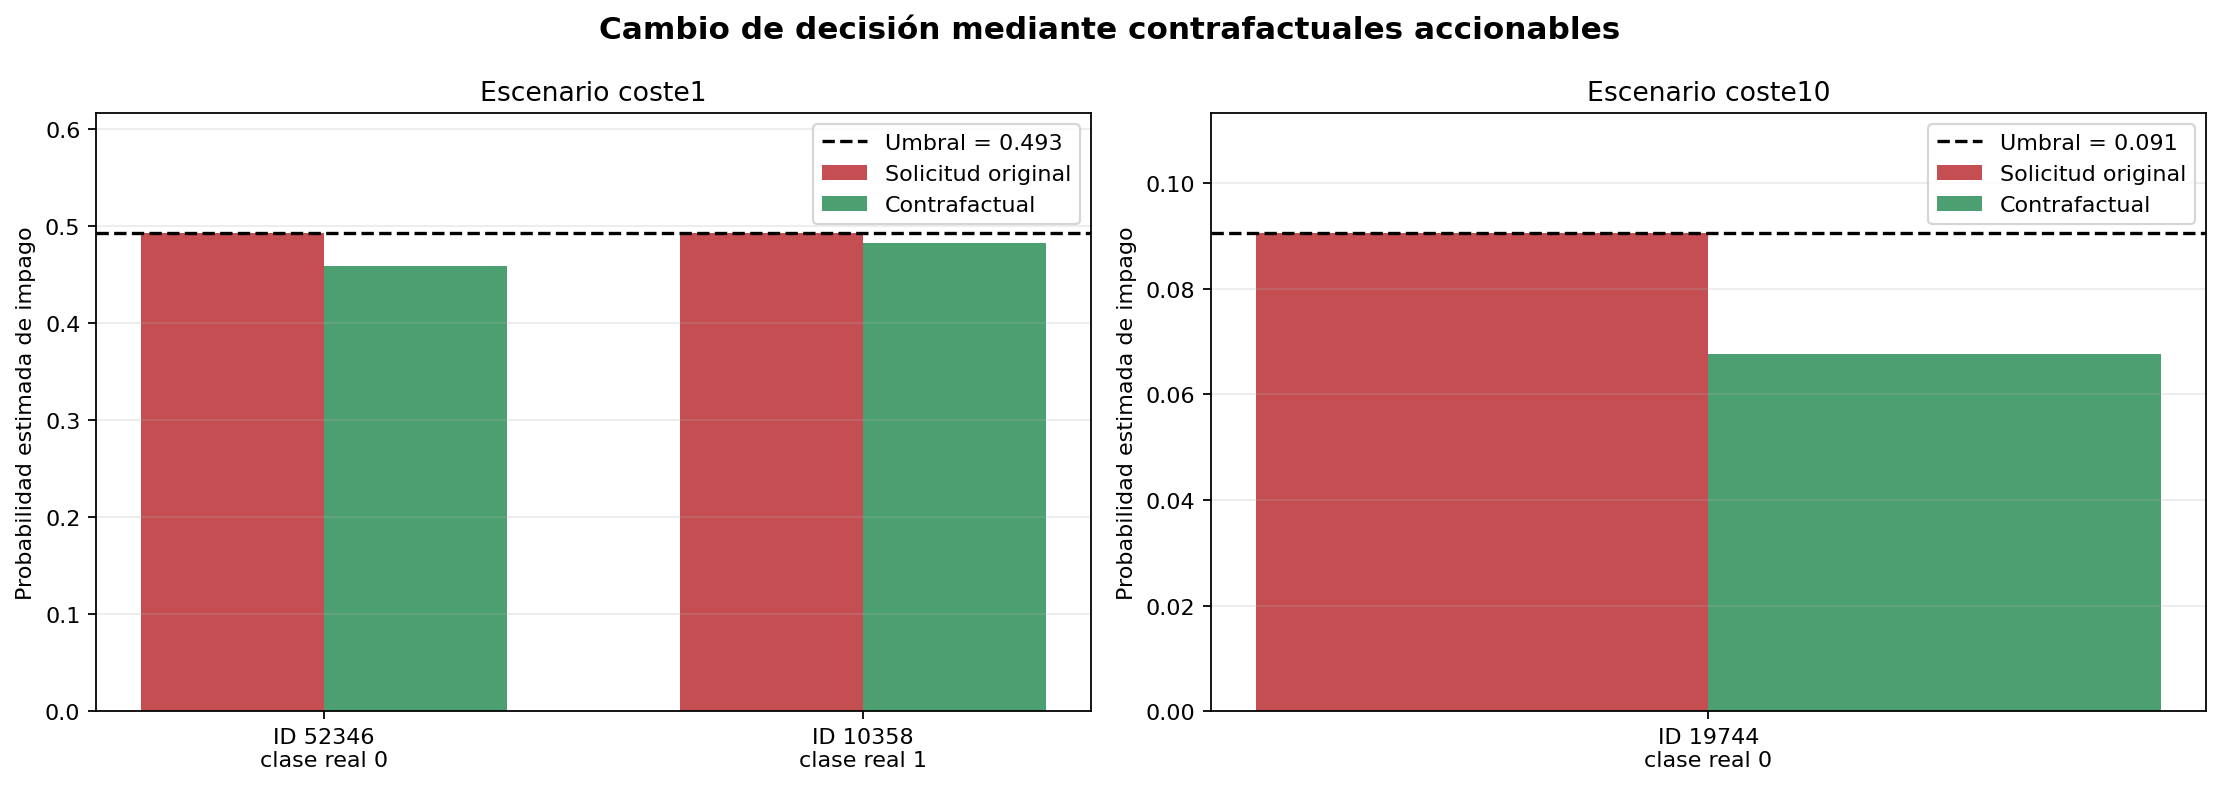
\includegraphics[width=.75\linewidth]{contrafactuals_probabilidad_original_vs_cf.png}
\caption{Probabilidad de impago original frente a probabilidad tras el contrafactual, para los 3 casos con contrafactual generado y plausible (2 puntos en coste1, 1 en coste10). No incluye los 4 casos sin contrafactual ni el caso generado pero descartado por implausible (id\_test=14183).}
\label{fig:cf_probabilidad}
\end{figure}

\subsection{Casos ilustrativos}

\textbf{Caso 52346 (coste1, \texttt{borde\_umbral}, clase\_real=0, falso positivo, contrafactual plausible).} La solicitud fue denegada con un riesgo estimado del $49{,}4\%$, por encima del umbral del escenario ($49{,}3\%$). Reduciendo la utilización de crédito revolving de $110{,}3\%$ a $109{,}3\%$ y aumentando los ingresos mensuales de $4{.}720$ a $5{.}863$ EUR, el riesgo estimado desciende al $45{,}9\%$ y la decisión del modelo se revierte a conceder. Esta es la explicación de referencia para responder a la pregunta \emph{qué decirle a un cliente denegado} cuando existe contrafactual plausible: se comunican los cambios concretos, aclarando siempre que describe el comportamiento del modelo y no constituye una garantía de aprobación futura.

\textbf{Caso 28495 (\texttt{denegacion\_fuerte}, clase\_real=0, sin contrafactual en ningún escenario).} Con $p(\text{impago})=0{,}833$, muy por encima de ambos umbrales, DiCE no encuentra ninguna combinación razonable de cambios en las 4 variables accionables, dentro de los límites establecidos, que revierta la decisión. La respuesta honesta al cliente reconoce que el método no halló una alternativa válida bajo esas restricciones, sin afirmar que la aprobación sea imposible en el futuro.

\textbf{Caso 10358 (coste1, \texttt{borde\_umbral}, clase\_real=1, correctamente denegado).} Riesgo estimado $49{,}4\%$ frente al umbral $49{,}3\%$; subiendo únicamente los ingresos de $2{.}697$ a $3{.}120$ EUR el riesgo baja al $48{,}3\%$ y la decisión se revierte. Al ser \texttt{clase\_real=1}, este contrafactual sirve exclusivamente de auditoría interna del comportamiento del modelo, no como recomendación al cliente.

\textbf{Caso 19744 (coste10, \texttt{borde\_umbral}, clase\_real=0).} Riesgo $9{,}1\%$ frente al umbral $9{,}1\%$ ($\theta=0{,}0906$); bajando la utilización de revolving de $100{,}0\%$ a $70{,}7\%$ el riesgo cae al $6{,}8\%$, ejemplo del escenario asimétrico, más conservador.

\textbf{Caso 14183 (coste10, \texttt{borde\_umbral}, clase\_real=1, contrafactual generado pero descartado).} DiCE encuentra técnicamente una alternativa (\texttt{DebtRatio} de $1{,}283$ a $0{,}908$ y líneas de crédito abiertas de $12$ a $8$, riesgo de $9{,}1\%$ a $6{,}5\%$), pero se descarta en la verificación de plausibilidad: el valor interno del contrafactual para el número de líneas de crédito es fraccionario, no un entero válido (falla la comprobación de conteos enteros). Este caso ilustra un matiz operativo relevante: el texto de cliente ya redondeado ($12\rightarrow 8$) se genera igualmente porque la lógica condiciona el texto a la existencia de un contrafactual generado, no a su plausibilidad; por ello no debería usarse como explicación real pese a tener una redacción aparentemente correcta.

\textbf{Caso 79585 (\texttt{denegacion\_fuerte}, clase\_real=1).} Con $p(\text{impago})=0{,}917$, tampoco se encuentra contrafactual en ninguno de los dos escenarios.

\subsection{Hallazgos}

\begin{itemize}
\item Solo existe contrafactual accionable en los casos \texttt{borde\_umbral} (4/4 generados); en \texttt{denegacion\_fuerte}, 0/4. La distancia al umbral de decisión condiciona por completo si hay una explicación accionable, no la clase real del solicitante.
\item De los 4 contrafactuales generados, 3 son plausibles: $2/2$ en coste1 y $1/2$ en coste10. El único descartado (\texttt{id\_test=14183}, coste10) falla por un conteo no entero en \texttt{NumberOfOpenCreditLinesAndLoans}.
\item Los límites de accionabilidad usados por DiCE son concretos y fijos por diseño: ingresos hasta $+25\%$, revolving y \texttt{DebtRatio} hasta $-30\%$, cierre de hasta dos líneas de crédito; el resto de variables (edad, impagos previos, personas dependientes) permanece fijo.
\item La probabilidad de impago media de los 8 casos seleccionados es $0{,}6843$ en coste1 y $0{,}4829$ en coste10: en ambos escenarios se mezclan casos muy cerca del umbral (\texttt{borde\_umbral}) con otros muy por encima (\texttt{denegacion\_fuerte}), como los casos \texttt{id\_test=28495} y \texttt{id\_test=79585}, repetidos en ambos escenarios con $p(\text{impago})=0{,}833$ y $0{,}917$ respectivamente.
\item La distinción \texttt{uso\_explicacion} (\texttt{explicacion\_cliente\_falso\_positivo} frente a \texttt{auditoria\_interna\_denegacion\_correcta}) marca si el contrafactual se puede comunicar como explicación al cliente o si solo sirve para auditar internamente el modelo: con \texttt{clase\_real=1} (correctamente denegado) nunca debería presentarse como promesa de aprobación, aunque el contrafactual exista y sea plausible.
\item El caso descartado por implausibilidad (\texttt{id\_test=14183}) evidencia un riesgo metodológico general de los sistemas de contrafactuales: la generación de un texto explicativo no garantiza por sí sola su validez; la comprobación de plausibilidad debe aplicarse siempre antes de comunicar cualquier resultado.
\end{itemize}

\section{Auditoría: análisis SHAP global y local (cotejo con LIME)}

Para auditar las decisiones del XGBoost ganador se aplica \textbf{TreeExplainer}, el algoritmo exacto de la librería SHAP (\emph{SHapley Additive exPlanations}) diseñado específicamente para modelos basados en árboles, sobre las 21\,000 observaciones del conjunto de test. El cálculo se repite por separado para el escenario simétrico (\texttt{modelo\_coste1}) y el asimétrico (\texttt{modelo\_coste10}), aunque ambos comparten exactamente el mismo estimador XGBoost y solo difieren en el umbral que traduce la puntuación de riesgo en decisión de conceder o denegar crédito.

\subsection{Metodología: valores de Shapley y aditividad}

El valor de Shapley de la variable $i$ para una instancia $x$, con $N$ el conjunto de las $M$ variables del modelo, se define como el promedio ponderado de su contribución marginal sobre todos los subconjuntos $S$ que no la contienen:

\[
\phi_i(x) = \sum_{S \subseteq N \setminus \{i\}} \frac{|S|!\,(M-|S|-1)!}{M!}\, \Big[ f_x(S \cup \{i\}) - f_x(S) \Big]
\]

TreeExplainer aprovecha la estructura del ensamblado de árboles para calcular estos valores de forma exacta (no aproximada por muestreo), garantizando la propiedad de aditividad local que permite descomponer cualquier predicción individual en la suma de las contribuciones de cada variable:

\[
f(x) = \phi_0 + \sum_{i=1}^{M} \phi_i(x)
\]

donde $\phi_0$ es el valor esperado del modelo sobre el conjunto de referencia (\emph{background}) y $f(x)$ es la salida cruda del XGBoost en escala \emph{log-odds} (margen), no la probabilidad directa: $P(\text{impago}\mid x) = \sigma(f(x)) = 1/(1+e^{-f(x)})$. Esta distinción es relevante para no confundir la magnitud de las barras de un \emph{waterfall} con probabilidades al leerlas junto a los umbrales de decisión (0,4934 en el escenario simétrico, 0,0906 en el asimétrico).

\subsection{Importancia global}

La Figura~\ref{fig:shap_summary_coste1} resume, para el escenario simétrico, la importancia media absoluta de cada variable ($\text{mean\_abs\_shap} = \frac{1}{n}\sum_{j=1}^{n} |\phi_i(x_j)|$ sobre las $n$ observaciones de test) junto con el sentido del efecto (color: rojo = valor alto de la variable, azul = valor bajo).

\begin{figure}[H]
\centering
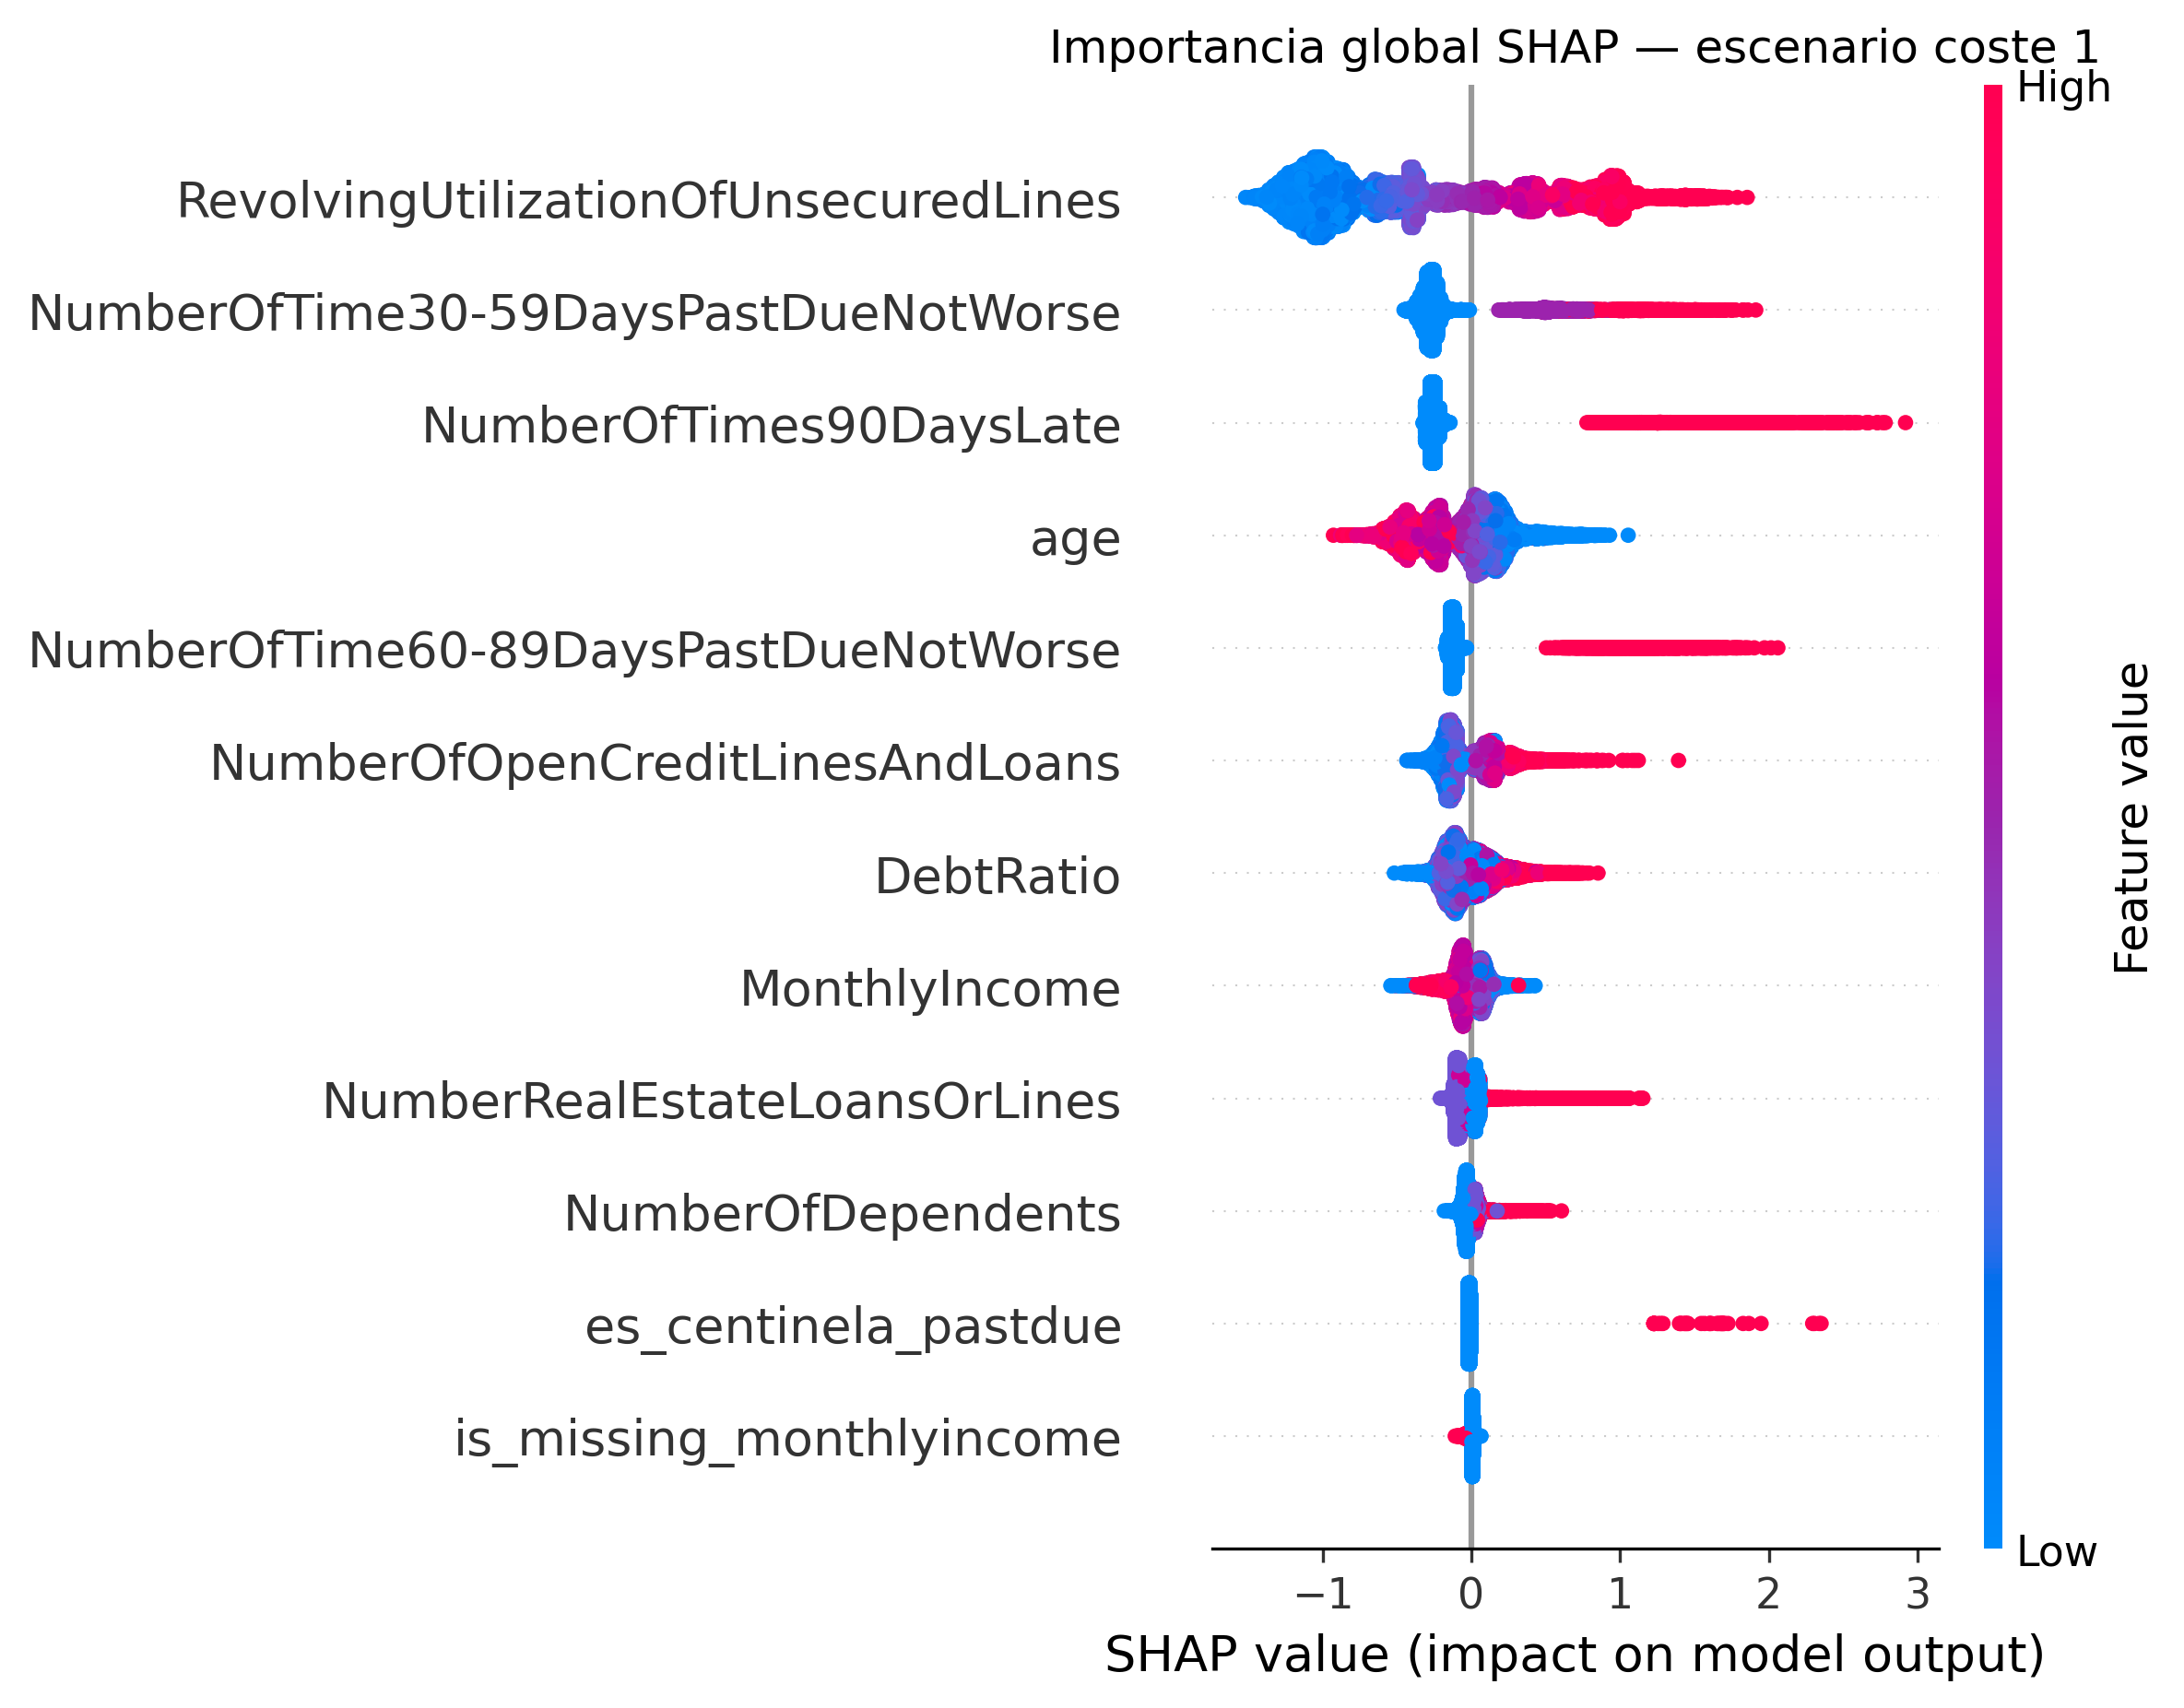
\includegraphics[width=.85\linewidth]{shap_summary_coste1.png}
\caption{Resumen SHAP global, escenario simétrico (coste1): importancia media absoluta por variable y sentido del efecto.}
\label{fig:shap_summary_coste1}
\end{figure}

\texttt{RevolvingUtilizationOfUnsecuredLines} (utilización de crédito revolving) domina la importancia global con $\text{mean\_abs\_shap}=0{,}7873$, más del doble (2,26$\times$) que la siguiente variable, \texttt{NumberOfTime30-59DaysPastDueNotWorse} (0,3486); le siguen \texttt{NumberOfTimes90DaysLate} (0,3278) y \texttt{age} (0,2273). La Tabla~\ref{tab:shap_global} recoge el detalle de las seis variables más importantes.

\begin{table}[H]
\centering
\caption{Importancia global SHAP (\texttt{mean\_abs\_shap}) y ranking, escenario coste1 -- top 6 variables.}
\label{tab:shap_global}
\begin{tabular}{lrr}
\toprule
Variable & mean\_abs\_shap & Ranking \\
\midrule
\texttt{RevolvingUtilizationOfUnsecuredLines} & 0,7873 & 1 \\
\texttt{NumberOfTime30-59DaysPastDueNotWorse} & 0,3486 & 2 \\
\texttt{NumberOfTimes90DaysLate} & 0,3278 & 3 \\
\texttt{age} & 0,2273 & 4 \\
\texttt{NumberOfTime60-89DaysPastDueNotWorse} & 0,1735 & 5 \\
\texttt{NumberOfOpenCreditLinesAndLoans} & 0,1592 & 6 \\
\bottomrule
\end{tabular}
\end{table}

\begin{figure}[H]
\centering
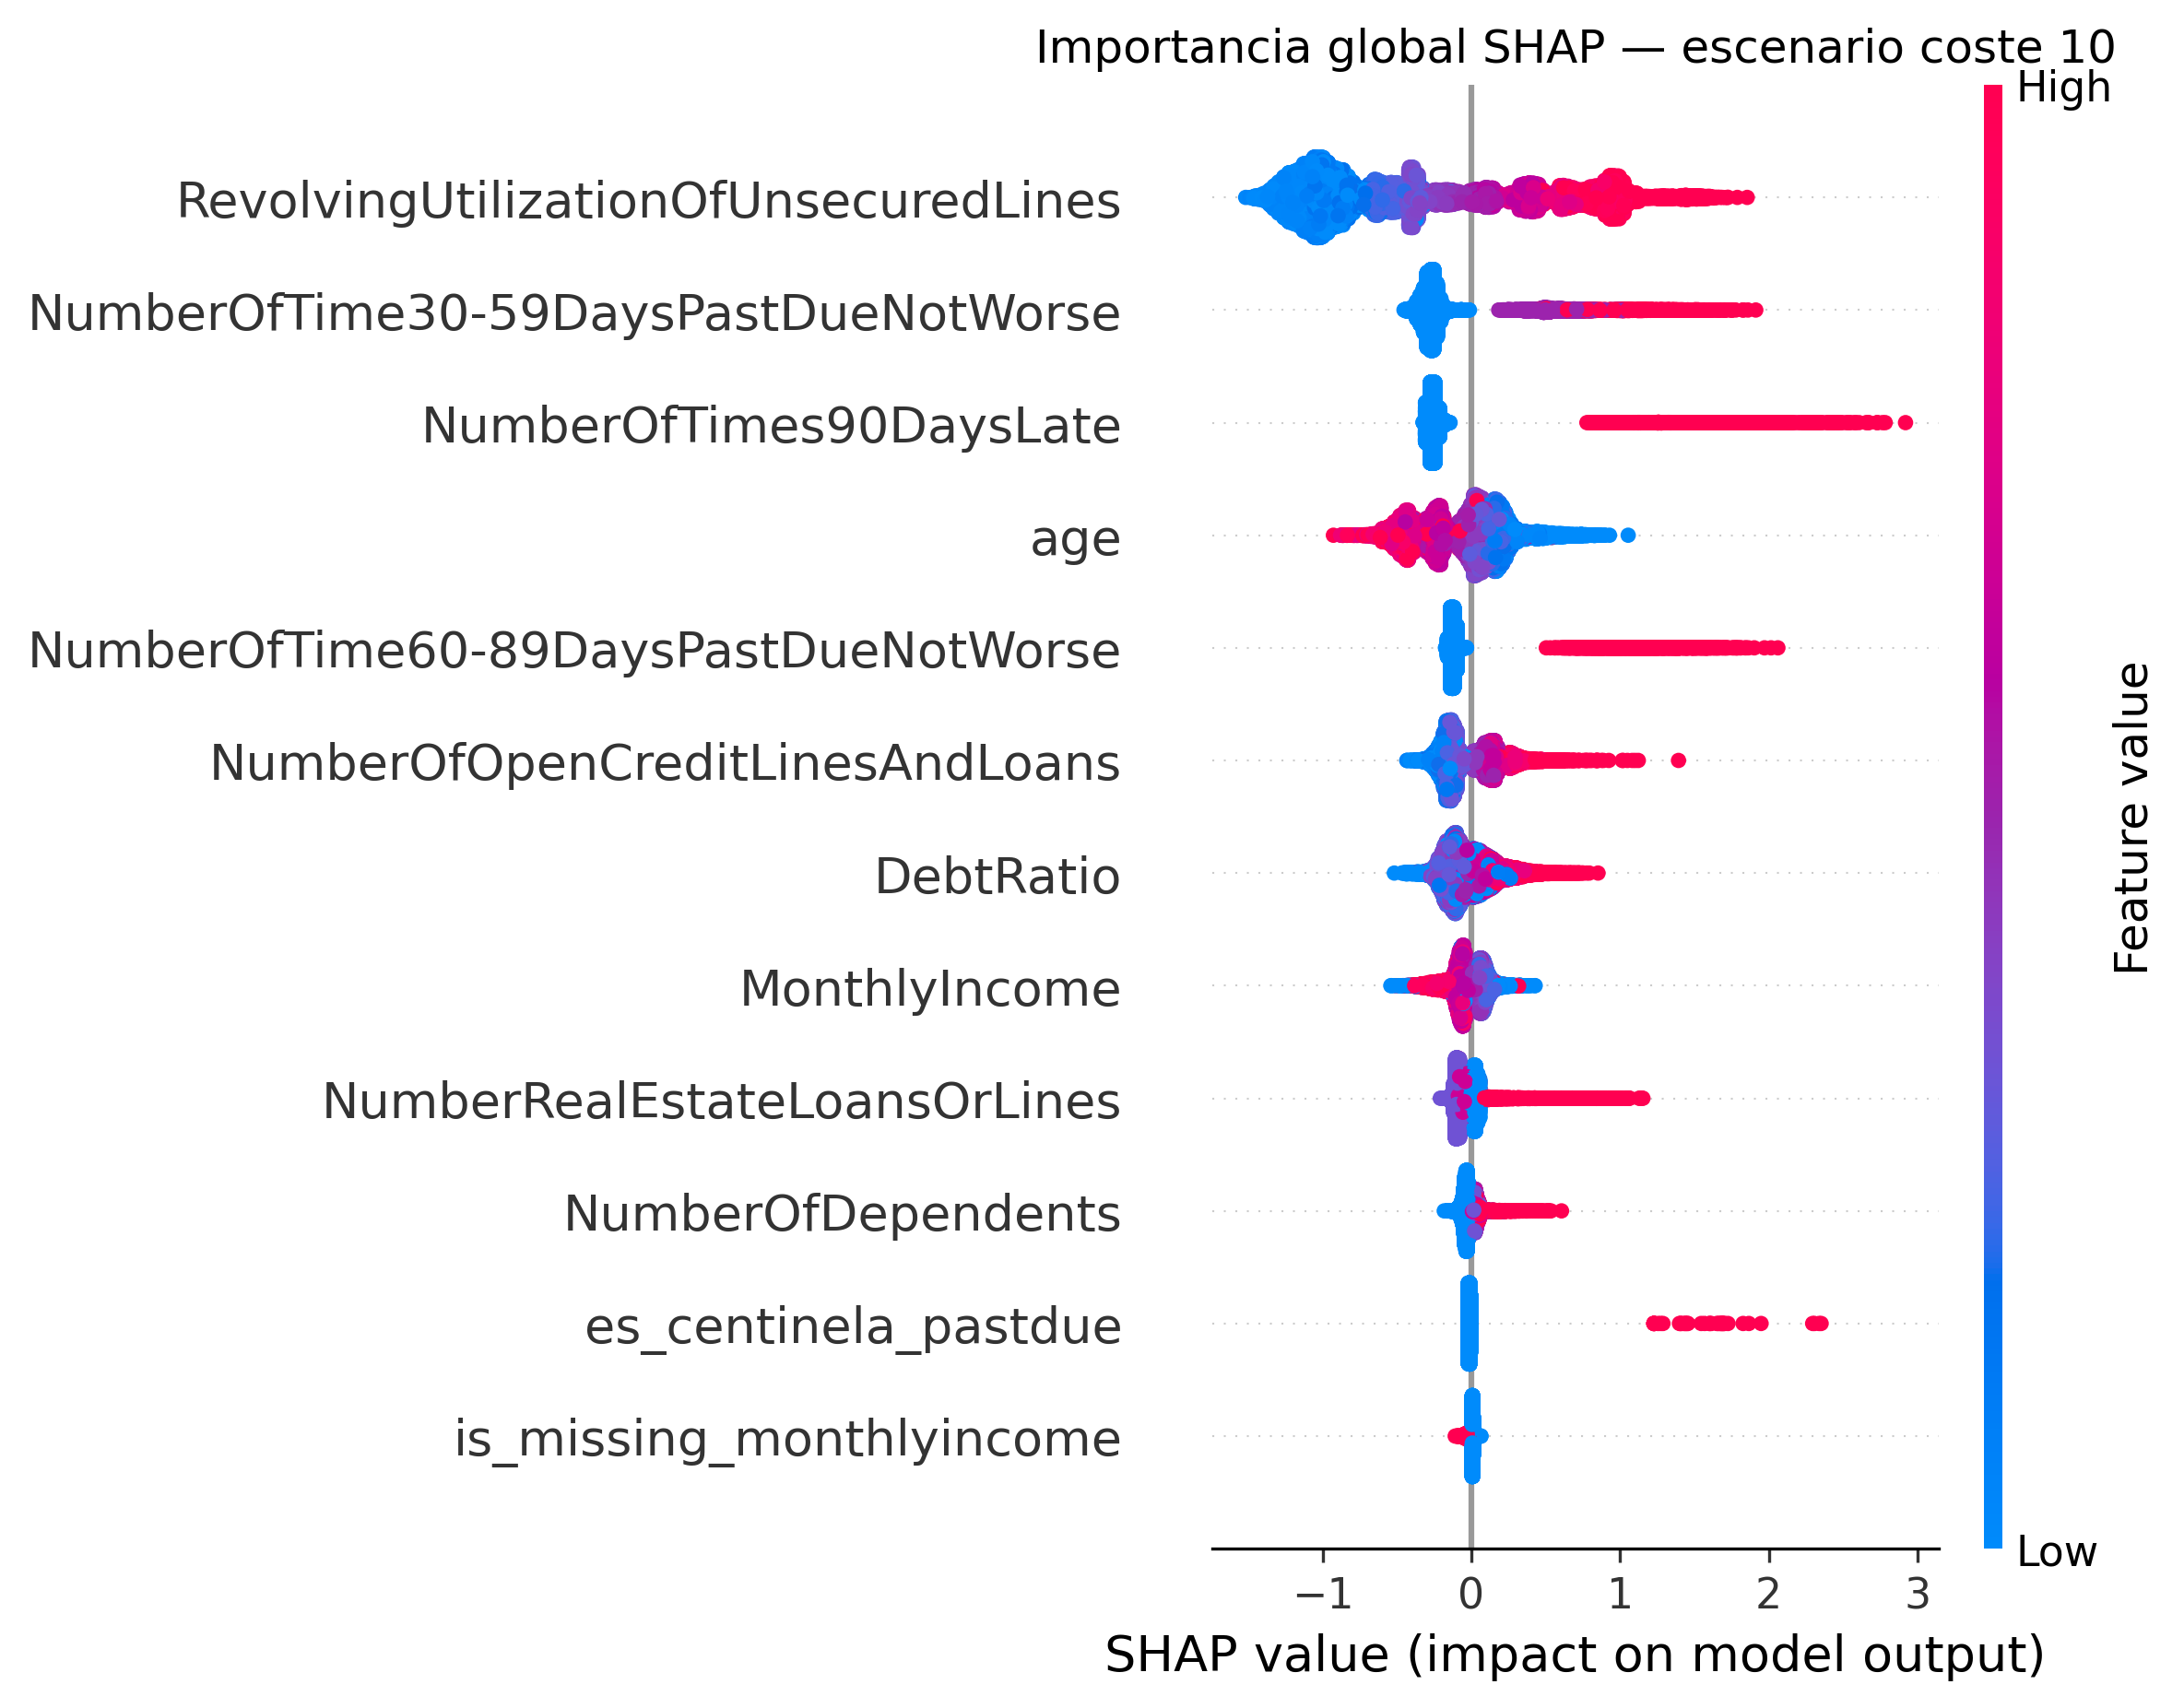
\includegraphics[width=.85\linewidth]{shap_summary_coste10.png}
\caption{Resumen SHAP global, escenario asimétrico (coste10): mismo ranking y mismos valores que en coste1.}
\label{fig:shap_summary_coste10}
\end{figure}

Comparando la Figura~\ref{fig:shap_summary_coste10} con la Figura~\ref{fig:shap_summary_coste1}: son idénticas. Los escenarios coste1 y coste10 comparten exactamente el mismo ranking y los mismos valores SHAP (diferencia máxima $=0$), porque el estimador subyacente es el mismo XGBoost; únicamente cambia el umbral de decisión aguas abajo (0,4934 en coste1 frente a 0,0906 en coste10), elegido según el coste de cada escenario.

\subsection{Explicaciones locales}

Además del resumen global se construyen explicaciones locales tipo \emph{waterfall} para casos individuales denegados, incluido un caso de borde (justo por encima del umbral de decisión). En un \emph{waterfall}, las barras rojas empujan la puntuación hacia el impago y las azules hacia el pago.

\begin{figure}[H]
\centering
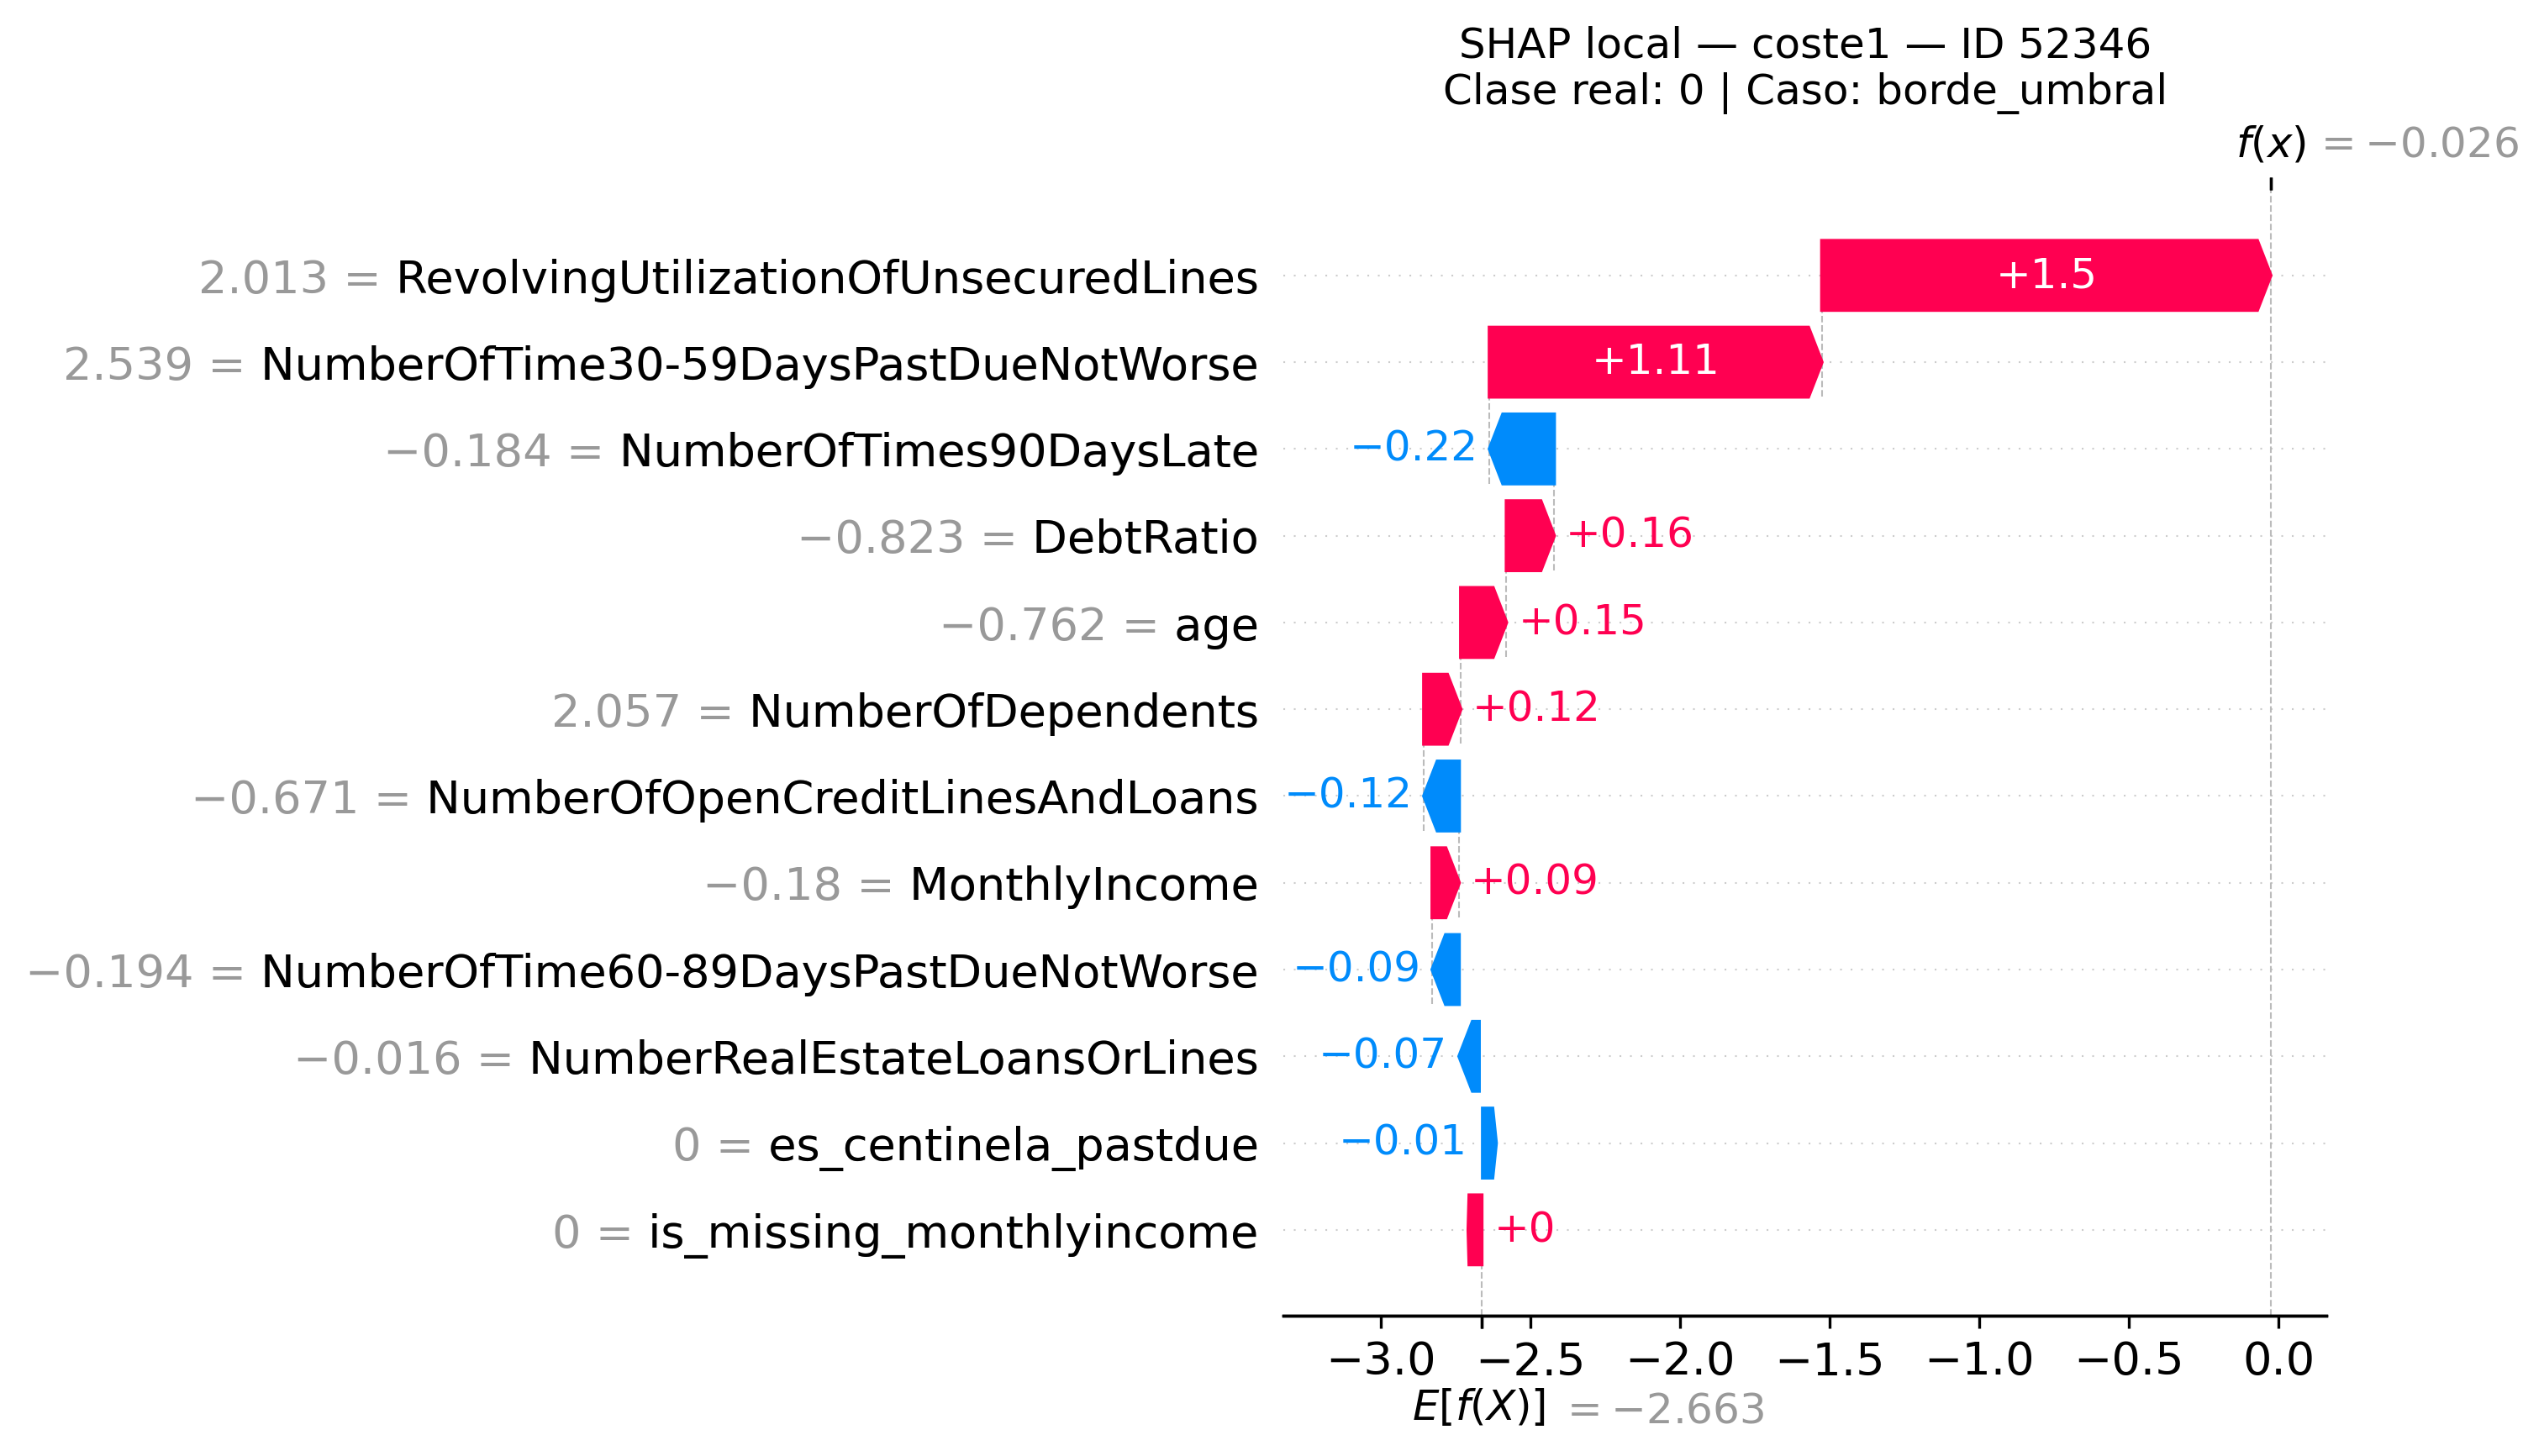
\includegraphics[width=.85\linewidth]{shap_local_coste1_id_52346.png}
\caption{Explicación local SHAP (\emph{waterfall}), caso de borde \texttt{id\_test=52346}, escenario coste1.}
\label{fig:shap_local_52346}
\end{figure}

El caso de borde \texttt{id\_test=52346} (escenario coste1, clase real 0) tiene $P(\text{impago})=0{,}493506$ frente al umbral $\theta=0{,}493394$, un margen de solo $+0{,}000112$: una denegación muy ajustada, prácticamente en el límite exacto de la decisión.

\begin{figure}[H]
\centering
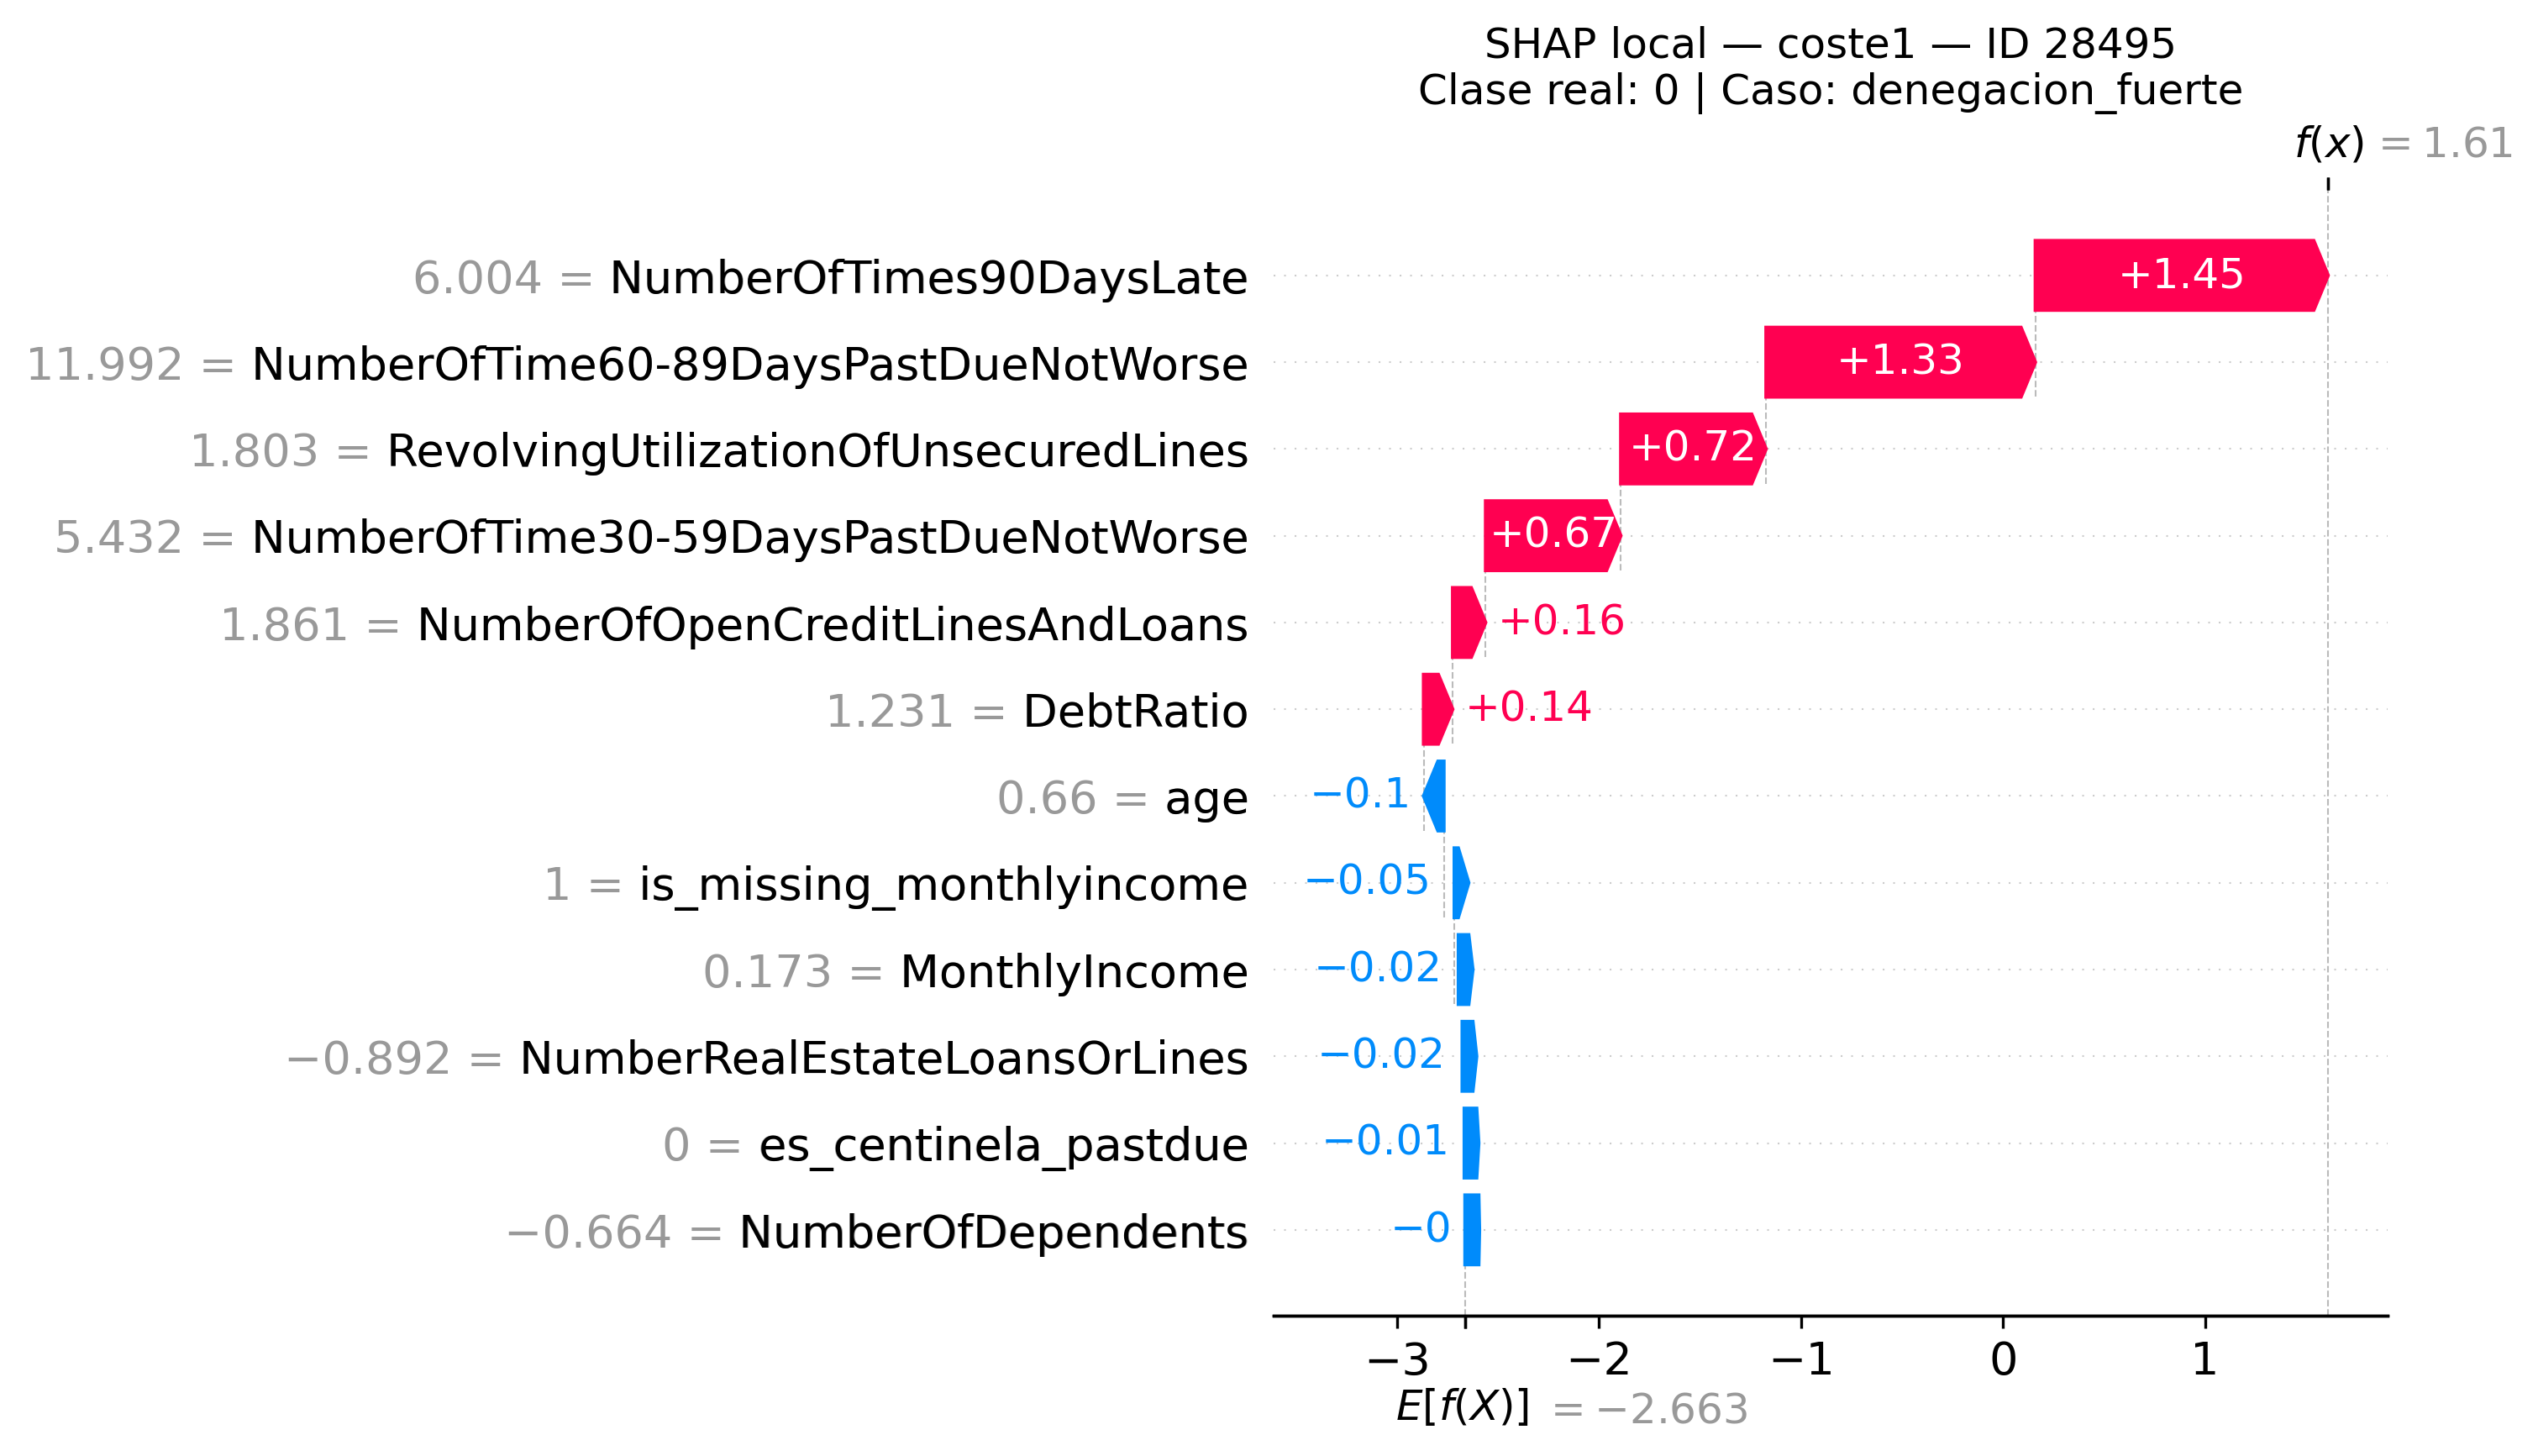
\includegraphics[width=.85\linewidth]{shap_local_coste1_id_28495.png}
\caption{Explicación local SHAP (\emph{waterfall}), caso \texttt{id\_test=28495} (denegación fuerte), escenario coste1.}
\label{fig:shap_local_28495}
\end{figure}

El caso \texttt{id\_test=28495} está presente en ambos escenarios de coste (junto con el \texttt{id\_test=79585}); su explicación SHAP es idéntica en coste1 y coste10 (diferencia máxima $=0{,}0$), evidencia adicional -a nivel de instancia individual- de que el modelo base no cambia entre escenarios y de que toda la diferencia de comportamiento reside en el umbral aplicado.

\subsection{Cotejo de fiabilidad: SHAP frente a LIME}

De forma independiente a las explicaciones anteriores se coteja la fiabilidad de SHAP frente a LIME sobre 6 clientes denegados (3 por escenario, seleccionados aparte de los casos usados en las figuras locales y en la auditoría de contrafactuales): se reejecuta LIME 6 veces por caso para medir cuánto varía el peso que asigna a cada variable, se contrasta con la varianza nula de SHAP -que al ser exacto da siempre el mismo resultado- y se mide el acuerdo entre los rankings de variables de ambos métodos con el coeficiente de correlación de Spearman en valor absoluto:

\[
\rho = 1 - \frac{6 \sum_{k=1}^{n} d_k^2}{n\,(n^2-1)}
\]

donde $d_k$ es la diferencia entre el rango que SHAP y el rango que LIME asignan a la variable $k$, y $n$ es el número de variables comparadas.

\begin{figure}[H]
\centering
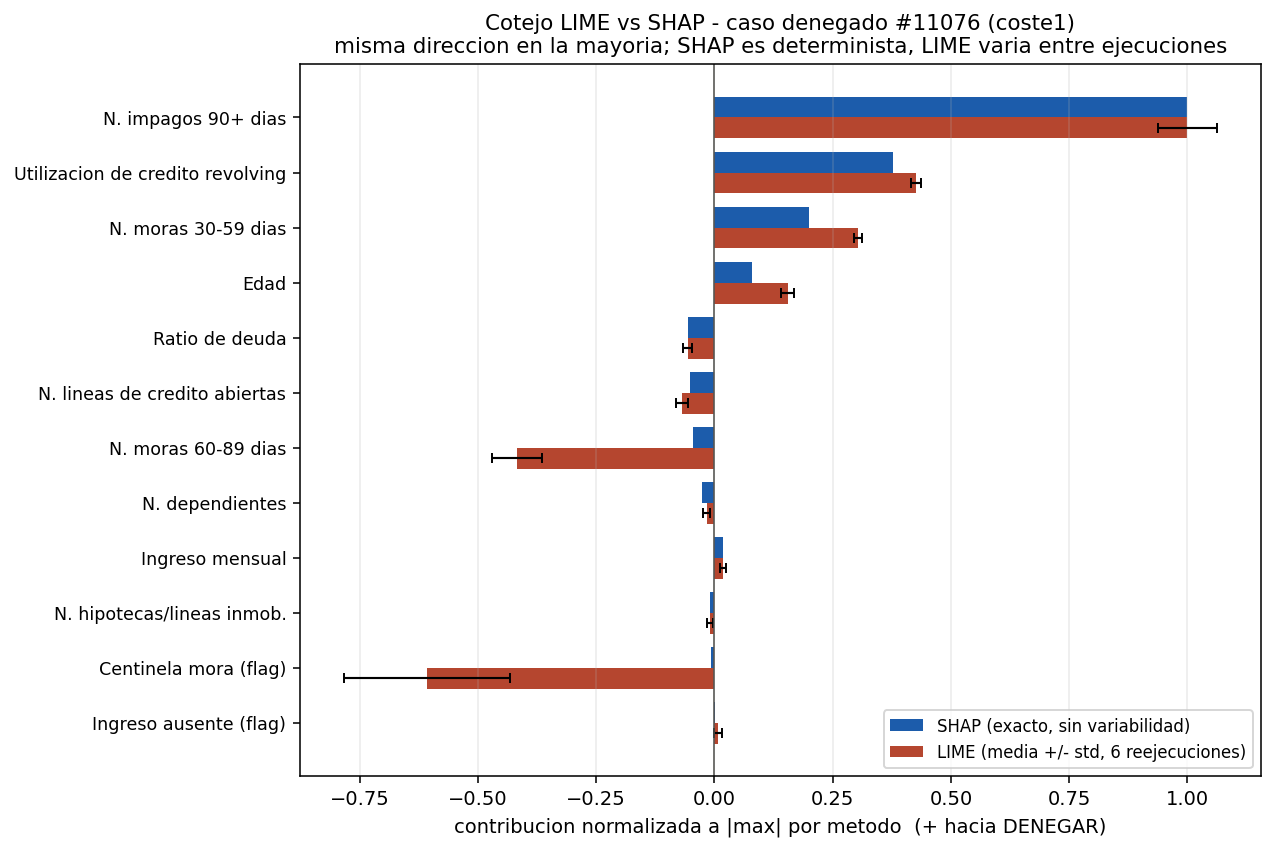
\includegraphics[width=.85\linewidth]{otras_08_lime_vs_shap.png}
\caption{Dispersión de los pesos de LIME entre reejecuciones (barras de error) frente a la ausencia de varianza de SHAP.}
\label{fig:lime_vs_shap}
\end{figure}

\begin{table}[H]
\centering
\caption{Cotejo cuantitativo SHAP vs LIME sobre 6 casos denegados (6 reejecuciones de LIME por caso).}
\label{tab:lime_vs_shap}
\begin{tabular}{lrrrrl}
\toprule
Escenario & idx\_caso & lime\_std\_media & shap\_std & Spearman $|\rho|$ & top1 coincide \\
\midrule
coste1 & 3665 & 0,0057 & 0,0 & 0,5175 & Sí \\
coste1 & 11076 & 0,0055 & 0,0 & 0,6014 & Sí \\
coste1 & 19825 & 0,0056 & 0,0 & 0,3147 & No \\
coste10 & 976 & 0,0057 & 0,0 & 0,5524 & No \\
coste10 & 14834 & 0,0055 & 0,0 & 0,5245 & No \\
coste10 & 17133 & 0,0058 & 0,0 & 0,4266 & No \\
\bottomrule
\end{tabular}
\end{table}

SHAP es exacto y determinista ($\text{shap\_std}=0{,}0$ en los 6 casos evaluados) mientras LIME fluctúa entre reejecuciones ($\text{lime\_std\_media} \approx 0{,}0056$, hasta 0,0357 en el caso coste10 \texttt{idx\_caso=976}); el acuerdo de ranking entre ambos métodos es solo moderado (Spearman medio $\approx 0{,}49$, rango 0,31--0,60) y el top-1 coincide en apenas 2 de los 6 casos. Además, LIME señala \texttt{es\_centinela\_pastdue} (variable centinela de historial de mora) como la variable más inestable en los 6 casos, justo la que SHAP considera casi irrelevante ($\text{mean\_abs\_shap}=0{,}0146$, ranking 11 de 12): SHAP se establece como la referencia más fiable para auditar decisiones individuales.

\subsection*{Hallazgos}

\begin{itemize}
\item \texttt{RevolvingUtilizationOfUnsecuredLines} domina la importancia global con $\text{mean\_abs\_shap}=0{,}7873$, más del doble (2,26$\times$) que la siguiente variable, \texttt{NumberOfTime30-59DaysPastDueNotWorse} (0,3486); le siguen \texttt{NumberOfTimes90DaysLate} (0,3278) y \texttt{age} (0,2273).
\item Los escenarios coste1 y coste10 comparten exactamente el mismo ranking y los mismos valores SHAP (diferencia $=0$) porque es el mismo XGBoost; solo cambia el umbral de decisión (0,4934 frente a 0,0906), confirmado también a nivel de instancia: los \texttt{id\_test} 28495 y 79585 aparecen en ambos escenarios con SHAP idéntico (diferencia máxima $=0{,}0$).
\item SHAP es exacto y determinista ($\text{shap\_std}=0{,}0$ en los 6 casos evaluados) mientras LIME fluctúa entre reejecuciones ($\text{lime\_std\_media}\approx 0{,}0056$, hasta 0,0357 en coste10 \texttt{idx\_caso=976}); el acuerdo de ranking entre ambos métodos es solo moderado (Spearman medio $\approx 0{,}49$, rango 0,31--0,60) y el top-1 coincide en apenas 2 de 6 casos.
\item LIME señala \texttt{es\_centinela\_pastdue} como la variable más inestable en los 6 casos, justo la que SHAP considera casi irrelevante ($\text{mean\_abs\_shap}=0{,}0146$, ranking 11 de 12): SHAP es la referencia más fiable para auditar decisiones individuales.
\item El caso de borde \texttt{id\_test=52346} se decide por un margen mínimo ($+0{,}000112$ sobre el umbral): una denegación tan ajustada refuerza por qué interesa auditar también con contrafactuales, además de con SHAP.
\end{itemize}


\section{Otras técnicas de explicabilidad consideradas}

El enunciado invita a incorporar ``otras técnicas que los estudiantes consideren oportunas''. Se aplican
cuatro técnicas de explicabilidad agnósticas al modelo (operan sobre \texttt{predict\_proba}, sin asumir
estructura de árbol), ejecutadas de forma independiente del árbol subrogado y del análisis SHAP descritos
en apartados anteriores, sobre los dos modelos de coste ya entrenados: el escenario simétrico
($C_{FP}=C_{FN}=1$) y el asimétrico ($C_{FP}=1,\ C_{FN}=10$), que comparten el mismo estimador XGBoost y
solo difieren en el umbral $\theta$ que convierte la puntuación de riesgo en decisión. Las cuatro técnicas
son: (1) importancia por permutación contrastada a tres bandas, (2) dependencia parcial (PDP) y curvas ICE,
incluida una superficie PDP en dos dimensiones, (3) reejecución repetida de LIME para cuantificar su
inestabilidad, y (4) una auditoría descriptiva de subgrupos por tramo de edad.

Limitaciones declaradas de entrada: la importancia por permutación y el PDP/ICE se calculan sobre
submuestras (3000 y 2000 filas respectivamente, no sobre las 21\,000 de test), el PDP en dos dimensiones
usa una rejilla de $15\times 15$ puntos, y LIME solo se reejecuta sobre 3 casos denegados por escenario
(6 en total). Son suficientes para ilustrar el fenómeno, no para generalizar con la misma solidez que el
análisis SHAP completo.

\subsection{Importancia por permutación a tres bandas}

La importancia por permutación mide cuánto empeora el coste esperado de negocio cuando se destruye la
relación entre una variable $x_j$ y el objetivo, barajando aleatoriamente sus valores en la muestra y
manteniendo fijas todas las demás variables y el umbral de decisión $\theta$ vigente en el escenario:

\[
\mathrm{PI}_j(\theta) = C\!\left(\hat{y}^{(\pi_j)}(\theta)\right) - C\!\left(\hat{y}(\theta)\right),
\qquad
C(\theta) = C_{FP}\cdot \mathrm{FP}(\theta) + C_{FN}\cdot \mathrm{FN}(\theta),
\]

donde $\hat{y}^{(\pi_j)}(\theta)$ son las decisiones obtenidas tras permutar $x_j$ y $C(\theta)$ es la misma
función de coste esperado empleada en la selección de umbral de los apartados de modelado. El cálculo se
repite 10 veces sobre una submuestra de 3000 filas de test y se promedia. Este valor se contrasta con dos
referencias adicionales: la importancia nativa de XGBoost (ganancia de impureza acumulada por las
variables en todos los \emph{splits} del árbol, independiente del umbral) y la importancia del árbol
subrogado que imita las decisiones del modelo bajo cada umbral.

\begin{figure}[H]
\centering
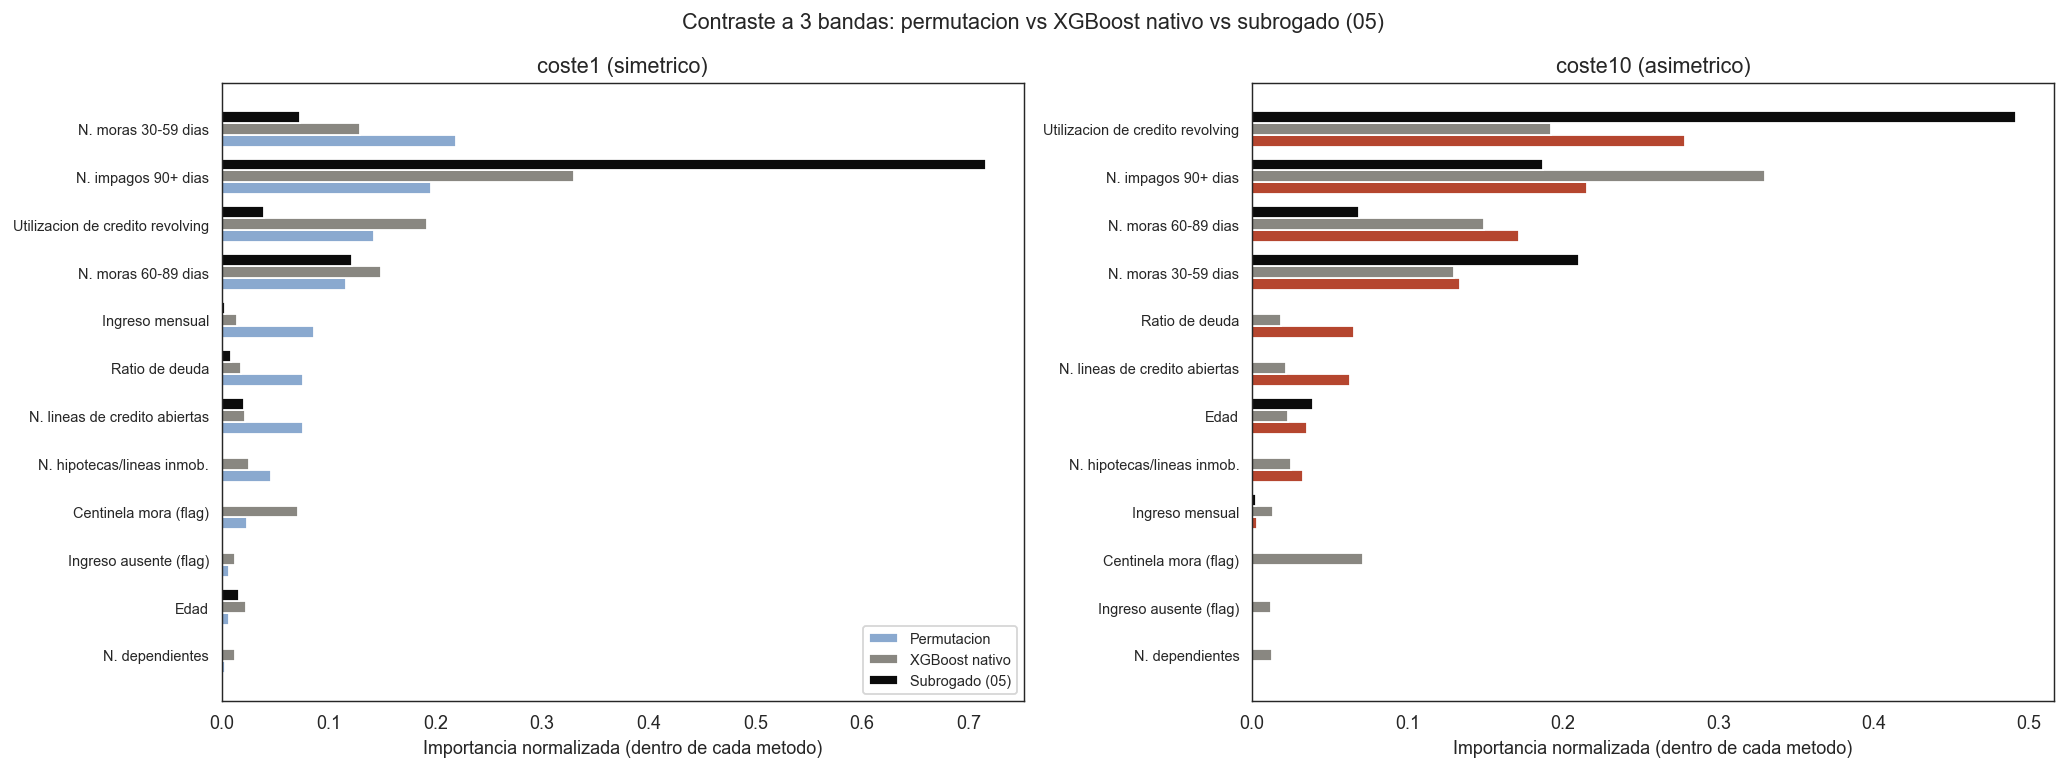
\includegraphics[width=.85\linewidth]{otras_08_permutacion_3bandas.png}
\caption{Importancia a tres bandas (permutación, XGBoost nativo, subrogado) por variable, para el
escenario simétrico (coste1, panel superior) y el asimétrico (coste10, panel inferior).}
\label{fig:permutacion-3bandas}
\end{figure}

\begin{table}[H]
\centering
\caption{Escenario simétrico (coste1): 5 variables principales según XGBoost nativo.}
\begin{tabular}{lrrr}
\toprule
Variable & Permutación (media) & XGBoost nativo & Subrogado (d5) \\
\midrule
N.\ impagos 90+ días & 0.0020 & 0.3301 & 0.7155 \\
Utilización de crédito revolving & 0.0014 & 0.1922 & 0.0397 \\
N.\ moras 60-89 días & 0.0012 & 0.1493 & 0.1219 \\
N.\ moras 30-59 días & 0.0022 & 0.1298 & 0.0734 \\
Centinela mora (flag) & 0.0002 & 0.0715 & N/D \\
\bottomrule
\end{tabular}
\label{tab:permutacion-coste1}
\end{table}

\begin{table}[H]
\centering
\caption{Escenario asimétrico (coste10): 5 variables principales según importancia por permutación.}
\begin{tabular}{lrrr}
\toprule
Variable & Permutación (media) & XGBoost nativo & Subrogado (d5) \\
\midrule
Utilización de crédito revolving & 0.0782 & 0.1922 & 0.4914 \\
N.\ impagos 90+ días & 0.0604 & 0.3301 & 0.1875 \\
N.\ moras 60-89 días & 0.0483 & 0.1493 & 0.0685 \\
N.\ moras 30-59 días & 0.0376 & 0.1298 & 0.2105 \\
Ratio de deuda & 0.0183 & 0.0184 & 0.0000 \\
\bottomrule
\end{tabular}
\label{tab:permutacion-coste10}
\end{table}

\begin{itemize}
\item En coste1 (escenario casi trivial) la importancia por permutación escalada al coste de negocio es
prácticamente plana (0.0000--0.0022): romper cualquier variable apenas mueve un coste esperado que ya es
mínimo, aunque la jerarquía interna de variables se mantenga intacta. En cambio, XGBoost nativo y el
subrogado coinciden con claridad en que \emph{N.\ impagos 90+ días} domina (0.3301 nativo, 0.7155
subrogado).
\item En coste10, permutación y subrogado sí coinciden en que \emph{Utilización de crédito revolving} es
la variable que más pesa en las decisiones actuales (0.0782 permutación, 0.4914 subrogado), pero XGBoost
nativo sigue puntuando más alto \emph{N.\ impagos 90+ días} (0.3301, idéntico a coste1): su importancia
mide ganancia de impureza sobre todos los \emph{splits} del árbol, no está condicionada al umbral vigente
-- una cosa es discriminar mejor en general, otra pesar más en la decisión concreta que se está tomando.
\item Ninguna de las tres métricas cuenta la historia completa por sí sola: la importancia nativa describe
el modelo en abstracto, la del subrogado describe cómo se explican sus decisiones, y la permutación describe
cuánto importa cada variable para el coste de negocio bajo el umbral realmente en uso.
\end{itemize}

\subsection{Dependencia parcial (PDP) y curvas ICE}

El gráfico de dependencia parcial (\emph{Partial Dependence Plot}, PDP) estima el efecto marginal de un
subconjunto de variables $x_S$ sobre la predicción del modelo, promediando sobre la distribución empírica
del resto de variables $x_C$:

\[
\widehat{\mathrm{PDP}}(x_S) = \frac{1}{n}\sum_{i=1}^{n} \hat{f}\!\left(x_S,\, x_C^{(i)}\right),
\]

calculado aquí sobre una submuestra de 2000 filas de test, con $\hat f$ la probabilidad de impago (o de
denegación, una vez aplicado el umbral) predicha por el XGBoost. Las curvas ICE (\emph{Individual
Conditional Expectation}) son las trayectorias individuales $\hat f(x_S, x_C^{(i)})$ sin promediar, una por
observación $i$: permiten detectar heterogeneidad que el PDP, al promediar, podría ocultar. Además del PDP
univariante sobre \emph{Utilización de crédito revolving}, se calcula un PDP en dos dimensiones para la
interacción Edad $\times$ N.\ de moras de 30-59 días, con ambos ejes ya traducidos a años y unidades reales
mediante el pipeline de preprocesado, sobre una rejilla de $15\times 15$ puntos.

\begin{figure}[H]
\centering
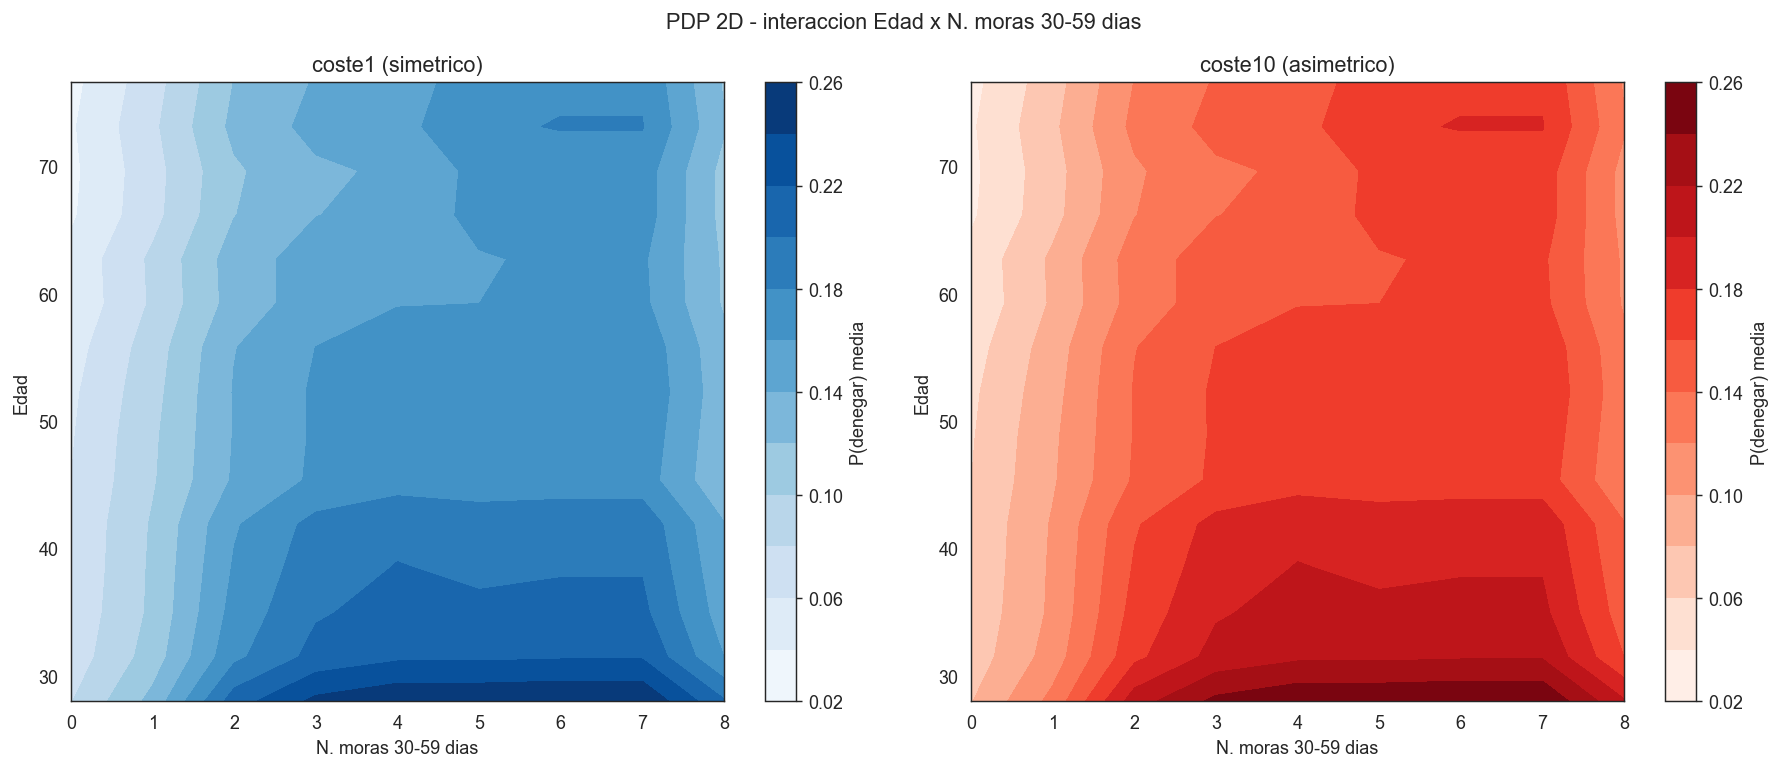
\includegraphics[width=.85\linewidth]{otras_08_pdp2d_interaccion.png}
\caption{PDP en dos dimensiones: interacción Edad $\times$ N.\ de moras de 30-59 días sobre
$P(\text{denegar})$.}
\label{fig:pdp2d}
\end{figure}

\begin{figure}[H]
\centering
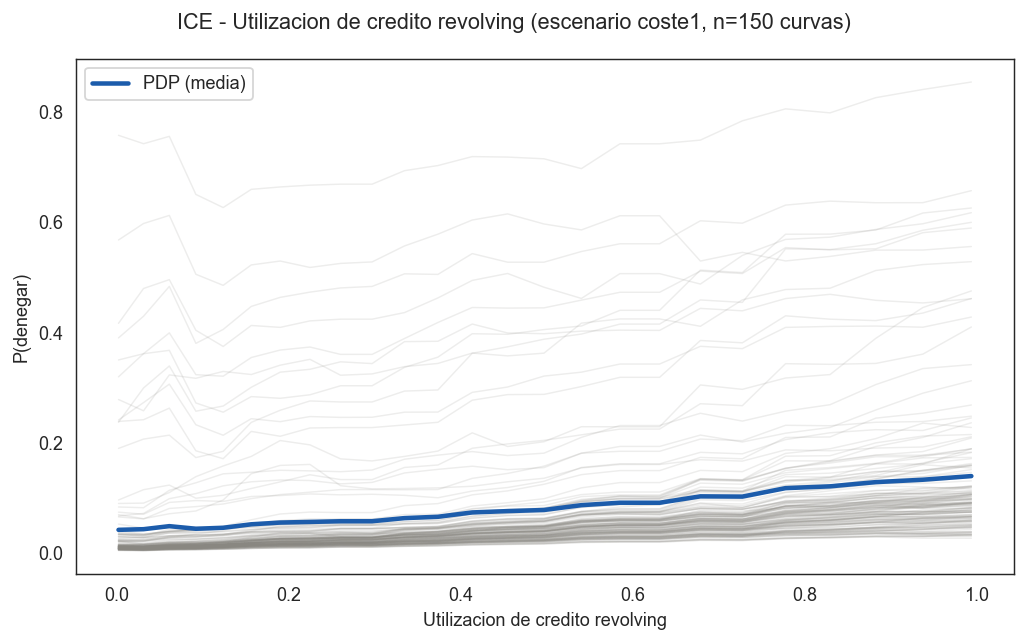
\includegraphics[width=.85\linewidth]{otras_08_ice_revolving.png}
\caption{Curvas ICE individuales y PDP (línea gruesa) de \emph{Utilización de crédito revolving}.}
\label{fig:ice-revolving}
\end{figure}

\begin{itemize}
\item El rango de $P(\text{denegar})$ explicado solo por la edad es 0.0448 sin historial de mora frente a
0.0888 con 8 moras (el máximo de la rejilla) -- prácticamente el doble --, lo que confirma con un método
agnóstico independiente del árbol subrogado la interacción Edad $\times$ mora que ya aparecía dentro de las
reglas del subrogado.
\item Matiz relevante: la superficie de probabilidad del PDP es idéntica entre los dos escenarios de coste,
porque es el mismo estimador XGBoost; lo único que cambia entre coste1 y coste10 es dónde corta cada umbral
esa misma geometría. Esto refina, no contradice, la idea de ``dos personalidades de riesgo'': la
personalidad distinta está en el umbral, no en el modelo.
\item La mayoría de las curvas ICE de \emph{Utilización de crédito revolving} sube de forma monótona, pero
el punto en el que empiezan a subir difiere bastante entre clientes: la variable que domina la importancia
en las decisiones del escenario asimétrico no actúa igual para todos los perfiles de riesgo, información que
el PDP promedio por sí solo no muestra.
\end{itemize}

\subsection{Estabilidad de LIME}

LIME (\emph{Local Interpretable Model-agnostic Explanations}) ajusta, para una instancia $x$, un modelo
sustituto local $g$ interpretable (lineal) que aproxima el comportamiento del modelo $f$ en un entorno de
$x$ definido por una distribución de perturbaciones ponderada por proximidad $\pi_x$:

\[
\xi(x) = \operatorname*{arg\,min}_{g \in G} \; \mathcal{L}(f, g, \pi_x) + \Omega(g),
\]

con $\Omega(g)$ una penalización de complejidad. Al depender de un muestreo aleatorio de perturbaciones, dos
ejecuciones de LIME sobre la misma instancia $x$ pueden producir coeficientes $g$ distintos. Se reejecuta
LIME 6 veces sobre los mismos 3 casos denegados por escenario (6 casos en total) y se mide, para cada
combinación caso-variable, la desviación típica del peso asignado (\texttt{peso\_std}) entre las 6
repeticiones, usando los índices internos de LIME en lugar de parsear el texto de sus explicaciones.

\begin{figure}[H]
\centering
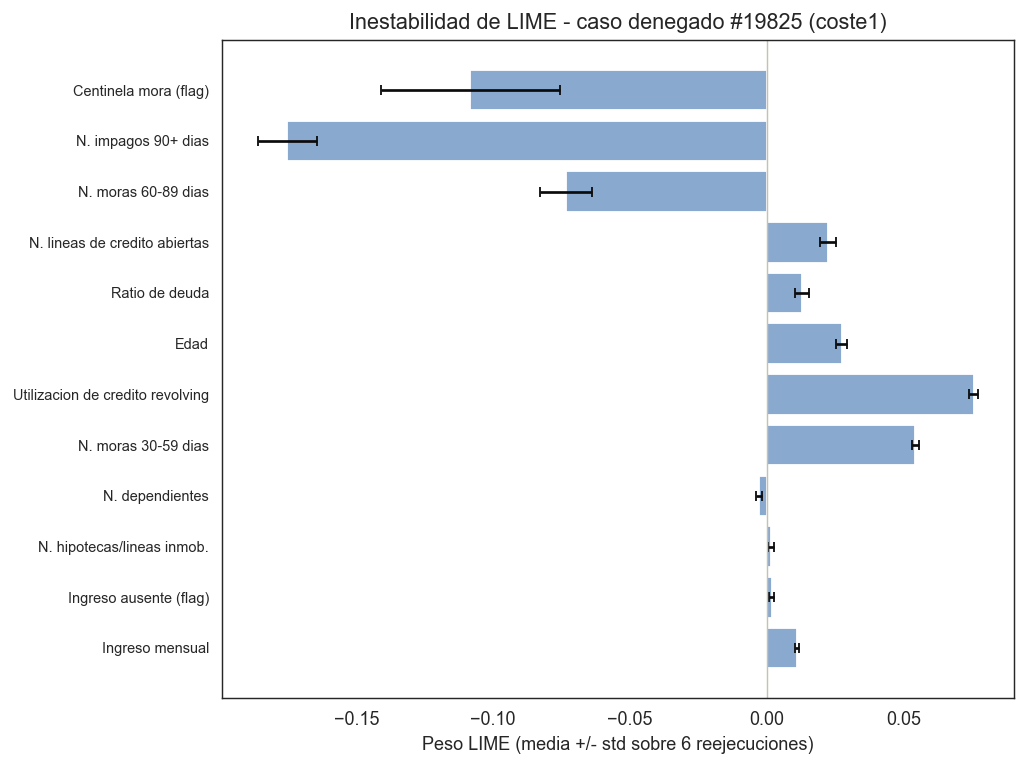
\includegraphics[width=.85\linewidth]{otras_08_lime_inestabilidad.png}
\caption{Dispersión (barras de error) del peso asignado por LIME a cada variable, en 6 reejecuciones sobre
el mismo caso.}
\label{fig:lime-inestabilidad}
\end{figure}

\begin{itemize}
\item \texttt{es\_centinela\_pastdue} (variable centinela de historial de mora) es, con diferencia, la
variable más inestable: \texttt{peso\_std} medio de 0.0322 (máximo 0.0357), aproximadamente el triple que la
siguiente variable en el ranking de inestabilidad, \emph{N.\ impagos 90+ días} (\texttt{std} = 0.0106).
\item En 9 de las 72 combinaciones caso-variable evaluadas (6 casos $\times$ 12 variables) el peso cambia de
signo entre reejecuciones, siempre concentrado en variables de relleno del ranking (Ingreso ausente, Ratio
de deuda, N.\ de hipotecas/líneas inmobiliarias) y nunca en las de mayor peso (impagos, utilización de
crédito), que mantienen el signo estable en las 6 repeticiones.
\item Esta inestabilidad, confirmada aquí de forma autónoma (el cotejo cuantitativo frente a SHAP se detalla
en la sección anterior), refuerza la preferencia por SHAP como técnica principal de auditoría local, al ser
determinista frente a un método muestreado.
\end{itemize}

\subsection{Auditoría descriptiva de subgrupos por tramo de edad}

El Reglamento europeo de Inteligencia Artificial clasifica los sistemas de \emph{scoring} crediticio como
sistemas de ``alto riesgo'', lo que motiva revisar si la tasa de denegación se aleja de la tasa de impago
real dentro de subgrupos poblacionales. El conjunto de datos no incluye ningún atributo protegido explícito;
la edad es el proxy más cercano disponible, de modo que este análisis es una auditoría descriptiva sobre los
6 tramos decadales ya usados en el preprocesado ($\leq 30$, 31-40, 41-50, 51-60, 61-70, $>70$ años), no un
análisis de equidad formal: no se calculan métricas estándar de \emph{fairness} como \emph{equalized odds}.

\begin{figure}[H]
\centering
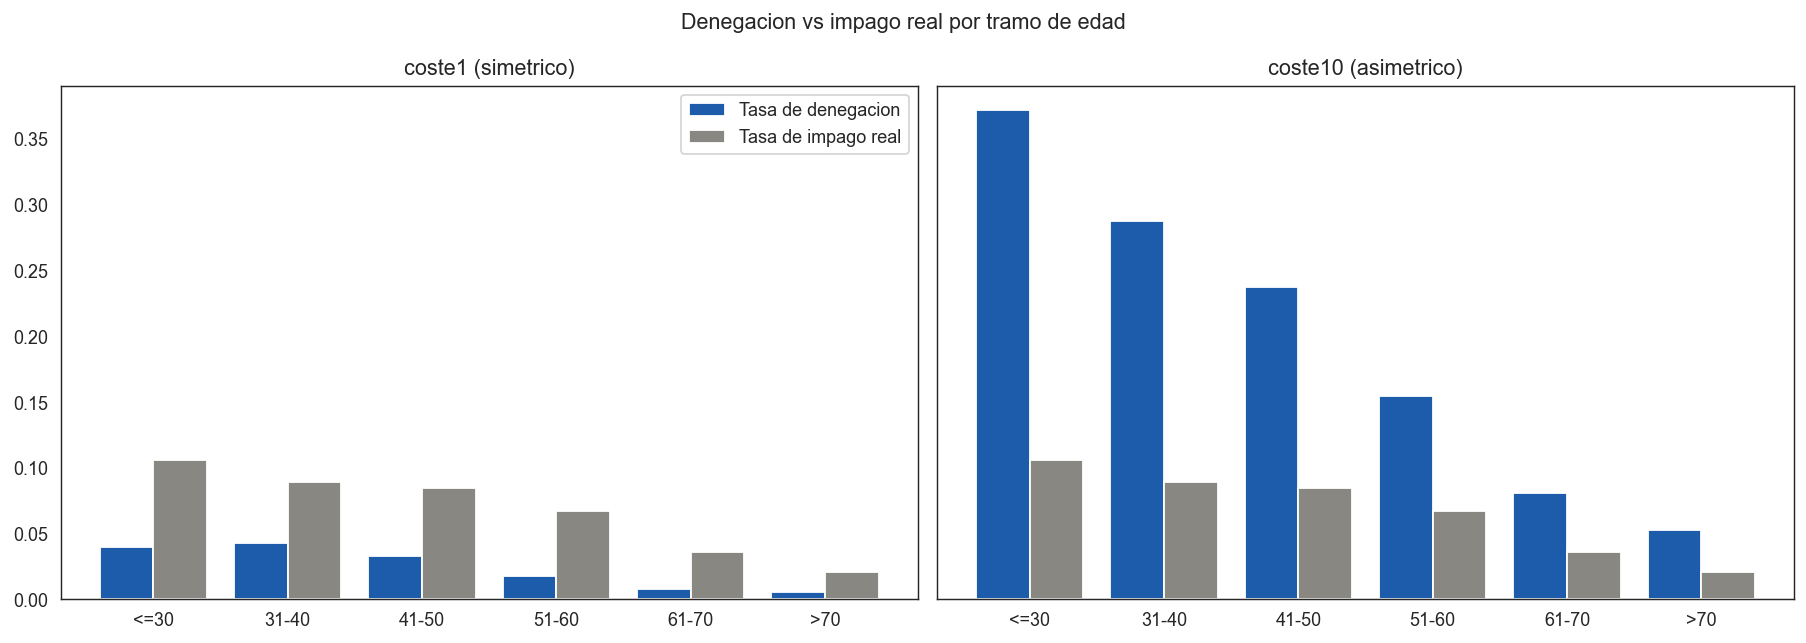
\includegraphics[width=.85\linewidth]{otras_08_subgrupos_edad.png}
\caption{Tasa de denegación frente a tasa de impago real por tramo de edad, escenario simétrico (coste1)
y asimétrico (coste10).}
\label{fig:subgrupos-edad}
\end{figure}

\begin{table}[H]
\centering
\small
\caption{Tasa de denegación, tasa de impago real y coste medio por tramo de edad y escenario (test,
$n=21\,000$).}
\begin{tabular}{llrrrr}
\toprule
Escenario & Tramo de edad & $n$ & Tasa denegación & Tasa impago real & Coste medio \\
\midrule
coste1 & $\leq 30$ & 1562 & 0.0397 & 0.1056 & 0.1005 \\
coste1 & 31-40 & 3431 & 0.0426 & 0.0895 & 0.0871 \\
coste1 & 41-50 & 4951 & 0.0329 & 0.0844 & 0.0774 \\
coste1 & 51-60 & 4896 & 0.0178 & 0.0674 & 0.0639 \\
coste1 & 61-70 & 3734 & 0.0075 & 0.0356 & 0.0351 \\
coste1 & $>70$ & 2426 & 0.0054 & 0.0210 & 0.0198 \\
coste10 & $\leq 30$ & 1562 & 0.3720 & 0.1056 & 0.4424 \\
coste10 & 31-40 & 3431 & 0.2874 & 0.0895 & 0.4223 \\
coste10 & 41-50 & 4951 & 0.2371 & 0.0844 & 0.3882 \\
coste10 & 51-60 & 4896 & 0.1544 & 0.0674 & 0.3409 \\
coste10 & 61-70 & 3734 & 0.0809 & 0.0356 & 0.2132 \\
coste10 & $>70$ & 2426 & 0.0523 & 0.0210 & 0.1447 \\
\bottomrule
\end{tabular}
\label{tab:subgrupos-edad}
\end{table}

\begin{itemize}
\item La denegación sigue la \textbf{dirección} del riesgo real (decrece con la edad) pero no su
\textbf{magnitud}, sobre todo en los más jóvenes. Bajo el escenario asimétrico, el cociente
tasa\_denegación / tasa\_impago\_real es 3.52 en el tramo $\leq 30$ años, desciende hasta un mínimo de 2.27
en 61-70 años y repunta a 2.49 en $>70$: entre 2.3 y 2.5 en los tramos de mayor edad, nunca tan bajo como el
mínimo sugeriría a primera vista.
\item Bajo el escenario simétrico el mismo patrón es mucho más débil y no monótono (cocientes entre 0.21 y
0.48), coherente con que ese escenario es casi trivial (apenas mejora sobre conceder a todos) y su señal de
subgrupo es más ruidosa.
\item \textbf{Lectura honesta:} este patrón no demuestra discriminación causal. La edad puede actuar como
variable proxy de factores no observados en el conjunto de datos (antigüedad crediticia, estabilidad
laboral), y la señal es precisamente más fuerte en el escenario donde el modelo aporta más valor de negocio
real (coste10). Se trata de una mini-auditoría de sesgo descriptiva, no de un análisis de equidad formal.
\end{itemize}

\subsection{Síntesis de las cuatro técnicas}

\begin{itemize}
\item La importancia a tres bandas (permutación, XGBoost nativo, subrogado) no cuenta la misma historia en
los dos escenarios: en coste1 la permutación queda casi plana (0.0000--0.0022) mientras nativo y subrogado
coinciden en \emph{N.\ impagos 90+ días}; en coste10 permutación y subrogado coinciden en \emph{Utilización
de crédito revolving}, pero la importancia nativa de XGBoost no cambia entre escenarios porque no depende
del umbral.
\item El PDP en dos dimensiones confirma, con un método agnóstico independiente del subrogado, que el
efecto de la edad sobre $P(\text{denegar})$ es aproximadamente el doble en presencia de historial de mora
(0.0448 frente a 0.0888); la superficie de probabilidad es idéntica en ambos escenarios de coste, solo
cambia dónde corta el umbral.
\item LIME reejecutado 6 veces sobre el mismo caso produce pesos distintos, con \texttt{es\_centinela\_pastdue}
como variable más inestable (\texttt{peso\_std} medio 0.0322, hasta 3 veces la siguiente) y 9 de 72 cambios
de signo, siempre en variables de relleno del ranking: confirma empíricamente la conveniencia de usar SHAP
(determinista) como referencia principal de auditoría local.
\item Los subgrupos por tramo de edad siguen la dirección del riesgo real pero no su magnitud, con un efecto
mucho más marcado bajo coste asimétrico (cocientes 2.27--3.52) que bajo coste simétrico (0.21--0.48); es una
auditoría descriptiva, no causal ni de equidad formal, dadas las limitaciones de muestreo declaradas al
inicio de esta sección (2000--3000 filas para permutación y PDP/ICE, rejilla $15\times 15$ para el PDP 2D, 3
casos por escenario para LIME).
\end{itemize}

\section{Decisiones de diseño}

Esta sección sistematiza, con criterio metodológico, las decisiones técnicas más relevantes del
proyecto. Cada una se documentó comparando alternativas concretas frente a la evidencia numérica
que las decidió, evitando así que una elección quede justificada solo por intuición. Se agrupan en
ocho bloques: paradigma de modelado, arquitectura de umbrales, familia de modelo, preprocesado
(imputación, tratamiento de outliers y de duplicados), protocolo de validación anti-fuga, definición
del coste del escenario asimétrico, complejidad del árbol subrogado y diseño de la auditoría de
explicabilidad (contrafactuales, SHAP local y técnicas adicionales del bloque de otras técnicas).

\subsection{Metodología de documentación}

Se consideran ``decisiones cerradas'' aquellas que (i) enfrentan al menos dos alternativas
explícitas, (ii) se resuelven con una métrica cuantitativa comparable entre ellas y (iii) tienen
impacto directo sobre el coste de negocio o sobre la fiabilidad de la auditoría. Bajo este criterio
se documentan las 15 decisiones más importantes del proyecto, resumidas en las
Tablas~\ref{tab:decisiones-1} y~\ref{tab:decisiones-2}. El identificador (\texttt{ID}) es una
referencia secundaria de trazabilidad interna; cada fila se explica por sí sola junto con la
evidencia numérica que la respalda.

\subsection{Resumen de las decisiones cerradas}

\begin{table}[H]
\centering
\footnotesize
\caption{Decisiones de diseño (I): paradigma de modelado, preprocesado y protocolo de validación.}
\label{tab:decisiones-1}
\begin{tabular}{p{1.6cm}p{4.4cm}p{7.5cm}}
\toprule
ID & Decisión & Elección final (evidencia) \\
\midrule
D-0.1 & Supervisado vs.\ bandit contextual multibrazo & Supervisado XGBoost: coste de test en el
escenario asimétrico $=0.3275$ frente a $\sim 0.359$ del LinUCB por validación cruzada \\
D-0.2 & Un modelo con dos umbrales vs.\ un modelo por escenario & Un único XGBoost re-umbralizado
dos veces: las probabilidades \emph{out-of-fold} (OOF) coinciden byte a byte entre escenarios
($\max|\Delta|=0$) \\
D-0.3 & Familia de modelo (lineal, red neuronal, árboles, bandit) & XGBoost gana en ambos
escenarios; brecha frente a la regresión logística de $0.033$ en el escenario asimétrico y de
$0.0006$ en el simétrico \\
D-1.1 & Imputación de nulos (\texttt{MonthlyIncome}, \texttt{NumberOfDependents}) & Mediana
condicionada al tramo de edad más indicador de ausencia (\emph{missing not at random}) para el
ingreso; moda (valor $0$) sin indicador para el número de dependientes \\
D-1.2 & Outliers y cola anómala de \texttt{DebtRatio} & Recalcular la variable tras imputar el
ingreso, en vez de winsorizar la cola a ciegas: el estadístico de Kolmogorov--Smirnov entre la cola
y la distribución sana baja de $0.9284$ a $0.1671$ (detalle en la Tabla~\ref{tab:debtratio}) \\
D-1.4 & División train / test & Partición estratificada 80/20 ($84\,000$ / $21\,000$ filas)
realizada \emph{antes} de estimar cualquier parámetro, para evitar fuga de información \\
D-1.6 & Filas duplicadas & Se conservan ($331$ en train, $101$ en producción): sin un identificador
único no puede probarse que sean un error de captura \\
D-2.1 & Protocolo de validación (umbral y familia ganadora) & Validación cruzada de 5 particiones
sobre probabilidades OOF de train; el conjunto de test se reserva íntegramente para el reporte
final \\
\bottomrule
\end{tabular}
\end{table}

\begin{table}[H]
\centering
\footnotesize
\caption{Decisiones de diseño (II): coste del escenario asimétrico, subrogado y auditoría XAI.}
\label{tab:decisiones-2}
\begin{tabular}{p{1.6cm}p{4.4cm}p{7.5cm}}
\toprule
ID & Decisión & Elección final (evidencia) \\
\midrule
D-3.1 & Umbral analítico vs.\ umbral empírico & Se opera con el umbral empírico: $0.4934$ en el
escenario simétrico (analítico $0.5000$) y $0.0906$ en el asimétrico (analítico $1/11=0.0909$) \\
D-3.2 & Coste del escenario 2 & Asimétrico, con $C_{FN}=10 \times C_{FP}$ (errata del enunciado
confirmada por el profesor); el cambio de umbral provoca $7279$ cambios de decisión sobre el
conjunto de producción \\
D-5.1 & Complejidad del árbol subrogado & Dos árboles fijados por escenario: uno
\texttt{operativo} (\texttt{max\_depth=5}, 23 hojas) que maximiza la fidelidad y uno de
\texttt{bolsillo} (\texttt{max\_depth=3}, 8 hojas) legible para el cliente \\
D-6.1 & Herramienta de contrafactuales & DiCE con método aleatorio (\emph{random}), acoplado a un
adaptador que traslada la frontera interna de decisión de DiCE al umbral de negocio real de cada
escenario \\
D-6.2 & Número de casos contrafactuales auditados & 8 casos (2 por clase real $\times$ 2
escenarios): 2 contrafactuales plausibles en el escenario simétrico y 1 en el asimétrico \\
D-7.1 & Instancias y explicador para SHAP local & Los mismos 8 casos que en la fila anterior,
explicados con \texttt{TreeExplainer}, el método exacto y determinista para modelos de árboles \\
D-8.1 & Técnicas de explicabilidad adicionales (bloque de otras técnicas) & Importancia por
permutación, PDP/ICE (incluida interacción 2D), reejecuciones de LIME y auditoría descriptiva por
subgrupos de tramo de edad \\
\bottomrule
\end{tabular}
\end{table}

\subsection{Formalización de las decisiones cuantitativas}

\paragraph{Umbral óptimo bayesiano (D-0.2, D-3.1).} La arquitectura de un único modelo con dos
umbrales de decisión se apoya en el resultado clásico de decisión bayesiana con costes
asimétricos: dado un clasificador probabilístico $\hat p(x)=P(y=1\mid x)$ y una matriz de costes
con $C_{FP}$ para el falso positivo y $C_{FN}$ para el falso negativo, el umbral que minimiza el
coste esperado es

\[
\theta^{*} = \frac{C_{FP}}{C_{FP} + C_{FN}}.
\]

Para el escenario simétrico ($C_{FP}=C_{FN}=1$) el umbral analítico es $\theta^{*}=0.5000$; para el
asimétrico ($C_{FP}=1$, $C_{FN}=10$) es $\theta^{*}=1/11=0.0909$. La decisión D-3.1 consiste en
operar con el umbral hallado por búsqueda exhaustiva sobre el coste empírico en vez del analítico,
dado que ambos resultan casi coincidentes ($0.4934$ vs.\ $0.5000$ y $0.0906$ vs.\ $0.0909$), lo que
certifica una buena calibración del modelo justo en la zona de decisión relevante para el negocio.

\paragraph{Coste esperado empírico (D-0.1, D-2.1).} El coste que se minimiza para elegir familia de
modelo y umbral es el coste medio empírico sobre las probabilidades OOF de train,

\[
\widehat{C}(\theta) = \frac{1}{n}\sum_{i=1}^{n}
\Big[\, C_{FP}\cdot \mathbf{1}\{y_i=0,\ \hat y_i(\theta)=1\}
     + C_{FN}\cdot \mathbf{1}\{y_i=1,\ \hat y_i(\theta)=0\}\, \Big],
\qquad \hat y_i(\theta)=\mathbf{1}\{\hat p_i \geq \theta\},
\]

evaluado exclusivamente con validación cruzada de 5 particiones (D-2.1), reservando el conjunto de
test para una única evaluación final. Este mismo estadístico es el que separa a XGBoost del bandit
LinUCB en D-0.1 ($0.3275$ frente a $\sim 0.359$) y a las familias de modelo entre sí en D-0.3.

\paragraph{Fidelidad del modelo subrogado (D-5.1).} Sea $g(x)$ la decisión de la caja negra
(XGBoost re-umbralizado) y $\tilde g(x)$ la del árbol subrogado que la imita. La fidelidad global y
la fidelidad restringida a la clase minoritaria ``denegar'' se definen como

\[
\mathrm{Fid}_{\text{global}} = \frac{1}{n}\sum_{i=1}^{n}\mathbf{1}\{\tilde g(x_i)=g(x_i)\},
\qquad
\mathrm{Fid}_{\text{denegar}} = P\big(\tilde g(x)=1 \mid g(x)=1\big).
\]

Bajo el fuerte desbalanceo de las decisiones de denegación, la fidelidad global satura cerca de su
máximo incluso para un árbol degenerado que no aprende nada de la clase rara, por lo que la
decisión D-5.1 exige reportar siempre $\mathrm{Fid}_{\text{denegar}}$ y el $F_1$ de la clase
``denegar'' junto con la fidelidad global, y fijar dos profundidades de compromiso
(\texttt{max\_depth=5} y \texttt{max\_depth=3}) en vez de una sola: el $F_1$ de la clase denegar del
árbol operativo sube de $0.756$ en el escenario simétrico a $0.844$ en el asimétrico, evidencia de
que la fidelidad del subrogado depende del propio umbral de negocio, no solo de la profundidad del
árbol.

\paragraph{Valores de Shapley y elección del explicador (D-7.1).} Para un modelo $f$ y una
instancia $x$, la descomposición aditiva de Shapley reparte la predicción entre las $M$ variables
de entrada,

\[
f(x) = \phi_0 + \sum_{j=1}^{M} \phi_j(x),
\]

donde $\phi_0$ es el valor base (media del modelo sobre el conjunto de referencia) y $\phi_j(x)$ es
el valor de Shapley atribuido a la variable $j$, la única atribución que satisface simultáneamente
las propiedades de eficiencia (aditividad), simetría, nulidad y consistencia. La decisión D-7.1 fija
\texttt{TreeExplainer} como explicador de referencia porque, al ser un algoritmo exacto para
ensembles de árboles, calcula estos $\phi_j(x)$ sin aproximación ni varianza entre reejecuciones, a
diferencia de LIME; y reutiliza los mismos 8 casos ya auditados con contrafactuales (D-6.2) para que
ambas auditorías -- accionabilidad individual y atribución local -- se contrasten sobre las mismas
instancias.

\subsection{Evidencia numérica de las decisiones de preprocesado}

Las decisiones D-1.1 y D-1.2 se apoyan en dos hallazgos analíticos que se resumen a continuación.

\paragraph{El numerador corrupto de \texttt{DebtRatio} (D-1.2).} La variable de endeudamiento
presentaba una cola anómala por encima del percentil 97.5. En el 100\% de esas filas el ingreso
mensual no era utilizable (nulo o degenerado), de modo que la fórmula del ratio conservaba el
numerador crudo (deuda en unidades absolutas) en vez de dividir por un ingreso válido. Recalcular la
variable tras imputar el ingreso -- en lugar de winsorizar la cola sin diagnosticar su causa -- es la
decisión de mayor impacto analítico del preprocesado.

\begin{table}[H]
\centering
\caption{Efecto de recalcular \texttt{DebtRatio} sobre las filas con ingreso no utilizable.}
\label{tab:debtratio}
\begin{tabular}{lrr}
\toprule
Métrica & Antes de recalcular & Después de recalcular \\
\midrule
Mediana en la cola ($\mathit{DebtRatio} > p_{97.5}$) & $1152.0$ (numerador crudo) & $0.29$ (ratio
normal) \\
Estadístico KS (cola vs.\ distribución sana) & $0.9284$ & $0.1671$ \\
AUC univariante $\mathit{DebtRatio} \rightarrow$ target & $0.5212$ & $0.5531$ \\
\bottomrule
\end{tabular}
\end{table}

\paragraph{Colapso de la multicolinealidad al tratar los centinelas 96/98 como ausentes (D-1.1).}
Las tres columnas de días de retraso en el pago (\emph{PastDue}) usaban los códigos $96$ y $98$ como
valores centinela y no como conteos reales. Tratarlos como valores ausentes, en vez de como números
literales, colapsa la multicolinealidad severa detectada entre las tres variables (Factor de
Inflación de la Varianza, VIF).

\begin{table}[H]
\centering
\caption{VIF de las columnas \emph{PastDue} antes y después de tratar los centinelas como ausentes.}
\label{tab:vif-colapso}
\begin{tabular}{lrr}
\toprule
Columna & VIF antes (centinela como número) & VIF después (centinela como ausente) \\
\midrule
PastDue 30--59 días & $40.9$ & $\sim 1.18$ \\
PastDue 60--89 días & $71.7$ & $\sim 1.15$ \\
PastDue 90+ días & $89.6$ & $\sim 1.17$ \\
\bottomrule
\end{tabular}
\end{table}

El VIF máximo de todo el conjunto de variables tras el cambio es $1.91$, muy por debajo del umbral
de alerta habitual ($\mathrm{VIF}=5$), lo que permite mantener las tres columnas como \emph{features}
separadas sin necesidad de consolidarlas en un índice compuesto.

\subsection{Hallazgos}

\begin{itemize}
\item El modelo ganador (XGBoost) lo es por capacidad, no por paradigma: a igual familia lineal el
bandit LinUCB iguala o supera ligeramente a la regresión logística por validación cruzada en el
escenario asimétrico, pero XGBoost bate a ambos con un coste de test de $0.3275$ (asimétrico) y
$0.0634$ (simétrico).
\item Un único modelo con dos umbrales basta para cubrir los dos escenarios de negocio: el mismo
XGBoost se reutiliza sin reentrenar (probabilidades OOF idénticas byte a byte, $\max|\Delta|=0$) y
solo cambia el umbral de decisión, de $0.4934$ (simétrico) a $0.0906$ (asimétrico).
\item El escenario 2 es asimétrico ($C_{FN}=10 \times C_{FP}$, errata del enunciado confirmada por
el profesor) y su impacto es material: $7279$ solicitantes del conjunto de producción cambian de
decisión respecto a asumir coste simétrico.
\item El recálculo de \texttt{DebtRatio} es la aportación analítica central del preprocesado: el
$100\%$ de la cola anómala correspondía a ingreso no utilizable, la mediana del numerador crudo
era $1152.0$ frente a $0.29$ en filas sanas, el estadístico KS baja de $0.9284$ a $0.1671$ y el AUC
univariante mejora de $0.5212$ a $0.5531$.
\item Tratar los centinelas $96$/$98$ de las columnas de retraso de pago como valores ausentes
colapsa la multicolinealidad: el VIF de las tres columnas cae de $40.9$/$71.7$/$89.6$ a
$\sim 1.18$/$1.15$/$1.17$ (VIF máximo global $1.91$).
\item El árbol subrogado revela dos personalidades de riesgo según el escenario de coste: el $F_1$
de la clase ``denegar'' sube de $0.756$ (simétrico) a $0.844$ (asimétrico); SHAP, en cambio, es
idéntico entre escenarios porque comparten el mismo XGBoost -- solo cambia el umbral que traduce la
puntuación de riesgo en decisión.
\item Las técnicas de explicabilidad adicionales (D-8.1) usan distintos tamaños de muestra por coste
computacional: $2000$ filas para PDP/ICE, $3000$ filas con $10$ repeticiones para la importancia por
permutación y $6$ reejecuciones por caso para medir la inestabilidad de LIME.
\end{itemize}

\section{Reflexi\'on final}

El mismo XGBoost, sin reentrenar y con las mismas probabilidades \emph{out-of-fold} (OOF) reproducidas
byte a byte, cambia de \textbf{pol\'itica de riesgo} --no de modelo-- al desplazar el umbral de decisi\'on
de $0.4934$ a $0.0906$. El AUC de test es id\'entico en los dos escenarios ($0.8701$), lo que constituye
la confirmaci\'on cuantitativa de que se trata del mismo estimador re-umbralizado y no de un modelo
distinto: toda la diferencia de comportamiento observada en esta secci\'on procede exclusivamente del
punto de corte aplicado sobre la misma puntuaci\'on de riesgo. Esa opacidad adicional de un modelo de
\'arboles frente a uno lineal solo se justifica quando el coste de negocio es asim\'etrico: el hueco de
rendimiento frente a una regresi\'on log\'istica crece unas $27$ veces, de $0.000631$ (escenario sim\'etrico)
a $0.016988$ (escenario asim\'etrico). La auditor\'ia multi-t\'ecnica desarrollada a lo largo del trabajo
--subrogado por reglas, contrafactuales, SHAP cotejado con LIME y un an\'alisis descriptivo por subgrupos
de edad-- muestra adem\'as que tanto la fiabilidad de la explicaci\'on como lo que puede comunic\'arsele a
un solicitante denegado dependen del par \emph{umbral-t\'ecnica} empleado, no \'unicamente de la precisi\'on
del modelo. Esta secci\'on no ejecuta ning\'un an\'alisis nuevo: relee cr\'iticamente los resultados de las
secciones anteriores y los reorganiza alrededor de las cuatro preguntas centrales del enunciado.

\begin{table}[H]
\centering
\caption{Comparaci\'on de los dos escenarios de coste sobre el mismo estimador XGBoost}
\label{tab:reflexion-escenarios}
\begin{tabular}{lrrrrr}
\toprule
Escenario & $C_{FN}/C_{FP}$ & Umbral \'optimo & Umbral anal\'itico & AUC test & Coste test \\
\midrule
Sim\'etrico  & 1  & 0.4934 & 0.5000 & 0.8701 & 0.0634 \\
Asim\'etrico & 10 & 0.0906 & 0.0909 & 0.8701 & 0.3275 \\
\bottomrule
\end{tabular}
\end{table}

El umbral anal\'itico de referencia se obtiene minimizando el coste esperado bajo una matriz de costes
$C_{FP}, C_{FN}$ constante y una probabilidad de impago bien calibrada:
\[
\theta^{*} \;=\; \frac{C_{FP}}{C_{FP}+C_{FN}} .
\]
Para $C_{FP}=C_{FN}=1$ esto da $\theta^{*}=0.5000$; para $C_{FP}=1,\ C_{FN}=10$ da
$\theta^{*}=1/11\approx0.0909$. Que los umbrales emp\'iricos obtenidos por b\'usqueda exhaustiva sobre las
probabilidades OOF ($0.4934$ y $0.0906$) resulten casi id\'enticos a sus contrapartidas anal\'iticas es en
s\'i mismo evidencia de que el modelo est\'a razonablemente bien calibrado precisamente en la zona de la
curva donde se toma la decisi\'on, si bien el ajuste es m\'as estrecho en el escenario asim\'etrico
(diferencia de $0.0003$) que en el sim\'etrico (diferencia de $0.0066$).

\subsection*{1. Cambio de comportamiento \'optimo}

\begin{itemize}
\item El umbral \'optimo pasa de $0.4934$ (sim\'etrico) a $0.0906$ (asim\'etrico); ambos casi coinciden con
sus umbrales anal\'iticos te\'oricos ($0.5000$ y $1/11\approx0.0909$), se\~nal de buena calibraci\'on del
modelo en la banda de decisi\'on.
\item La tasa de denegaci\'on en test sube de $2.38\%$ a $18.70\%$; en producci\'on, de $2.36\%$ a
$18.53\%$ (un factor $\approx 7.9\times$). El coste medio en test pasa de $0.0634$ a $0.3275$.
\item La mejora relativa frente a la pol\'itica trivial de conceder a todos crece de $5.20\%$ a $51.01\%$.
El an\'alisis PDP en dos dimensiones (superficie de probabilidad conjunta de edad y morosidad, secci\'on
correspondiente a las t\'ecnicas adicionales de explicabilidad) es id\'entico en ambos escenarios porque es
el mismo estimador; \'unicamente cambia por d\'onde corta cada umbral esa misma geometr\'ia de riesgo.
\item En el conjunto de producci\'on, $7\,279$ solicitantes pasan de concedido a denegado entre el
escenario $1$ y el escenario $2$, y $0$ solicitantes se mueven en sentido inverso: el desplazamiento del
umbral es estrictamente m\'as restrictivo y nunca libera cr\'edito que antes se denegaba.
\end{itemize}

\subsection*{2. Compromiso entre rendimiento y explicabilidad}

El coste esperado emp\'irico que gu\'ia la elecci\'on de umbral y de familia de modelo se estima, para un
umbral $\theta$ dado, como el promedio muestral de los costes de error sobre las $n$ observaciones
evaluadas:
\[
\hat{C}(\theta) \;=\; \frac{1}{n}\sum_{i=1}^{n}
\Big[\, C_{FP}\cdot\mathbf{1}\{y_i=0,\ \hat{y}_i(\theta)=1\} \;+\; C_{FN}\cdot\mathbf{1}\{y_i=1,\ \hat{y}_i(\theta)=0\} \,\Big],
\]
donde $\hat{y}_i(\theta)=\mathbf{1}\{P(\text{impago}\mid x_i)\geq\theta\}$ es la decisi\'on de denegar/conceder
inducida por el umbral $\theta$. Este es el criterio con el que se compararon las familias de modelo por
validaci\'on cruzada de $5$ pliegues sobre probabilidades OOF.

\begin{itemize}
\item Escenario sim\'etrico: XGBoost apenas mejora a un modelo lineal (hueco de validaci\'on cruzada
log\'istica-XGBoost de solo $0.000631$) y la mejora frente a conceder-a-todos es marginal ($5.20\%$); es un
escenario con una curva de coste casi plana alrededor del \'optimo, pr\'oximo a la trivialidad.
\item Escenario asim\'etrico: el hueco crece a $0.016988$ (unas $27$ veces mayor) y la mejora relativa sube
a $51.01\%$; aqu\'i el modelo aporta valor de negocio real y es donde pagar el coste de opacidad de un
modelo de \'arboles boosted frente a uno lineal queda justificado.
\item Esa opacidad se audita con cuatro t\'ecnicas independientes --\'arbol subrogado, contrafactuales
generados con DiCE, valores de Shapley cotejados con LIME, y un an\'alisis descriptivo por subgrupos de
edad--; ninguna es suficiente por s\'i sola, cada una responde a una pregunta distinta: aproximaci\'on
global interpretable, accionabilidad a nivel de solicitante, atribuci\'on local del \emph{score}, y equidad
descriptiva por grupo demogr\'afico proxy.
\end{itemize}

\begin{table}[H]
\centering
\caption{Impacto en denegaciones y fidelidad del subrogado (clase \emph{denegar}) por escenario}
\label{tab:reflexion-auditoria}
\begin{tabular}{lrrrr}
\toprule
Escenario & Denegaci\'on test & Denegaci\'on producci\'on & Fidelidad$_{\text{denegar}}$ (operativo) & F1$_{\text{denegar}}$ \\
\midrule
Sim\'etrico  & 2.38\%  & 2.36\%  & 78.96\% & 0.7562 \\
Asim\'etrico & 18.70\% & 18.53\% & 84.54\% & 0.8439 \\
\bottomrule
\end{tabular}
\end{table}

\subsection*{3. Lecciones de la auditor\'ia: fiabilidad y calidad de la explicaci\'on}

El \'arbol subrogado se entrena para imitar la decisi\'on de la caja negra (conceder/denegar bajo un
umbral fijo), no el impago real, por lo que se punt\'ua por \textbf{fidelidad} frente a la caja negra y no
por exactitud frente al target. Dado el fuerte desbalance de la clase \emph{denegar} en el escenario
sim\'etrico, la fidelidad global es enga\~nosa (un \'arbol degenerado que concede siempre alcanza fidelidad
global alta sin haber aprendido nada); el indicador relevante es la fidelidad restringida a la clase
\emph{denegar} de la caja negra:
\[
\text{Fidelidad}_{\text{denegar}} \;=\;
\frac{\big|\{\, i : \hat{y}^{\text{subrogado}}_i = 1 \ \wedge\ \hat{y}^{\text{caja negra}}_i = 1 \,\}\big|}
     {\big|\{\, i : \hat{y}^{\text{caja negra}}_i = 1 \,\}\big|} .
\]

\begin{itemize}
\item El \'arbol subrogado revela dos ``personalidades de riesgo'' seg\'un el escenario: en el sim\'etrico
domina el n\'umero de impagos a $90$+ d\'ias (importancia $0.7155$); en el asim\'etrico domina la
utilizaci\'on de cr\'edito revolving (importancia $0.4914$) --el \'arbol atiende a variables distintas
seg\'un d\'onde se sit\'ue el umbral de negocio.
\item La fidelidad del subrogado degenerado (una regla trivial) en la clase \emph{denegar} es $0\%$ en
\textbf{ambos} escenarios: no sirve como explicaci\'on en ninguno de los dos. El \'arbol operativo (con
profundidad real) eleva esa fidelidad a $78.96\%$ (F$1=0.7562$) en el escenario sim\'etrico y a $84.54\%$
(F$1=0.8439$) en el asim\'etrico --precisamente mejor en el escenario donde m\'as importa, porque es donde
el modelo aporta valor de negocio (v\'ease Tabla~\ref{tab:reflexion-auditoria}).
\item DiCE solo genera contrafactuales accionables en $4$ de los $8$ casos analizados ($0$ de $4$ en las
denegaciones fuertes, aquellas con probabilidad de impago muy por encima del umbral) y, de esos $4$
generados, solo $3$ resultan plausibles tras las comprobaciones de sanidad --poco accionable justo donde
m\'as se necesitar\'ia explicar al cliente por qu\'e se le deniega el cr\'edito.
\item La lectura correcta de un contrafactual depende de la clase real del solicitante: si el caso
denegado es en realidad un falso positivo (no habr\'ia impagado), el contrafactual es una explicaci\'on
literal y accionable (``si su variable $X$ hubiera sido $Y$, se le habr\'ia concedido el cr\'edito''). Si el
caso denegado es un acierto del modelo (impago real), el contrafactual --cuando existe-- tiene valor de
auditor\'ia interna del comportamiento del modelo, pero no deber\'ia comunicarse al cliente como garant\'ia
de que modificar esa variable revertir\'ia la decisi\'on.
\end{itemize}

El explicador utilizado para la atribuci\'on local es \texttt{TreeExplainer}, que calcula de forma exacta
los valores de Shapley para modelos de \'arboles. El valor de Shapley de la variable $i$ para una
instancia $x$, respecto de un modelo $f$ y del conjunto completo de variables $N$, se define como

\[
\phi_i(f,x) \;=\; \sum_{S \subseteq N\setminus\{i\}}
\frac{|S|!\,\big(|N|-|S|-1\big)!}{|N|!}\Big[\, f_x(S\cup\{i\}) - f_x(S) \,\Big],
\]

es decir, la contribuci\'on marginal media de la variable $i$ promediada sobre todos los \'ordenes
posibles de entrada de las variables; los $\phi_i$ suman exactamente la diferencia entre la puntuaci\'on
de la instancia (en escala log-odds, la escala aditiva nativa del margen de XGBoost) y el valor base del
modelo, lo que garantiza aditividad exacta y evita atribuir a las variables m\'as o menos peso del que
realmente explica la predicci\'on.

\begin{itemize}
\item SHAP es determinista (desviaci\'on est\'andar $0$ entre reejecuciones) y sirve de referencia; LIME es
inestable (desviaci\'on est\'andar media del peso asignado $\approx 0.0056$, m\'axima $0.0357$) y cambia de
signo en algunas combinaciones caso-variable, siempre en las variables de menor peso --las variables
dominantes (impagos, utilizaci\'on de cr\'edito) mantienen signo estable en ambas t\'ecnicas.
\item El acuerdo de \emph{ranking} entre SHAP y LIME es solo moderado (correlaci\'on de Spearman en valor
absoluto $\approx 0.49$, rango $[0.31, 0.60]$ sobre los $6$ casos evaluados) y la variable m\'as importante
coincide en apenas $2$ de $6$ casos: SHAP es la referencia m\'as fiable para auditar decisiones
individuales.
\item Sesgo por edad bajo el escenario asim\'etrico: los solicitantes de $30$ a\~nos o menos son denegados a
una tasa $3.52$ veces superior a su tasa real de impago, frente a $2.27$--$2.49$ veces en los grupos de
mayor edad. Esto \textbf{no} demuestra discriminaci\'on causal: la edad puede actuar como variable proxy de
factores no observados (antig\"uedad crediticia, estabilidad laboral) que el conjunto de datos no recoge;
es una auditor\'ia de sesgo descriptiva, no un an\'alisis de equidad formal con m\'etricas del tipo
\emph{equalized odds}.
\end{itemize}

\subsection*{4. Limitaciones y l\'ineas de mejora}

\begin{itemize}
\item El coste real en producci\'on no puede verificarse porque las etiquetas de impago no est\'an
disponibles; el \'unico indicador medible directamente es la tasa de denegaci\'on, que ya reproduce el
mismo salto observado en test ($2.36\% \rightarrow 18.53\%$).
\item El recalculo de la variable de endeudamiento (ratio deuda/ingreso) introduce un acoplamiento d\'ebil
pero real con la edad: la correlaci\'on de Spearman pasa de $+0.0289$ a $-0.0981$ tras la recalibraci\'on
(correlaci\'on de Pearson $-0.0059$, pr\'acticamente nula), un coste honesto declarado expl\'icitamente de
la transformaci\'on aplicada en el preprocesado.
\item Ese recalculo se verific\'o, de forma independiente al punto anterior, como libre de fuga de
informaci\'on entre train y test: la media absoluta de las variables escaladas es $\approx 6.83\times
10^{-16}$ en train (cero de m\'aquina, por construcci\'on del escalador), $0.021086$ en test y $0.014083$
en producci\'on --una diferencia de $\approx 14$ \'ordenes de magnitud que confirma que el ajuste del
escalador utiliz\'o exclusivamente datos de entrenamiento.
\item Limitaci\'on de ingenier\'ia detectada al reproducir resultados: cargar el modelo serializado con una
versi\'on de la librer\'ia de \emph{gradient boosting} distinta a la usada en el entrenamiento reconstruye
mal un par\'ametro interno del modelo e infla las probabilidades predichas por un factor $\approx 5$ (la
tasa de denegaci\'on pasar\'ia de $2.4\%/18.7\%$ a cifras cercanas al $25\%/85\%$); se corrigi\'o fijando la
versi\'on exacta de la librer\'ia en las dependencias del proyecto antes de ejecutar la auditor\'ia.
\item L\'ineas de mejora futuras: monitorizar el umbral $0.0906$ cuando lleguen etiquetas reales de
producci\'on para recalibrarlo si el coste efectivo se desv\'ia del estimado; ampliar la auditor\'ia de
subgrupos a otros atributos protegidos m\'as all\'a de la edad; relajar las restricciones de accionabilidad
de DiCE para que tambi\'en proponga alternativas en las denegaciones fuertes; y sustituir o estabilizar
LIME dada su inestabilidad frente a SHAP como m\'etodo de atribuci\'on local.
\end{itemize}

En conjunto, el ejercicio muestra que rendimiento y explicabilidad no son ejes independientes en este
problema: el mismo cambio de umbral que hace que el modelo aporte valor de negocio real (escenario
asim\'etrico) es tambi\'en el que hace m\'as dif\'icil generar contrafactuales accionables y el que
concentra el sesgo por edad con mayor intensidad. Auditar con una sola t\'ecnica --por completa que
parezca-- habr\'ia dejado sin responder al menos una de las cuatro preguntas centrales del enunciado; la
combinaci\'on de subrogado, contrafactuales, SHAP/LIME y an\'alisis de subgrupos es la que permite,
finalmente, decir con evidencia num\'erica qu\'e cambia entre los dos escenarios de coste, por qu\'e se
justifica el modelo m\'as complejo en uno de ellos, y qu\'e se le puede decir --con honestidad-- a un
solicitante al que se le deniega el cr\'edito.


\begin{thebibliography}{9}
\bibitem{lundberg2017} Lundberg, S. M. y Lee, S.-I. (2017). \emph{A Unified Approach to Interpreting
  Model Predictions}. Advances in Neural Information Processing Systems (NeurIPS).
\bibitem{ribeiro2016} Ribeiro, M. T., Singh, S. y Guestrin, C. (2016). \emph{``Why Should I Trust You?''
  Explaining the Predictions of Any Classifier}. KDD.
\bibitem{mothilal2020} Mothilal, R. K., Sharma, A. y Tan, C. (2020). \emph{Explaining Machine Learning
  Classifiers through Diverse Counterfactual Explanations (DiCE)}. FAccT.
\bibitem{chen2016} Chen, T. y Guestrin, C. (2016). \emph{XGBoost: A Scalable Tree Boosting System}. KDD.
\bibitem{molnar2022} Molnar, C. (2022). \emph{Interpretable Machine Learning}. 2\textsuperscript{a} ed.
\bibitem{elkan2001} Elkan, C. (2001). \emph{The Foundations of Cost-Sensitive Learning}. IJCAI.
\end{thebibliography}

\end{document}
